\documentclass[11pt, twoside, openright]{report}   	% use "amsart" instead of "article" for AMSLaTeX format
\usepackage{geometry}                		% See geometry.pdf to learn the layout options. There are lots.
\geometry{a4paper}                   		% ... or a4paper or a5paper or ... 
\usepackage{fontspec}
\usepackage{graphicx}				% Use pdf, png, jpg, or eps§ with pdflatex; use eps in DVI mode
% TeX will automatically convert eps --> pdf in pdflatex		
%\usepackage{amssymb}
%\usepackage[latin1]{inputenc}
\usepackage[italian, french, english]{babel}
\usepackage[T1]{fontenc}
\usepackage{url}
%\usepackage{quoting}
%\usepackage{subfig}
\usepackage[font={small,sf}]{caption}
\usepackage{subcaption}
%\usepackage{wrapfig}
\usepackage{amsmath}
\usepackage{algorithm}
\usepackage[noend]{algpseudocode}
%\usepackage{alltt}
%\usepackage[rightcaption]{sidecap}
\usepackage{enumitem}
\usepackage{listings}
\usepackage{color}
\usepackage{bigfoot}
\usepackage{titlesec}
%\usepackage{setspace}
\usepackage{verse}
%\usepackage{afterpage}
\usepackage{lettrine}
\usepackage{fontawesome}
\setfontfamily{\FA}{[FontAwesome.otf]}
\usepackage{multicol}
\usepackage{pgf}
\usepackage{tikz}
\usepackage{smartdiagram}
\usepackage{booktabs}
\usepackage{rotating}
\usepackage{qrcode}
\usepackage{multirow}
\usepackage{lscape}
\usepackage{makecell}
\usepackage{colortbl}
%\usepackage{adjustbox}
%\usepackage{wrapfig}
\usepackage{fancyhdr}
\usepackage{pdfpages}

\usetikzlibrary{arrows,automata}
\usetikzlibrary{positioning}

\tikzset{
    state/.style={
           rectangle,
           rounded corners,
           draw=black, very thick,
           minimum height=2em,
           inner sep=2pt,
           text centered,
           text=black
           },
}

\usepackage{soul}
\usepackage[
    type={CC},
    modifier={by-nc-nd},
    version={4.0},
	imagedistance=2.5cm
]{doclicense}

\newcommand{\attrib}[1]{%
  \nopagebreak{\vspace{2ex}\raggedleft #1\par}}
  
\definecolor{dkgreen}{rgb}{0,0.6,0}
\definecolor{gray}{rgb}{0.5,0.5,0.5}
\definecolor{mauve}{rgb}{0.58,0,0.9}
\definecolor{thesisBlue}{rgb}{0,0.22,0.66}

\titleformat{\chapter}[display]{\normalfont\sffamily\huge\bfseries\color{thesisBlue}}{\chaptertitlename\ \thechapter}{20pt}{\Huge}
\titleformat{\section}{\normalfont\sffamily\Large\bfseries \color{thesisBlue}}{\thesection}{1em}{}
\titleformat{\subsection}{\normalfont\sffamily\bfseries \color{thesisBlue}}{\thesubsection}{1em}{}


% my comment format
\newcommand{\mycomment}[1]{
    \State \texttt{\# #1}
}

\newcommand{\revise}[2] {
  \textcolor{red}{\st{#1}}\textcolor{green}{#2}
}

\newcommand{\todo}[1] {
  \hl{#1}
}

\newcommand\blankpage{%
    \null
    \thispagestyle{empty}%
    \addtocounter{page}{-1}%
    \newpage}

\newcommand{\headletter}[1]{\lettrine[findent=2pt]{\fbox{\textbf{#1}}}{}}

%\theoremstyle{definition}
\newtheorem{rul}{Rule}

\lstset{
  frame=single,
  language=SPARQL,
  basicstyle=\ttfamily\small,
  literate={\$}{\$}1,
  morekeywords={DELETE, INSERT, WITH}
}

\newcommand{\ontoref}[1]{\hyperref[sec:ontology_list]{[\textbf{\texttt{#1}}]}}

\newcommand*{\bulletimg}[1]{%
  \raisebox{-.3\baselineskip}{%
    \includegraphics[
      height=1.5\baselineskip,
      width=1.5\baselineskip,
      keepaspectratio,
    ]{#1}%
  }%
}

\begin{document}
\begin{titlepage}
\begin{center}	%FP: per aprire blocco testo scritto o a sinistra, o a destra, o giustificato

\thispagestyle{empty}

{\small ALMA MATER STUDIORUM - UNIVERSIT\`A DI BOLOGNA}\\
\rule[0.1cm]{\textwidth}{0.6mm}\\

\vspace{10mm}
{\large DOTTORATO DI RICERCA IN:\\ Computer Science and Engineering \\ \vspace{15pt} Ciclo XXXII \\ \vspace{15pt} Settore Concorsuale: 09/H1\\ Settore Scientifico Disciplinare: ING-INF/05}

\vspace{20mm}
{\Large{\bf SEMANTICS DRIVEN}}\\
\vspace{3mm}
{\Large{\bf AGENT PROGRAMMING}}\\

\vspace{10mm} 
{\large Presentata da: \textbf{Francesco~Antoniazzi}}

\end{center}	%FP: per chiudere blocco testo scritto o a sinistra, o a destra, o giustificato

\vspace{20mm}
\par
\noindent
\begin{minipage}[t]{0.47\textwidth}
\center{\emph{Coordinatore Dottorato}\\
{\bf Prof.~Davide~Sangiorgi}}
\end{minipage}
\hfill
\begin{minipage}[t]{0.47\textwidth}\raggedleft
\center{\emph{Supervisore}\\
{\bf Prof.~Tullio~Salmon~Cinotti}}
\vspace{10mm}
\center{\emph{Co-Supervisore}\\
{\bf Prof.~Luciano~Bononi}}
\end{minipage}

\vfill
\begin{center}
\rule[0.1cm]{\textwidth}{0.6mm}\\
{\small Esame finale anno 2020}
\end{center}

%\endgroup
\end{titlepage}

\blankpage
\thispagestyle{empty}
\vspace*{\fill}
\doclicenseThis
\vspace*{3cm}
\begin{center}
\faEnvelopeO~\href{mailto:francesco.antoniazzi@unibo.it}{\texttt{francesco.antoniazzi\faAt unibo.it}} \\
\faEnvelopeO~\href{mailto:francesco.antoniazzi@outlook.com}{\texttt{francesco.antoniazzi\faAt outlook.com}} \\
\vspace*{3cm}
\textcolor{red}{\faHeartbeat}~\textcolor{dkgreen}{\faGlobe~\faLeaf~~~\textbf{\textit{Think green before printing this Thesis}}}
\end{center}
\vspace*{\fill}

\tableofcontents
\clearpage

\chapter*{Abstract in English}
\addcontentsline{toc}{chapter}{Abstract in English}  
\headletter{I}
n the last two decades the Information Technology changed substantially the life of people all around the World. Just a few years ago, for instance, paper support was needed to exchange all kind of data, while now electronics is indeed the main instrument of communication. This mutation was originally due mostly to the efficiency, while now it is, hopefully, also due to an increased attention towards environmental issues.

Information and data have proved over the time the importance of their role, contributing to a plethora of applications that allow the physical world to interact with mankind by the means of services dispatched pervasively and freely accessible. The Internet is the kernel of such complex setup that is called Internet of Things (IoT).

The IoT inherited from the Internet a chaotic interface. Protocols, conventions, mechanisms are different from an application to the other, and it is difficult and expensive to discover and make applications compatible with one another. From this consideration two exceptional ideas were born, namely the Semantic Web and the Web of Things (WoT). The latter would unify the IoT on an application level shared view, enabling standard discovery mechanisms and definitions. The former, on the other hand, intents to provide the tools to formalize the knowledge contents of the World Wide Web in a simultaneously human and machine understandable way.

This Thesis aims to explore both these two concepts and merge them into the Semantic Web of Things using the best of each. Therefore we hereby propose, describe, evaluate and use two ontologies: the Internet of Musical Things ontology, aiming to outline a semantic description of IoT; and a Semantic WoT ontology, aiming to push further the state of the art of IoT unification and standardization through a dynamic semantic approach.

\chapter*{Abstract in Italiano}
\addcontentsline{toc}{chapter}{Abstract in Italiano}  
\selectlanguage{italian}
\headletter{N}
egli ultimi due decenni le nuove Tecnologie dell'Informazione hanno cambiato radicalmente la vita delle persone in tutto il mondo. Soltanto qualche anno fa, per esempio, lo scambio di informazione era necessariamente effettuato sotto forma cartacea in quasi ogni ambito. Oggi, invece, il mezzo elettronico viene privilegiato sempre più per questioni di efficienza nonch\'e, recentemente, si spera anche per motivi legati alla sostenibilità ambientale.

L'informazione ha dato prova, nel corso del tempo, della sua importanza. Ha contribuito a rendere possibili numerosissime applicazioni in grado di far interagire l'umanità con il mondo fisico attraverso un'astrazione composta da servizi facilmente accessibili e distribuiti ovunque. Internet è il cuore di questo grande sistema chiamato Internet of Things (IoT).

L'IoT ha in comune con Internet la sua interfaccia caotica e la mancanza di ordine. I protocolli, le convenzioni, i meccanismi cambiano da una applicazione all'altra, rendendo difficile e costoso scoprire e creare sistemi compatibili. Da queste considerazioni ormai accettate dalla comunità traggono origine due concetti eccezionali: il Semantic Web e il Web of Things (WoT). Quest'ultimo ha come fine quello di unificare l'IoT ad un livello applicativo condiviso rendendo disponibili definizioni e meccanismi standard per la scoperta dei dispositivi. Il primo, invece, fornisce degli strumenti per formalizzare la conoscenza distribuita nel World Wide Web in modo che sia contemporanemante fruibile all'uomo e alle macchine.

Questa Tesi si accinge ad esplorare i due concetti appena descritti, ed a riunirli usando il meglio di entrambi nel Semantic Web Of Things. Per fare ciò si proporranno, descriveranno, valuteranno ed useranno due ontologie: l'ontologia dell'Internet of Musical Things, che servirà per mostrare una definizione semantica dell'IoT; e l'ontologia del Semantic WoT, il cui scopo è di spingere oltre lo Stato dell'Arte nell'unificazione dell'IoT e nella sua standardizzazione attraverso un approccio semantico e dinamico.

\chapter*{Abstract en Fran\c{c}ais}
\addcontentsline{toc}{chapter}{Abstract en Fran\c{c}ais}  
\selectlanguage{french}
\headletter{L}
es deux dernières décennies ont vu les nouvelles Technologies de l'Information changer de manière radicale la vie des gens partout dans le monde. Il n'y a que quelques années, par exemple, des supports en papier étaient nécessaires pour l'échange des données, alors qu'à présent l'instrument principal est l'électronique. Ce changement était d\^u à l' origine à l'efficacité de la communication. Maintenant, on l'espère, la raison est aussi liée à la tutelle de l'environnement.

Il a été largement démontré que l'information joue un r\^ole essentiel: innombrables applications ont été développées pour connecter le monde physique et l'humanité à travers des services distribués partout et librement accessibles. Internet est au centre de toute cette infrastructure, qui n'est autre que l'Internet des Objets (IoT).

L'IoT et Internet ont en commun leur organisation chaotique. Les protocoles, les conventions, les fonctionnements internes peuvent \^etre très différents d'une application à l'autre: il est souvent difficile et co\^uteux de découvrir et créer des applications compatibles avec le reste des systèmes qui sont à disposition. Ce concept est à l'origine de deux idées exceptionnelles: le Web Sémantique, et le Web des Objets (WoT). Celui-ci a pour but d'unifier l'IoT à un niveau applicatif commun avec des mécanismes de découverte et un vocabulaire standard. Le premier, d'autre part, propose les instruments pour mettre de l'ordre dans la connaissance du World Wide Web, de façon à la rendre à la fois compréhensible à l'\^etre humain, et aux machines.

Cette Thèse explore donc les deux idées à peine présentées, et additionne leurs meilleures qualités pour obtenir le Web des Objets Sémantiques. Ainsi sont proposées, décrites, évaluées et utilisées deux ontologies: celle de l'Internet des Objets Musicaux, pour produire une description sémantique de l'IoT; et celle du WoT Sémantique, qui voudrait avancer l'état de l'art de la recherche sur l'unification de l'IoT de manière sémantique et dynamique.

\selectlanguage{english}

\chapter*{Introduction}
\addcontentsline{toc}{chapter}{Introduction}
\headletter{S}
emantic Driven Agent Programming idea joins together concepts that are relatively well-known in literature. Agent programming, as it will be discussed, dates back to the early 90's \cite{shoham1993agent}, while the Semantic Web was introduced by Tim Berners Lee in 2001~\cite{berners2001semantic}. The innovation proposed by this Thesis, therefore, is not given by those concepts taken on their own, but is rather the outcome of their integration into several ideas and projects, which are going to be explored in the following Chapters. 

The effort made to define such collaboration targets the third pole of interest of the Thesis, namely the Internet of Things (IoT) \cite{ashton2009internet}. As a matter of fact, the IoT represents one of the most outstanding global creativity sources of the last century. With the advent of affordable computing, pervasive electronics and the Internet, technology started to follow a quick and exponential growth trend that today incredibly changed our society~\cite{gubbi2013internet}. Moreover, technology became part of the life of almost everyone as a service provider. Alongside with this revolution, the growth trend involved also an easier access to the tools needed to create new things and to put into practice new ideas, giving birth to \textit{maker} movement \cite{dougherty2012maker, martin2015promise}. Anyone, with some know-how in electronics and informatics, can try to implement his/her own projects, share it to the community and, eventually, also make money with it \cite{abbasy2017predictable, lensing2018designing}.

All this, with a continuous feedback process to and from the industry and the academy, resulted in a worldwide productivity that still benefits almost every technological field. 

Over the time, however, it became clear that this race to innovation was extremely chaotic \cite{farhan2018concise}. In fact, projects were designed in a vertical way from the beginning to the end, and the problem of joining any two of them was often the same as restarting both of them from scratch in a single one performing both tasks \cite{al2015toward}.

The present work tries to fight with this verticality enabling the IoT to use the tools of the Semantic Web. Ontologies, in the semantic interpretation of the term, represent a great opportunity to provide a common discussion pattern among vertical projects \cite{shadbolt2006semantic}. In particular, two ontologies will be provided here in the following Chapters.

The former, in Section~\ref{sec:iomust}, is the Internet of Musical Things (IoMusT) \ontoref{iomust} ontology. The discussion over this ontology will allow us to introduce a full set of concepts and ideas related to an horizontal approach to IoT. Besides, the musical IoT application represents an innovative application in the whole research field.

The latter, in Chapter~\ref{ch:semantic_wot}, is the Semantic Web of Things (SWOT) ontology~\ontoref{swot}. Such ontology is located at a higher level compared to the previous one. As a matter of fact, in this case we target a newer approach to IoT that treats the pervasive electronics resources as web resources and renames IoT as Web of Things (WoT) \cite{guinard2011internet, zeng2011web}. The innovation proposed here is the addition of semantics to further prevent the formation of fragmented entities.

 
%The main innovative effort, in any case, is the one that tries to identify a connection, or a possible common interpretation between contents that seem to be far away from each other. For instance, this work will try to find such connection between the Semantic Web, the concept of ontology, the Internet of Things and its applications. The goal, eventually, is to suggest a possible way of transforming them into something that globally would benefit all the aforementioned fields at once in a great collaboration scheme.
%, and in particular one of the most outstanding generators of global creativity of the last century: the Internet of Things.

%In the Sections that follow, we will go through the Thesis title, exploring and exploiting the ideas that build the compound. The first concept indeed is the Semantic Web. It will represent, across the Thesis, the main tool allowing the successful collaboration of the others. 

Applying the Semantic Web technologies to the IoT and the WoT by the means of an ontology will give a predefined shared way to set up projects at information and organization level. For instance, in IoT systems there is often a lack of coherence about the definition of the \textit{thing}, which is a core concept that guarantees interoperability. A standardized approach for concept interpretation would definitely help in building or integrating software and data architecture. In their interesting survey, Liu et al.~\cite{liu2016comparison} listed a number of different possible definitions for the \textit{thing}. The two most relevant among them, for this Thesis, are W3C's and IEEE's hereby reported for reader's convenience.
\begin{description}
\item[IEEE] [The thing] \textit{is any physical object relevant from a user or application perspective.}

\item[W3C] [The things] \textit{can be virtual representations of a physical or abstract entities. They can be connected or not connected. Each thing can have one or more virtual representations. Things can have histories, and have identities, rich descriptions, services, access control and data handling policies. They have URIs.}
\end{description}

Both those definitions make clear reference to the fact that the \textit{things} are not static elements in an application, but instead are interactive factors of change. They are either active or passive in their environment, and consequently contribute to modify the application context. For this reason, as the term \textit{thing} is rather confusing and yet not far from a philosophical concept, in this Thesis we will refer to it with a different word, i.e. \textit{agent}, unless otherwise stated. Such lexical change is derived from the comparison between the two definitions above and the aforementioned paper by Shoham \cite{shoham1993agent}. Some other works, like Mzahm et al.~\cite{mzahm2014enhancing} and Savaglio et al.~\cite{savaglio2017agent} also go in that same direction. In particular, we refer to the agent as an entity that has access to context information, which the Semantic Web is able to realize through its concept interconnection expressivity.

We will discuss how those agents moving and interacting in the semantic architecture can be programmed and, even better, how they can provide us as much services as possible, with the lesser effort. Globally, as a result, this work contains a set of propositions that target an integration of the Semantic Web in the IoT towards new working, plug-and-play and fully integrated solutions. 

Consequently, the outcome of this study is a complete description of why and how we should put some order in the IoT as it is known today, as well as decide a shared approach to perform this task. It is worth noticing, moreover, that a common way to think about and use the IoT like the one suggested here may enable new opportunities  also in other related fields of ICT, like the one connected to the Big Data revolution \cite{mcafee2012big}.

%Big Data, in fact, represents a collection of information having all the possible undesirable features: (i) it is huge; (ii) it does not follow a predefined schema; (iii) it is very hard to check correctness; (iv) it refers to a variety of topics that can be compared only with the variety available in the global World Wide Web and the variety of the whole IoT together. Even more, the IoT is continuously feeding the Big Data with new information. This factor brought academy and industry to suggest the development of the so called Edge (or Fog) Computing: the amount of raw data released is reduced, while IoT is required to produce more intermediate middle-to-high-level information. Devices, in the Edge Computing paradigm, perform raw data check and elaboration on board as much as possible close to the physical world. Services, on the other hand, benefit from this because of simpler code, less storage space, easier integration.

%Once we join the contents listed above, the vision eventually starts to become clearer. 
%Within this Thesis, in Chapter~\ref{ch:background}, we will provide more details on the Semantic Web (Section~\ref{sec:semantic_web}) and on the concept of Semantic Event (Section~\ref{sec:sepa}).
The Thesis is organized as follows. In Chapter~\ref{ch:background} the research background of the whole work will be explained over its complete state-of-the-art. For instance, the IoT evolution is there summarized, along with a view on the protocols and the challenges that originated from it. Then the Semantic Web will be introduced and, eventually, the hardware-software architectures that have been developed to use it overcoming its limitations. A research on how to visualize semantic graphs is also included, which we performed with didactic purposes.

Chapter~\ref{ch:iot}, then, will provide a semantic layered view of the IoT by means of the ideas outlined in Chapter~\ref{ch:background}. The Internet of Musical Things ontology is there fully explained, leveraging general concepts that may be useful to grant horizontal interoperability among various IoT systems within different environments and backgrounds.

Chapter~\ref{ch:semantic_wot}, instead, includes the basic concepts needed to start talking about semantic IoT, and extends the discussion to the WoT. It contains, therefore, the description of the Semantic Web of Things Ontology: it compares the approach with the pre-existent works made by W3C, and following this it proceeds with a semantic description of \textit{semantic} Web Things \textit{dynamic semantic} interaction.

Following the theoretical views, we provide in Chapter~\ref{ch:semantic_agent} a rather complete evaluation of the ontology. To do so, we show the functionality of a Python framework to use the classes and the relationships previously introduced on a simple example, yet rich in interesting insights. Then, the ontology itself is considered as a whole for evaluation, leading us to ideas for future works to achieve additional results.

Eventually, we make a synthesis and conclude the Thesis.

The work discussed in this Thesis was carried in collaboration with:
\begin{itemize}
\item Industrial Research Center on ICT (CIRI ICT) - University of Bologna;
\item Advanced Research Center on Electronic Systems \textit{Ercole de Castro} (ARCES) - University of Bologna;
\item National Institute of Nuclear Physics (INFN) - Section CNAF;
\item Centre for Digital Music (C4DM) - Queen Mary University of London;
\end{itemize}

Additionally, the following research projects represent the background in which all the PhD and this Thesis work has been performed:
\begin{itemize}
\item[\bulletimg{habitatLogo.jpg}] \textit{HABITAT: Home Assistance Based on the Internet of Things for the AuTonomy}, a POR-FESR 2014-2020 project related to home-caring Internet of Things;
\begin{center}
\faLink~~\url{http://www.habitatproject.info/}
\end{center}

\item[\bulletimg{open-next.png}] \textit{OPEN-NEXT: Real-time and open-source software for embedded platforms of next generation}, a POR-FESR 2014-2020 project aiming to develop a platform for industrial real-time applications working with different devices and technologies;
\begin{center}
\faLink~~\url{http://www.open-next.it/en/homepage-en/}
\end{center}

\item[\bulletimg{audio-commons.png}] \textit{AUDIOCOMMONS}, an Horizon 2020 project (research and innovation grant 688382) aiming at \textit{bringing Creative Commons audio content to the creative industries};
\begin{center}
\faLink~~\url{https://www.audiocommons.org/}
\end{center}

\item[\bulletimg{swamp.png}] \textit{SWAMP: IoT based methods and approaches for smart water management in precision irrigation domain}, a project for smart agriculture development Horizon 2020-EUB-2017, n. 777112, funded by the European Commission under: H2020-EU.2.1.1. - INDUSTRIAL LEADERSHIP - Leadership in enabling and industrial technologies - Information and Communication Technologies (ICT);
\begin{center}
\faLink~~\url{http://swamp-project.org/}
\end{center}
\end{itemize}

\chapter{Background Research}
\label{ch:background}
\headletter{A}
s discussed in the Introduction Section, this Chapter provides a complete related work overview of the main relevant topics addressed in the Thesis. In particular, Section~\ref{sec:iot} contains a large reference on the IoT-related technologies that represented a source of inspiration or a basis for the Chapters that will follow. In Section~\ref{sec:semantic_web}, instead, the Semantic Web vision and its capabilities are outlined. Some applications will be described to exemplify.

Then, in Section~\ref{sec:siot_sepa}, the base of IoT semantic approach for interoperability developed at ARCES is explored. Almost all the work exposed in this Thesis lays on such approach, that enables dynamic responsiveness in semantic contexts.

\section{Internet of Things}
\label{sec:iot}

Electronics is everywhere: it is \textit{pervasive} \cite{saha2003pervasive} both in the spatial and conceptual meaning of the term. That is, sensors are dispatched in almost every environment, and measure almost every physical entity available contributing with their data to countless applications. Actuators, in a similar way, trigger changes within the environment, so that users can benefit from the effects. 

The IoT revolution \cite{gubbi2013internet, atzori2010internet} deeply impacted many sectors of everyday life: nowadays research and industry are proceeding towards the smartification of reality, including smart homes \cite{stojkoska2017review}, smart cities \cite{zanella2014internet, betis2018ieee}, smart health-care \cite{solanas2014smart, catarinucci2015iot, borelli2019habitat}, smart agriculture \cite{gondchawar2016iot, patil2016model} and so forth.

Listing all possible architectures employed in IoT applications is a task that is almost impossible, due to the huge variety of the topics that over the time have been concerned by the smartification process. As a reference, anyway, here follows a description at high level of some of them, mentioning in particular the ones that are relevant for the next Chapters. 

IoT, as we said, is a term that was coined by Kevin Ashton in 1999~\cite{ashton2009internet}. The vision, indeed, has been since then modified to be coherent with the current available technologies. Just consider that back at that time Internet access was possible, but not as common as it is today, available in almost every home. This is an interesting indicator of how different might have been the perspective.

Devices, before being connected to the Internet, were directly communicating with one another and therefore we had short distance and small environments. To this extent, a rich collection of protocols and standards were developed like the USB standard, dating back to 1996, and Bluetooth, whose first device was being sold in late 1999\footnote{\faBluetooth~\url{https://www.bluetooth.com/about-us/our-history/}}. The connectivity through the Internet, due to the limited bandwidth available for data transfer, was not yet ready to support online sensors and actuators and the exchange of their data. 

During the following years silicon production processes and studies on computer architectures considerably evolved, revealing the bases of modern IoT. First of all, it was possible to have CPUs with more calculation power in less space; secondly, broadband connection to the Internet became a reality, together with new mobile communication systems (3, 4, and now 5G). In addition, various wireless protocols like Wi-Fi, ZigBee, 6LoWPAN, LoRa became easily available \cite{al2017internet}. In some cases, e.g., LoRa and 6LoWPAN, they were designed with the explicit goal of enabling IoT technologies. As Mulligan states in \cite{mulligan20076lowpan}, \textit{``The concept was born from the idea that the Internet Protocol could and should be applied to even the smallest of devices''}.

Researches like \cite{samie2016iot, guth2018detailed} provide a complete discussion on the IoT background, covering the various design layers from calculation units to communication protocols and global architecture.

Such availability of new computation and communication instruments revealed itself to be a powerful trigger for the spreading of IoT, which was then interpreted as the solution to many complex important problems. Moreover, the variety of approaches exponentially increased along with the number of questions that were answered through IoT techniques. So, as a result, defining and realizing an IoT project eventually produced others ideas, in a positive and creative feedback loop similar to the ones in Figg.~\ref{fig:iot_diagram} (a) and (b), that are a synthesis of the one exposed by Jacobson et al.~\cite{jacobson2017there}. As it can be seen there the \textit{problem} definition derives from the \textit{evaluation} of a previous project; a \textit{technical analysis} follows, where the state of the art is analyzed, and choices are made: which is the best hardware platform, which are the most effective communication protocols for this application? How to, in general, \textit{design} the IoT solution? 

\begin{figure}[t!]
	\centering
    \begin{subfigure}[b]{0.4\textwidth}
    \centering
   	\smartdiagramset{uniform color list=white for 6 items,
   	uniform arrow color=true, text width=3cm, font=\sffamily}
	\smartdiagram[flow diagram]{Co-create, Ideate, Q \& A, Map to OSI,
	Prototype, Deploy}
	\caption{}
	\label{subfig:jacobson}
    \end{subfigure}
    \quad
    \begin{subfigure}[b]{0.4\textwidth}
    \centering
    \smartdiagramset{uniform color list=white for 5 items, 
    uniform arrow color=true, text width=4cm, font=\sffamily, 
    module y sep=2cm}
    \smartdiagram[flow diagram]{Ideas, Problems, Technical Analysis, 
    IoT Solution Design, Usage \& Evaluation}
	\caption{}
    \label{subfig:jacobson_sinthesis}
    \end{subfigure}
\caption{Typical problem solving workflow for IoT projects, as exposed by Jacobson et al.~\cite{jacobson2017there} (\ref{subfig:jacobson}), and in a higher level synthesis (\ref{subfig:jacobson_sinthesis}).}
\label{fig:iot_diagram}
\end{figure}

Although depicting a rather general approach to engineering problems, Fig.~\ref{fig:iot_diagram} fits in a very special way the IoT, hiding its main drawback. Every step in these two flow charts is developed independently from one project to the other. This, eventually, produces applications and systems that work on their own, that are connected to their network, but still are unable to interoperate. Such broken communication may happen at any level of ISO-OSI stack, that is the centre of IoT interoperability, as it is reported by Banerjee et al.~\cite{banerjee2017iot} and by Rayes et al.~\cite{rayes2017internet}:
\begin{description}
\item[Physical and DataLink Layer: ] two IoT systems will not be able to interact properly if it is not possible to share the physical communication mean and if there is no match in the how they perform direct contact. This includes the usage of legacy and/or constrained networks or devices requiring specific setups \cite{bormann2014terminology}. Example: system A communicates with USB protocol, system B with Bluetooth.

When layers 1 and 2 are not matching, device and service \textit{local discovery} is impossible, signifying that devices and systems cannot even be aware that other devices and systems are dispatched in the same environment.
\item[Network and Transport Layer: ] given that two IoT systems share the same Physical and DataLink layers, their remote connection is possible only if routing is also possible from one to the other, and if they agree on how to perform information exchange. For instance, a system exploiting UDP vs a system using TCP and targeting a very different audience.

Layer 3 and 4 match is necessary for \textit{remote discovery} and complex data share mechanisms \cite{bello2017network}. 

\item[Upper layers: ] are necessary when the setup gets more complex than mere communication of raw data. IoT systems exploiting upper layers share higher level information, which has to be interpreted in the very same way: from the character sequence choice to the content scheme used to format the data.

A relevant example, here, may be the interaction of two different entities when one produces JSON-formatted data, and the other expects XML. Or, similarly, when they both interact through JSON, but the former uses the tag \textit{\texttt{book}} to identify an instance of literary creation, and the latter as the action of making a reservation for a flight.
\end{description}

A sequence of choices is made for every IoT system within this stack. This builds up the concept of \textit{vertical silos}, which means that once that two developed applications are up and running, either the design choices are the same, either at some point information will get stuck and collaboration will not be possible. Studies on how to overcome this fragmented vertical reality were performed since the very beginning of IoT era, and resulted in an extremely rich literature \cite{mora2018collaborative, bandyopadhyay2011role}. Among the results, research provided over the years also
\begin{itemize}
\item New protocols like AMQP, MQTT, CoAP \cite{soni2017survey, yassein2016application}. In such context, devices are supposed to be able to use application layer protocols (i.e., they have enough memory and computational power to implement all the stack), and use a topic-based logic to exchange information. That is, interoperability is defined as an agreement on a topic taxonomy, and data is exchanged through a middleware that is able to implement communication on top of topic channels.
\item Translators from a protocol to the other, like presented in \cite{derhamy2017iot, palavras2018semibiot}, or from one hub to the other \cite{blackstock2014iot}. This means, in particular, that the communication between entities is mediated by a third entity designed to act as a gateway \cite{vivek2015enabling, aloi2016mobile}. This approach, in some cases, generated heavy critics because of gateways development complexity, and privacy issues \cite{zachariah2015internet};
\item Information level interoperability, which may be considered as a mixture of the two previous points, in addition with semantic techniques \cite{desai2015semantic, broring2018big, ganzha2018towards, antunes2018towards}. This approach will be largely explored in this Thesis: it requires applications and systems to organize their data according to standardized schemas (i.e., ontologies). 
\end{itemize}

Globally, anyway, what is clear is that there must be a level shared by all IoT projects and systems to make environments communicate to each other and to assure that, for the future, service update will not imply a complete and expensive redesign. 

It is worth saying also that the concepts of Cloud Computing before \cite{josep2010view}, and Fog Computing later \cite{bonomi2012fog}, were in the end pursuing that same idea of achieving full connection of information. In fact, Big Data \cite{oussous2018big} has been largely feeding from both of them but still, among its known drawbacks \cite{kaisler2013big, gudivada2015big}, the disorder and incoherence of information are probably the mostly well known.

The three points previously listed besides show that information interoperability is the key for breaking the silos, even more than protocol aspects (whose lifecycle brings them to evolve continuously following technological trends). As a matter of fact, even the new facet of IoT, i.e. the Web of Things (WoT) \cite{guinard2011internet, raggett2015web}, whilst calling for the uniform usage of the protocols of the web in the IoT, must face the problem of interpretation of resources.

In this Thesis, to achieve this shared access to information we exploit the capabilities of the Semantic Web  to describe data generated by machines in a machine understandable way \cite{berners2001semantic, shadbolt2006semantic}. The next Section will provide some general examples of it, while Section~\ref{sec:siot_sepa} will explain some tools necessary for an application of the Semantic Web to the Internet of Things world: the SPARQL Event Processing Architecture.

%\hl{kazmi2016overcoming, fantacci2014short, datta2016datatweet, The internet of things has a gateway problem, IoT interoperability: A hub-based approach, A mobile multi-technology gateway to enable IoT interoperability, IoT interoperability—On-demand and low latency transparent multiprotocol translator, User interoperability with heterogeneous IoT devices through transformation, The BIG IoT API-Semantically Enabling IoT Interoperability, Enabling IoT Platform Interoperability Using a Systematic Development Approach by Example, Interoperability in internet of things: Taxonomies and open challenges}

%\hl{Direct communication, low-range protocols; Constrained devices; Edge-Fog Computing; Cloud-Computing; Middleware IoT, MQTT, AMQP; Web of Things by Guinard; IFTTT and related apps; LoRa;}

\section{The Semantic Web}
\label{sec:semantic_web}

The possibility to freely interlink any piece of information and any service with all the others is to be considered over the time one of the reasons of the great success of the Internet. However, the idea that Web resources could be better organized is also quite old. Internet chaotic approach was heavily criticized as the Web reached its status of information and service provider. 

How to discover resources, how to perform requests, if no agreement is made on how contents are placed?

A first architectural answer to these questions was given in the research that introduced the REpresentational State Transfer (REST) pattern \cite{fielding2002principled} conducted in 2000 by Roy Fielding. The suggested approach provides a set of rules on how to organize systems whose information and services are web-based. Nowadays this is \textit{de facto} a standard, and contributed heavily to the development of actual standards like HTTP 1.1 \cite{fielding2014hypertext} and URI \cite{berners1998uniform}. Moreover, the IoT and the WoT were also influenced, and several architectures were proposed in litterature \cite{cheng2018lightweight, laine2012restful, guinard2011internet}.

Nevertheless, RESTful architecture and principles (and its constrained version, called CoRE\footnote{\faLink~\url{https://datatracker.ietf.org/wg/core/about/}}) do not provide a logical taxonomy to describe the reciprocal relationship between resources, excepted the request of a tree setup. Such logical meta-information is demanded to the standards introduced in the Semantic Web \cite{berners2001semantic, shadbolt2006semantic}, namely OWL\footnote{\faLink~\url{https://www.w3.org/TR/owl2-overview/}}, RDF\footnote{\faLink~\url{https://www.w3.org/TR/rdf11-mt/}}, RDFS\footnote{\faLink~\url{https://www.w3.org/TR/rdf-schema/}} and SPARQL Language\footnote{\faLink~\url{https://www.w3.org/TR/sparql11-overview/}}. Briefly, this can be summarized as it is explained in Fig.~\ref{fig:semantic_web_example}: the Semantic Web allows to organize resources, given as URIs, blank nodes, literals, in the form of triples \textit{subject-predicate-object}. The subject can be a URI or a blank node; the predicate must be a URI; and the object can be a URI or a blank node or a literal.

\begin{figure}
\begin{center}
\begin{tikzpicture}
    \node[shape=rectangle, rounded corners, draw=black] (A) at (0,0) {\textsf{subject}};
    \node[shape=rectangle, rounded corners,draw=black] (B) at (6,0) {\textsf{object}};
    \node[shape=rectangle, rounded corners, draw=black] (C) at (0,-1) {\textsf{dbpo:Jack\_Nicholson}};
    \node[shape=rectangle, rounded corners,draw=black] (D) at (6,-1) {\textsf{foaf:Person}};

    \path [->] (A) edge node[midway, above] {\textsf{predicate}} (B);
    \path [->] (C) edge node[midway, above] {\textsf{rdf:type}} (D);
\end{tikzpicture}
\end{center}
\caption{An example of semantic triple storing the information that the resource URI related to Jack Nicholson makes reference to an entity of type Person, as it is defined in \ontoref{foaf} ontology.}
\label{fig:semantic_web_example}
\end{figure}

This network of triples, that can be extremely complex, results in a resource graph, which is also known as Knowledge Graph or Knowledge Base (KB). To make an example of Knowledge Graph it is worth citing DBpedia\footnote{\faLink~\url{https://wiki.dbpedia.org}}, which is \textit{a crowd-sourced community effort to extract structured content from the information created in various Wikimedia projects}, and is therefore open to all. It can be explored by using the SPARQL language, which we will largely use in the remaining of the Thesis.

To get an idea of how powerful is the setup provided by DBpedia, let us consider the following request: 
\begin{center}
\textit{Design a software that, by querying the Internet, will list an ``actor genealogy''.}
\end{center}

Starting from two actors, an ``actor genealogy'' is a sequence of triples \texttt{(actor1, actor2, film)} that allows in the minimum number $n$ of steps to connect the two actors through their films. For instance, trying to connect Jack Nicholson to Matt Damon should give, as possible result, a single triple connecting them through the well known 2006 film \textit{The Departed}. Instead, trying to connect Jack Nicholson and Julia Roberts results in two triples with George Clooney respectively in \textit{Batman\_1989\_series} and \textit{Ocean's Eleven}.

To address a problem like this, it is possible to avoid using DBpedia. Various services, on the web, provide APIs to list films, actors and their respective awards. However, here we will show that the semantic approach is definitely less expensive and more simple. For a non semantic approach, since we are interested in the shortest path from one actor to the other, a breadth first search is probably the easiest solution. Therefore, we expect to perform a sequence of requests to the web service, and list the films in which an actor starred, the other actors that were involved, iterating until there is a match for every actor in the sequence.

Instead, a semantic approach would simply search for patterns increasing in depth by 1 at each loop, as shown in the pattern in Listing~\ref{listing:actors}. Consequently, by using the semantic KB contained in DBpedia we will perform exactly $n$ requests for a $n$-step match, and we will not have to implement a breadth first search over a tree result.
\begin{lstlisting}[label=listing:actors, caption={SPARQL pattern example to solve the actor genealogy problem. Consider Table~\ref{tab:prefixes} for expanded prefixes.}]
# Direct match
SELECT ?film1 WHERE {
  ?film1 dbpo:starring <actor_in>, <actor_out>.
}

# One step match
SELECT ?film1 ?actor_1 ?film2 WHERE {
  ?film1 dbpo:starring <actor_in>, ?actor_1.
  ?film2 dbpo:starring ?actor_1, <actor_out>.
}
\end{lstlisting}

This example gives just a simple overview of how the Semantic Web can help. In general, however, we have that the graph in the KB is formatted according to specific ontologies, that represent a pattern for triple organization \cite{noy2004semantic}. In the \textit{List of Ontologies} Section it is possible to have a quick look on the ontologies that will be used in this Thesis. 

The ontology pattern is often considered as a bottleneck for the usage of Semantic Web. Ontologies, in many cases, are quite difficult to be understood and used: this creates a steep learning curve of the concepts and relationships expressed that, especially in a learning environment, can hinder the realization of applications. To address these obstacles, in the next Section some visualization techniques for the Semantic Web will be studied.

\subsection{Visualizing the Semantic Web}
\label{ssec:visualization}

This survey Section is based on a research work made at ARCES, aiming to create a better teaching-learning support for the students of the course \textit{Interoperability of Embedded Systems} held at the School of Engineering, University of Bologna. The following paragraphs are therefore inspired from the works\footnote{~\faCopyright~2018~IEEE.~Reprinted, with permission, from Antoniazzi, F., \& Viola, F. (2018, November). RDF Graph Visualization Tools: a Survey. In \textit{2018 23rd Conference of Open Innovations Association (FRUCT)} (pp. 25-36)} that were issued as a result of the research.

Accessing and understanding the content of a database is hardly ever a negligible task for programmers. When data is stored in a relational database, the views are obtained by transforming into a table the output of a query written in one of the various flavors of the SQL language. Smart-written queries on equally smart-built databases can efficiently perform a lot of calculations over data, as well as outline special and complex relationships even between apparently distant entries. Therefore the \textit{know-your-data} principle, typical of Data Mining and Big Data theory, is in fact a more general and solid base from which to start any data-related implementation, though implying sometimes great study effort from the developer in the initial phase of software creation \cite{han2011data}. It is, as a matter of fact, common knowledge that frequently programmers have to spend more time in organizing and reformatting their data more than in the actual programming logic.

The appearance of the Semantic Web in the panorama of information technology gave ways more than a simple new tool to explore the Web, but a new interpretation of the resources available on the Internet. Through the SPARQL language and the Resource Description Framework, the Internet network is considered as a whole a special database whose resources are interconnected in a labeled directed graph. The main idea of the Semantic Web, therefore, is to exploit the concepts of URI to bind resources through triple-based statements (i.e., the already mentioned subject-predicate-object triple). Any connection is in that fashion not a simple reference as hypertext linking is, but contains in addition the information given by the inner content of the resources. Then, according to W3C recommendations (see footnotes of Section \ref{sec:semantic_web}), the Semantic Web in the end takes the form of a graph, where both the contents and the statements contribute to the overall meaning. 

A few considerations are needed, however, when we start discussing about the possibility to store information in a semantic graph. In fact, some critical points are present, and have to be highlighted. First of all, as it is depicted in \cite{noy2005order}, without regulations, the semantic graph is doomed to chaos, i.e. to an unpredictable information taxonomy. The solution to this issue is the ontological description of knowledge, that consists in the formal definition of all the classes, relationships and statements that can be present in the graph. Once the programmers agree on the ontology, there is no uncertainty on how the data is organized. All the information needed to query the graph is stored in an OWL file, standing for Web Ontology Language. OWL is, according to W3C, a \textit{semantic markup language for publishing and sharing ontologies}, and has been widely used to define all sort of ontologies and vocabularies (which are smaller ontologies): an interesting repository, in this field of study, is the Linked Open Vocabularies website\footnote{\faLink~\url{https://lov.linkeddata.es/dataset/lov}} and, for the next Sections of this Thesis, the List of Ontologies.

A second critical point is connected to the dimension of the graph, which can be considerable not only when we are discussing about web-located knowledge bases like DBpedia \cite{lehmann2015dbpedia}, or the Internet itself, but also in smaller applications exploiting RDF and SPARQL. To make an example, let us perform the query of Listing~\ref{listing:lotr} to DBpedia.
\noindent
\begin{minipage}[c]{0.7\linewidth}
\begin{lstlisting}[caption={SPARQL query to all classes parent of the resource \texttt{dbpedia:The\_Lord\_of\_the\_Rings}},label={listing:lotr}]
SELECT (count(?o) as ?count) 
WHERE {
  dbpedia:The_Lord_of_the_Rings 
  	rdf:type ?o
}
\end{lstlisting}
\end{minipage} % no space if you would like to put them side by side
\begin{minipage}[c]{0.3\linewidth}
\noindent
\begin{center}
\faQrcode~\textsf{Query execution:}\\
\vspace*{0.2cm}
\qrcode{http://dbpedia.org/snorql/?query=SELECT+\%28count\%28\%3Fo\%29+as+\%3Fcount\%29+\%0D\%0AWHERE+\%7B\%0D\%0A++\%3AThe_Lord_of_the_Rings+\%0D\%0A++\%09rdf\%3Atype+\%3Fo\%0D\%0A\%7D}
\\
\tiny{\textsf{Last visited: 15/10/2019}}
\end{center}
\end{minipage}
\noindent
\begin{minipage}[c]{0.7\linewidth}
\begin{lstlisting}[caption={SPARQL query to every link (except \texttt{rdf:type}) with \texttt{dpbedia:The\_Lord\_of\_the\_Rings} as origin, and the destination's class},label={listing:lotr2}]
SELECT ?p (count(?t) as ?count) 
WHERE {
  dbpedia:The_Lord_of_the_Rings ?p ?o.
  ?o rdf:type ?t
  FILTER (?p != rdf:type)
}
\end{lstlisting}
\end{minipage} % no space if you would like to put them side by side
\begin{minipage}[c]{0.3\linewidth}
\noindent
\begin{center}
\faQrcode~\textsf{Query execution:}\\
\vspace*{0.2cm}
\qrcode{http://dbpedia.org/snorql/?query=SELECT+\%3Fp+\%28count\%28\%3Ft\%29+as+\%3Fcount\%29+\%0D\%0AWHERE+\%7B\%0D\%0A++\%3AThe_Lord_of_the_Rings+\%3Fp+\%3Fo.\%0D\%0A++\%3Fo+rdf\%3Atype+\%3Ft\%0D\%0A++FILTER+\%28\%3Fp+\%21\%3D+rdf\%3Atype\%29\%0D\%0A\%7D}
\\
\tiny{\textsf{Last visited: 15/10/2019}}
\end{center}
\end{minipage}

The output of the query, which is a simple request to count all the classes that ``The Lord of the Rings'' resource belongs to, is equal to 25. Clearly, far from a naive and optimistic expectation of a few outputs similar to \texttt{:Book}, \texttt{:Novel} and so on. Listing the actual values consequently results in a 25-rows table that outlines the evidence of the hidden complexity in the results analysis, even in simple situations. The complexity grows considerably if we proceed querying on the following level (Listing~\ref{listing:lotr2}).

The query available in Listing \ref{listing:lotr2} with the variable \texttt{?count} outputs the number of links of type \texttt{?p} outgoing from the resource \texttt{dbpedia:The\_Lord\_of\_the\_Rings}, except from \texttt{rdf:type} links, that can be viewed by performing the query in Listing \ref{listing:lotr}.

The direct outcome after running the queries in the Listings \ref{listing:lotr} and \ref{listing:lotr2} is given by the possibility to observe the available variability of results and to look for their meanings. The output of those simple SPARQL queries highlights, for instance, that the ``Lord of the Rings'' resource is individual of at least 25 classes which we expect to have a specific meaning and a description of their own. Going further with the latter query, moreover, the number of elements connected to the resource is even more increasing, both as connectivity spread, and in diversity of ontological classes involved. In general the description of all those resources can be as pragmatic as an algorithm, or philosophical, or mathematical. However, it is clear that without the Semantic Web it would be hardly achievable to obtain such a multi-layered description of a resource, apart from using natural language. In fact, when it comes to exploit the tools of Semantic Web, a frequent feeling is that it is not possible to reuse previously available data, because it would imply to understand completely all the resources, all the classes, and all the ontologies that are standing behind. According to \cite{920602}, expressiveness, in this situation, is a bottleneck for Semantic Web.

This is where visualization tools for the semantic graph come to help: they provide a step by step approach to the knowledge base that, together with filtering techniques, and the possibility to see the contents, are useful to go through the relevant concepts.

\subsubsection{\textsf{Possible visualizations}}

As we said previously, the most frequent way to produce a view of a database is the tabular representation. This is a possible solution also for queries made in SPARQL language to RDF triple stores like Blazegraph, Fuseki and Virtuoso. The view of a SPARQL \texttt{SELECT} is a direct consequence of the number of variables concerned by the inquire: i.e., the number of variables in the \texttt{SELECT} clause is the same as the number of columns contained in the results. To be more precise, to obtain the column number either (i) it is necessary to count the variables queued after the \texttt{SELECT} keyword, like in listings \ref{listing:lotr} and \ref{listing:lotr2}; or (ii), variables have to be obtained from the \texttt{WHERE} clause, as in the \texttt{SELECT * WHERE \{...\}} case.

The drawbacks with table views are, unfortunately, already quite visible when the number of rows reaches as little as few dozen entries. Aside from the fact that there is not a group view of the overall query result, the table often is required to contain more than one row for the same conceptual entity. This happens for instance when a resource is connected to another via more than one predicate, or when it is connected to different objects, through the same predicate.

In such situations, the result table can contain not only plenty of lines with the same meaning disturbing the overall understanding of the query output, but also, as already said, a high number of columns. Moreover, some entries in the table can also be empty, as an effect of \texttt{OPTIONAL} statements in the query. Detecting particular cases, in sparse and large tables, becomes a time-consuming and error-prone task in those situations. On the other hand, a few workarounds are available in \texttt{SPARQL} language to crunch into a single line the occurrence of multiple table lines for a single concept, but they usually imply slowing down the performances, and have the effect to concatenate the values into strings. That is, we lose the possibility to check if they are represented as IRIs, literals, or blank nodes.

The multi-table approach is a graph visualization technique that tries to address the problem of having limited control over the complete data table. Let's consider a query selecting all triples in the RDF store: \texttt{SELECT * WHERE \{?a ?b ?c\}}, and let's suppose that in the store only 5 distinct resources might correspond to the \texttt{?b} variable. With this background a full-table approach would return an $n=3$ column table, where $n$ is the number of variables. Instead a multi-table approach would outcome with 5 smaller tables, one for each one of the \texttt{?b} resources, each of them built up of $n-1=2$ columns. An interesting work about the complexity of translation from SPARQL to other languages, included table view, was provided by Chebotko et al. in \cite{chebotko2007storing}: among all the contributions, this paper perfectly shows the complexity of a multi-table approach.

Finally, last but not least, the RDF knowledge base representation can be performed through a labeled graph visualization. Although the RDF concept is defined for directed graphs, in most of the cases the label is sufficient to get at view time the direction of the connection. This allows the usage of algorithms for undirected graphs. Nevertheless, the drawbacks of this approach are also related to the knowledge base dimension, as the understanding of contents is tightly bound to the possibility of identify paths and node types easily and effectively.

\subsubsection{\textsf{Graph drawing algorithms}}

There is a complex relationship between the domain of the semantic application, the tool that is being used, and the algorithm that is implemented to visualize the graph. To make an example, let's consider a knowledge base in which information about some people is stored. If the application working on the knowledge base is not interested in literal terms, the sight of the graph would be effectively simplified and clearified by just removing all the links towards literal terms, e.g. names, surnames and birth dates. 

In other RDF triple stores more than one unique ontology may have been used to define resources, exploiting for instance simultaneously the \ontoref{foaf} ontology and the Dublin-Core ontology \ontoref{dc}. If an application is interested only in the \ontoref{foaf}-related connections, and in a small part of the DC's, there would be no use in trying to represent everything.

A full description of all the algorithms available for graph drawing is out of the scope of this Thesis. In this Section, nevertheless, a brief overview of a few works available in literature is given, before proceeding in the next paragraph to the analysis of the tools.

A complete theoretical overview of the main algorithm logic available to draw graphs is given by Kobourov in \cite{kobourov2012spring}. Spring algorithms and their variations for instance are explained: they usually aim to reproduce an aesthetically pleasant view, even if their best performance is obtained in most of the cases when the graph has less than 40 vertices. However, as it has been said, the semantic graph is definitely a large graph, or very large, and for this reason it demands particular approaches that imply multiple scale algorithms. Nodes organization is not necessarily done on a plane: possible alternatives are to dispose them on a sphere or other geometrical objects. In \cite{viola2018interactive} more than one plane is used, which can be a technique also to represent the evolution of data over time. How to show in an effective way dynamic evolution of contents in a graph is also the topic of survey \cite{beck2017taxonomy} by Beck et al.

\noindent
\begin{minipage}[c]{0.7\linewidth}
\begin{lstlisting}[caption={SPARQL \texttt{CONSTRUCT} that identifies in DBpedia the Fantasy-genre books written between 1900 and 2018 having more than 200 pages.},label={listing:fantasy}]
CONSTRUCT {
  ?book rdf:type dbpo:Book; 
    dbpo:literaryGenre :Fantasy_novel;
    dbpo:author ?author;
    dbpo:releaseDate ?date;
    rdfs:comment ?comment;
    rdfs:label ?label;
    dbpo:numberOfPages ?num;
    foaf:isPrimaryTopicOf ?topic.
  ?author rdf:type foaf:Person 
}
WHERE {
  ?book rdf:type dbpo:Book;
    dbpo:literaryGenre :Fantasy_novel;
    dbpo:author ?author.
  ?author rdf:type foaf:Person.
  ?book rdfs:comment ?comment;
    rdfs:label ?label;
    dbpo:numberOfPages ?num;
    foaf:isPrimaryTopicOf ?topic.
  FILTER langMatches(lang(?label), "EN")
  FILTER langMatches(lang(?comment), "EN")
  FILTER (isIRI(?author))
  FILTER (xsd:integer(?num) > 200)
  OPTIONAL {
    ?book dbpo:releaseDate ?date .
    FILTER (?date > 1900)
    FILTER (?date < 2018)
    FILTER (isLiteral(?date))
    FILTER (datatype(?date) = xsd:integer)
  }
} 
\end{lstlisting}
\end{minipage} % no space if you would like to put them side by side
\begin{minipage}[c]{0.3\linewidth}
\noindent
\begin{center}
\faQrcode~\textsf{Query execution:}\\
\vspace*{0.2cm}
\qrcode{https://bit.ly/2OUYTnX}
\\
\tiny{\textsf{Last visited: 15/10/2019}}
\end{center}
\end{minipage}
\subsubsection{\textsf{Graph visualization tools}}

Hereby a detailed analysis of the main tools for the visualization of RDF knowledge bases and ontologies is proposed. We focus on the tools providing a graph visualization of RDF statements. The tools presented in this Section are reported in alphabetical order.
\begin{description}[wide, labelindent=0pt]
\item[CytoScape] is a tool for network data integration, analysis and visualization. Support to Semantic Web technologies is provided by a set of extensions hosted on CytoScape's App Store, such as General SPARQL,  SemScape and Vital AI Graph Visualization \cite{shannon2003cytoscape}.
General SPARQL allows to navigate semantic web KBs through an extensible set of pre-defined queries. The plugin is pre-configured to retrieve and visualize data from public endpoints (e.g., Reactome, Uniprot, HGNC, NCBI Taxonomy, Chembl). SemScape supports the interaction with remote SPARQL endpoints by means of SPARQL queries. In this way, CytoScape can be employed to visualize the results of a query. Vital AI Graph Visualization is not limited to semantic databases, but provides access also to SQL and NoSQL databases as well as Apache Hadoop instances. To the best of authors' knowledge, this tool only allows the visualization of data compatible with the BioPAX format.
\item[Fenfire] was a tool for the visualization and editing of RDF graphs aimed at an interactive exploration of the graph \cite{hastrup2008browsing}. Authors face the problem of scalability by
limiting the exploration of the graph to one thing at a time. The visualization in facts, diplays only one central node and its surroundings. The central node, at the beginning of the exploration is selected exploiting the \texttt{foaf:primaryTopic} property (if present), otherwise is selected by the user. The nodes surrounding the central one (named \textit{focus}) are placed on the plane according to a simple strategy: on the left, all the nodes being subjects of the statements linking to the focus. On the right, those being objects of the statements. Development of Fenfire stopped in 2008.
\item[Gephi] is a very powerful tool designed to represent not only semantic graphs, but every kind of graph or network \cite{bastian2009gephi}. Support to RDF graphs is provided by two external plugins, VirtuosoImporter and SemanticWebImport (this one developed by INRIA). Gephi is able to retrieve data from SPARQL endpoints (through REST calls) as well as to load RDF files. Gephi supports filtering the KB through SPARQL queries. The look of the graph visualized by Gephi is fully customizable, in terms of colors and layouts; moreover the tool supports grouping similar nodes and this helps achieving better results when dealing with very complex graphs. As regard exporting the graph, Gephi is the tool that supports the highest number of file formats for exporting the graph. Among these, it is worth mentioning \texttt{csv}, \texttt{pdf} and \texttt{svg}.
\begin{figure}[!t]
    \centering
    \begin{subfigure}[b]{\textwidth}
        \includegraphics[width=\textwidth]{gephi1.png}
        \caption{The Figure is the output of Gephi's \texttt{CONSTRUCT} in Listing~\ref{listing:fantasy} to DBpedia. According to its logger, the triples represented in this graph are 6529.}
        \label{fig:fullgraph_gephi}
    \end{subfigure}

    \begin{subfigure}[b]{\textwidth}
    \centering
        \includegraphics[width=0.8\textwidth]{gephi2.png}
        \caption{With Gephi some nodes can be highlighted, to help the user to go through the knowledge base. When the number of edges and nodes is high, however, it's not easy to outline the information. The nodes in red are related to L. Alexander's novel ``The Black Cauldron''.}
        \label{fig:blackcauldron}
    \end{subfigure}
    \caption{Gephi~\cite{bastian2009gephi} output example.}
    \label{fig:gephi_figs}
\end{figure}

In Figure \ref{fig:fullgraph_gephi} we can see a view of the graph that Gephi is able to retrieve from DBpedia by using the SPARQL \texttt{CONSTRUCT} available in Listing \ref{listing:fantasy}. The tool performs the representation very quickly, and implements various possible algorithms to build the graph. Unfortunately, as it can be seen, it is quite difficult to get the overall idea of the composition. Although there is the possibility to add the labels of nodes and edges, the output is not reader-friendly, and the research in it is a rather impossible task. A practical example can be observed also in Figure \ref{fig:blackcauldron}, where we highlighted the nodes related to the novel ``The Black Cauldron'' by L. Alexander. Eventually, a number of statistical functions can be applied to the network, like the \textit{Network Diameter}, the \textit{Density} and the \textit{Average Path Lenght}: the only problem is that they have, as for the Authors' knowledge, very limited use when applied to a Semantic Graph.

\item[Glow] is a visualization plugin for the ontology editor Prot\'eg\'e \cite{hop2012using}. Force-directed, Node-link tree and Inverted radial tree are the three layout algorithms provided by GLOW. The items are arranged automatically with every layout, and cannot be moved. The tool is able to represent a set of ontologies and optionally their individuals. To the best of authors' knowledge, this tool is not developed anymore. No information about the license could be found. 

\item[IsaViz] is a 2.5D tool for the visualization of RDF graphs originally developed by E.~Pietriga (INRIA) in collaboration with Xerox Research Centre Europe \cite{pietriga2003isaviz}. IsaViz, as the name suggests, is based on GraphViz~\cite{ellson2001graphviz} and allows importing and exporting from/to RDF/XML, Notation 3 and N-Triple files. The result of the visualization can be also exported as a \texttt{png} or \texttt{svg} file. In the \textit{Graph view} it is possible to select resources and access a textual list of properties (this view is named \textit{Property Browser}). A third view is named \textit{Radar} and presents an overview of the graph, since the graph view may contain only a portion of it. Finally, it is worth mentioning the search tool provided by IsaViz, whose results are highlighted one by one in the graph view. Unfortunately, the last development version of this tool dates back to 2007.

\item[Jambalaya] is a Prot\'eg\'e plugin for the visualization of ontologies \cite{storey2002jambalaya}. Jambalaya is characterized by the integration of the SHriMP (Simple Hierarchical Multi-Per\-spec\-tive) \cite{storey2001shrimp} visualization technique, designed to improve the user experience in browsing, exploring, modelling and interacting with complex information spaces. This technique, originally born to help programmers understanding software, was applied to Prot\'eg\'e to build a powerful visualization of classes and relationships. 
The tool proposes a nested graph view and the nested interchangeable views. Nesting is used to represent the sub-class relationships among classes as well as the link between classes and their instances (different colors allow to distinguish between classes and instances).
Jambalaya also provides an easy way to search for items in the ontology. Despite being an interesting tool developed with support from the National Center for Biomedical Ontology~(NCBO), Jambalaya is not developed anymore.

\item[LOD Live] is a web-based tool for the incremental navigation of Linked Data available on a selected SPARQL Endpoint (e.g., DBpedia) \cite{camarda2012lodlive}. Endpoints can be configured through a JSON map of their parameters, similarly to what happens in Tarsier~\cite{viola2018interactive}. The purpose of this tool is to demonstrate that the powerful Semantic Web standards are also easy to understand; the aim is to foster the spread of Big Data. Every resource drawn by LOD Live is surrounded by a set of symbols representing different kinds of relationship (e.g., direct relations, group of direct relations, inverse relations and group of inverse relations). The incremental navigation, joined to the ability of the tool to group properties allows to draw a very clean graph. No support for statistics or advanced filtering (e.g., based on SPARQL) is provided. To the best of our knowledge, directly exporting the graph is not possible. In Figure \ref{fig:lodlive} it is shown how LOD Live performs a similar task as the one in Figure \ref{fig:blackcauldron}: exploring data is easier, but there is no way to perform requests like the one in Listing \ref{listing:fantasy}.
\begin{figure}
\centering
\includegraphics[scale=0.3]{lodlive.png}
\caption{To use LOD Live~\cite{camarda2012lodlive} a resource must be fixed. Then, the knowledge related to the resource can be expanded as shown. Like in Figure \ref{fig:blackcauldron}, the example here is based also on L. Alexander's novel ``The Black Cauldron''.}
\label{fig:lodlive}
\end{figure}

\item[Ontograf] is one of the visualization tools provided by the famous ontology editor Prot\'eg\'e \cite{falconer2010ontograf}. The tool allows to build a custom visualization of the ontologies loaded in Prot\'eg\'e by iteratively enabling or disabling the desired classes. Ontograf proposes a grid layout (with classes sorted in alphabetical order), a spring layout and a (vertical or horizontal) tree layout. Individuals of a class can be visualized in its tooltip, but this is uncomfortable when dealing with a high number of assertional statements. Ontograf allows to export the visualized graph as a png, jpeg, gif or dot file. This tool exploits the layout library provided by Jambalaya.
\begin{figure}
    \centering
    \includegraphics[width=.75\textwidth]{ontograf.png}
    \caption{A portion of the DBpedia ontology visualized in Ontograf~\cite{falconer2010ontograf}.}
    \label{fig:ontograf}
\end{figure}
Fig.~\ref{fig:ontograf} shows a graph created with OntoGraf using the DBpedia ontology. Classes \texttt{work} and \texttt{written work} were initially selected. Then, a double click on the latter allowed to expand it and visualize all the subclasses (solid blue line), and all the classes linked to it by means of an object property (dashed lines). The last version of Ontograf dates back to April 2010, but is still included in the last stable version of Prot\'eg\'e\footnote{\faLink~\url{https://protege.stanford.edu/}}~(the 5.5.0, as of August 2019). The tool is useful to select and visualize (a small number of) classes from the ontologies loaded in Prot\'eg\'e and the existing relationships.

\item[OntoSphere] is one of the two tools (the other is Tarsier~\cite{viola2018interactive}) that proposes a three-dimensional visualization of the graph \cite{bosca2005ontosphere}. The rationale behind OntoSphere is that exploiting a 3D space it is possible to better arrange items. Moreover, the 3D visualization is quite natural for humans and the exploration can then be more intuitive. Colors allow to easily convey information about the different nature of represented items. OntoSphere is aimed at representing both terminological and assertional statements. Four scene types are proposed to fulfill different requirements. The \texttt{RootFocus} scene shows all the concepts and their relationships on a sphere. The \texttt{TreeFocus} scene draws the tree originating from a concept, while the \texttt{ConceptFocus} scene proposes a view containing all the items linked to a concept. The tool is aimed at domain experts dealing with the development and review of ontologies, as well as novice users that wants to understand the represented data and the links among concepts. OntoSphere is a standalone applications, but can also be run inside Prot\'eg\'e and Eclipse. The last version on the source code repository is dated 2008, so the development stopped ten years ago.

\item[OWLViz] is a plugin for Prot\'eg\'e that enables the incremental visualization of the classes in the class hierarchy \cite{horridge2010owlviz}. As the name suggests, this tool, like IsaViz, is based on the famous library GraphViz developed by the AT\&T and allows exporting the visualized graph as \texttt{png}, \texttt{jpeg} and \texttt{svg}. Through OWLViz is easy to visualize classes and \texttt{is-a} relationships. OWLViz is not developed anymore, but is still included in the last version of Prot\'eg\'e (August 2019).

\item[Paged Graph Visualization (PGV)] is a Java software for the visualization of RDF graphs \cite{deligiannidis2007rdf}. It is based on \cite{janik2005brahms}, a high performance RDF storage. With PGV, the exploration starts from a point of interest and then incrementally includes more data. Such point of interest can be selected interactively from a list or using a complex SPARQL query. Then, it is drawn in the center of the graph using the color green, and its direct neighbors are shown as blue rectangles placed around it. Literals on the other hand, are represented with the white color. The user is able to explore nodes by double-clicking on them: explored nodes are then displayed in green, while edges connecting explored nodes are depicted in red. Deligiannidis et al.~\cite{deligiannidis2007rdf} declare that the tool's strength relies in helping the user willing to explore data without knowing the exact information and graph patterns he is looking for, while in other situation a standard visualizer could be more appropriate. This tool seems to be not developed anymore.

\item[RelFinder] is a web tool developed using Adobe Flex and can be tried using the web instance linked in the homepage of the project (configured to access DBpedia) \cite{heim2009}. RelFinder differs from the other tools proposed in this survey, since it is aimed at visualizing all the paths connecting two resources. So, its purpose is to answer a very specific question, rather than providing a tool for the free exploration of the knowledge base. The tool supports filtering to increase or reduce the number of relationships shown simultaneously. It also implements a smart drawing algorithm to reduce overlapping and the user is allowed to move and pin items. To the best of authors' knowledge, this tool is not actively developed but the online instance is still available for tests on the DBpedia endpoint. Fig.~\ref{fig:relfinder} reports an example of this application where all the paths between two DBpedia resources, i.e, ``JRR Tolkien'' and ``The Lord of the Rings'', are shown. 
\begin{figure}[!t]
    \centering
    \includegraphics[width=0.8\textwidth]{relfinder_short.png}
    \caption{RelFinder view of the paths from ``JRR Tolkien'' to ``The Lord of the Rings''.}
    \label{fig:relfinder}
\end{figure}

\item[Tarsier] is a tool developed by ARCES research group. It is a software for the interactive exploration of an RDF graph in a three-dimensional space, aimed at the visualization of small and medium-sized knowledge bases. The main contribution of the tool is the introduction of the metaphor of semantic planes that group RDF terms sharing a common concept. The purpose of the tool is threefold: 1) Tarsier can be used as a support for didactic (e.g., to help newcomers to deal with Semantic Web technologies); 2) It is useful to figure out the nature of a new KB for developers (i.e., activity known as ``sensemaking'' \cite{motta2011novel}) ; 3) It allows debugging of semantic knowledge bases.

Tarsier retrieves data from SPARQL endpoints. The initial knowledge base can be determined through a SPARQL Contruct query: this pre-filtering stage allows to efficiently interact also with very large knowledge bases (e.g., DBpedia, that contains more than 6.6M entities). Tarsier proposes a classification of all the RDF terms among classes, resources, blank nodes, literals, object and datatype properties. This grouping is exploited by Tarsier's web interface to provide a set of controls for advanced filtering: through them, the user is allowed to toggle visibility of items or to move them across semantic planes.  

An example of Tarsier is shown in Figg.~\ref{fig:tarsier} and~\ref{fig:tarsier-filter}. Tarsier was set up to retrieve data from DBpedia, and in particular to extract all the fantasy books published between 1900 and 2018 and their authors. While Fig.~\ref{fig:tarsier} shows the unfiltered knowledge base, in Fig.~\ref{fig:tarsier-filter} is shown one of the peculiarities of Tarsier: the semantic planes. Two semantic planes were created over the main knowledge base to extract respectively books and one of the authors, i.e., Marion Zimmer Bradley. In this way, it is easy to notice how this instance of the class \texttt{foaf:Person} is linked with the graph.
\begin{figure}[!t]
    \begin{subfigure}[b]{0.5\textwidth}
    \centering
        \includegraphics[width=\textwidth]{tarsier.png}
        \caption{Tarsier showing the graph of all the fantasy books published from 1900 to 2018 and their authors. This subgraph is retrieved from DBpedia.}
        \label{fig:tarsier}
    \end{subfigure}
    \hspace{0.5cm}
    \begin{subfigure}[b]{0.5\textwidth}
    \centering
        \includegraphics[width=\textwidth]{tarsier-filtered.png}
	\caption{Tarsier showing two semantic planes over the main knowledge base: one showing books, the other (the topmost) showing the author Marion Zimmer Bradley.}
    \label{fig:tarsier-filter}
    \end{subfigure}
    \caption{Tarsier~\cite{viola2018interactive} user interface.}
    \label{fig:tarsier_figs}
\end{figure}

\item[TGVizTab] is yet another visualization plugin for the ontology editor Prot\'eg\'e \cite{alani2003tgviztab}. It is designed to be lightweight and support both T-Boxes and A-Boxes visualization, and it relies on TouchGraph, an open source Java environment aimed at creating and navigating network graphs in an interactive way. The tool supports exporting the graph in an XML file, to be loaded in other TouchGraph applications. The graph is drawn using the spring layout: similar nodes are drawn close to each other. TGVizTab, like other tools (e.g., Fenfire), asks the user to select a focal node among classes and instances to generate the graph. Then, the user is able to further modify the graph by right-clicking on the represented nodes: in this way the so-called \textit{Node Menu} is shown, containing four options (i.e., expand, collapse, hide, view). Then TGVizTab allows to incrementally build the desired visualization.

\item[VOWL (Visual OWL)] is available as a web-based tool (WebVOWL~\cite{WebVOWL, lohmann2016visualizing}), a plugin for Prot\'eg\'e (Prot\'eg\'eVOWL~\cite{ProtegeVOWL}), a tool able to directly interact with Linked Data endpoints (LD-VOWL~\cite{weise2016ld}), and as a visual query language tool (QueryVOWL~\cite{haag2015queryvowl}). Here we will refer to the web based version, WebVOWL. As the name suggests, software in the VOWL toolkit are designed to graphically represent ontologies. They propose a force-directed graph layout. The basic representation rules adpoted by VOWL consists in:

\begin{itemize}
    \item Classes are depicted using circles where the color depends on the type: light blue for OWL classes, purple for RDFS classes, dark blue for those imported by other ontologies, gray for deprecated classes. 
    \item OWL object and datatype properties are represented with black solid lines with, respectively, light blue and green labels, while RDFS properties have purple labels.
    \item Relationships \texttt{subClassOf} are depicted with a dashed line.
\end{itemize}

The graph drawn by VOWL can be exported as an \texttt{svg} image or as a \texttt{json} file. A click on a node or edge allows visualizing the associated metadata and statistics. Statistics also report the number of individuals of the selected class, but unfortunately this is the only information about individual that is possible to obtain using VOWL. As regards filtering, VOWL provides a basic support to filters that allows to show/hide object/datatype properties, solitary classes, class disjointness and set operators.

VOWL is actively developed and an online instance is available. As the tool is designed for ontologies, importing the output of the \texttt{CONSTRUCT} in Listing \ref{listing:fantasy} results in representing only the two \texttt{rdf:type} relationships. The other tools are still being developed and at the moment do not allow to perform a customized request to DBpedia.
\end{description}

\subsubsection{\textsf{Overall considerations on graph visualization}}
Table~\ref{tab:summary} summarizes the main features of the analyzed software. Columns of the table are:

\begin{itemize}
  \item \textbf{Software} -- reports the name of the software;
  \item \textbf{T-Boxes} -- this column tells if the tool supports the visualization of terminological statements;
  \item \textbf{A-Boxes} -- this column shows if the tool supports the visualization of assertional statements (and can then be used to explore a knowledge base, rather than just ontologies);
  \item \textbf{Statistics} -- a boolean field showing if the tool provides or not statistics on the visualized data;
  \item \textbf{Filtering} -- filtering allows to show/hide elements in the visualization according to a set of user-defined criteria. Filtering can be implemented in very different ways (e.g., SPARQL queries, or UI controls to select classes, just to name a few). This column indicates whether the related tool provides at least one filtering mechanism.
  \item \textbf{Editing} -- This Thesis surveys visualization tools for semantic data, but some of them also offer editing functionalities. This column states whether or not the related tool supports the manipulation of the ontology/knowledge base;
  \item \textbf{Standalone} -- Many of the surveyed tools were born as plugins for the ontology editor Prot\'eg\'e. Other can be run as standalone software. This column tells if the related software is embedded in other tools or is a standalone application. 
  \item \textbf{Plugin} -- Not all the presented tools were born to visualize semantic knowledge bases. Then, some of them need additional plugins to achieve this task.
  \item \textbf{Domain} -- This column contains the specific domain (if any) where the related application can be applied.
  \item \textbf{Reference} -- This column reports the reference number of the paper(s) describing the tool.
\end{itemize}

Plus, additionally, other information about the entities that started the development of the tool, the license and the current status of the project.

\begin{sidewaystable}[t]
\centering \footnotesize
\caption{Summary of the features of the tools for the visualization of semantic knowledge bases. Legend: \faCheck = yes, \faTimes = no, \faExclamation = partial, \faCheckSquareO = multiple options available, \faQuestion = unknown, \faMinus = Not applicable}
\label{tab:summary}
\begin{tabular}{lcccccccc|p{5.5cm}ccp{1.2cm}}
\toprule
\textbf{Software} & \rotatebox{90}{\textbf{T-Boxes}} & \rotatebox{90}{\textbf{A-Boxes}} & \rotatebox{90}{\textbf{Statistics}} & \rotatebox{90}{\textbf{Filtering}} & \rotatebox{90}{\textbf{Editing}} & \rotatebox{90}{\textbf{Standalone}} & \rotatebox{90}{\textbf{Plugin}} & \rotatebox{90}{\textbf{Domain}} & \textbf{Developed} & \rotatebox{90}{\textbf{License}} & \rotatebox{90}{\textbf{Active}} & \rotatebox{90}{\textbf{Reference}} \\
\midrule

CytoScape & \faCheck & \faCheck & \faCheck & \faCheck & \faCheck & \faCheck & \multirow{3}{*}{\parbox{2.7cm}{\centering General SPARQL,\\ SemScape,\\ Vital AI}}  & Biology & CytoScape Consortium & GPL & \faCheck & \cite{shannon2003cytoscape} \\

& & & & & & & & & & & \\
& & & & & & & & & & & \\

Fenfire & \faCheck & \faCheck & \faTimes & \faTimes & \faCheck & \faCheck & \faMinus &  General & University of Jyw\"askyl\"a and Digital Enterprise Research
Institute of the National University of Galway & GPL & \faTimes & \cite{hastrup2008browsing} \\

Gephi & \faCheck & \faCheck & \faCheck & \faCheck & \faTimes & \faCheck & \multirow{2}{*}{\parbox{2.7cm}{\centering SemanticWebImport,\\ VirtuosoImporter}} & General & Gephi Consortium & GPL & \faCheck & \cite{bastian2009gephi} \\

& & & & & & & & & & & \\

Glow & \faCheck & \faCheck & \faTimes & \faCheck & \faTimes & \faTimes & \faMinus & General & Erasmus University Rotterdam & \faQuestion & \faTimes & \cite{hop2012using} \\

IsaViz & \faCheck & \faCheck & \faTimes & \faCheck & \faCheck & \faCheck & \faMinus & General & INRIA in collaboration with Xerox Research Centre Europe  & GPL & \faTimes & \cite{pietriga2003isaviz} \\

Jambalaya  & \faCheck & \faCheck & \faTimes & \faCheck & \faTimes & \faTimes & \faMinus & General & Chisel Lab (University of Victoria) & Individual & \faTimes & \cite{storey2002jambalaya} \\

LOD Live & \faCheck & \faCheck & \faCheck & \faTimes & \faTimes & \faCheck & \faMinus & General & lodlive.it & MIT & \faCheck & \cite{camarda2012lodlive} \\

Ontograf & \faCheck  & \faExclamation & \faTimes & \faTimes & \faTimes & \faTimes & \faMinus & General & Stanford Center for Biomedical Informatics Research & LGPL & \faTimes & \cite{falconer2010ontograf} \\

OntoSphere & \faCheck  & \faCheck & \faTimes & \faTimes & \faTimes & \faCheckSquareO  & \faMinus & General & Politecnico di Torino & LGPL & \faTimes & \cite{bosca2005ontosphere} \\

OWLViz & \faCheck  & \faCheck & \faTimes & \faTimes & \faTimes & \faTimes & \faMinus & General & University of Manchester & LGPL & \faTimes & \cite{horridge2010owlviz} \\

PGV & \faCheck & \faCheck & \faTimes & \faTimes & \faTimes & \faCheck & \faMinus & General & LSDIS Lab and Computer Science (University of Georgia), Kno.e.sis Center
(Wright State University) & \faQuestion & \faTimes & \cite{deligiannidis2007rdf} \\

RelFinder & \faTimes & \faCheck & \faCheck & \faCheck & \faTimes & \faCheck & \faMinus & General & Visualization and Interactive Systems (University of Stuttgart), Agile Knowledge Engineering and Semantic Web (University of Leipzig),  Interactive Systems and Interaction Design (University of Duisburg-Essen) & GPL & \faTimes & \cite{heim2009} \\

Tarsier & \faCheck & \faCheck & \faTimes & \faCheck & \faTimes & \faCheck & \faMinus & General & Advanced Research Center on Electronic Systems (University of Bologna) & GPL & \faCheck & \cite{viola2018interactive} \\

% tFacet & \faCheck  & & & & & \faTimes & \cite{tFacet} \\

TGVizTab & \faCheck & \faCheck & \faTimes & \faTimes & \faTimes & \faTimes & \faMinus & General & IAM Group (University of Southampton) & GPL & \faTimes & \cite{alani2003tgviztab} \\

VOWL & \faCheck  & \faExclamation & \faCheck & \faCheck & \faTimes & \faCheckSquareO & \faMinus & General & Visualization and Interactive Systems (University of Stuttgart), Alexandru Ioan Cuza University & MIT & \faCheck & 
%\makecell{\cite{lohmann2016visualizing},\\\cite{WebVOWL,ProtegeVOWL}} \\
\cite{lohmann2016visualizing}, \cite{WebVOWL}, \cite{ProtegeVOWL} \\
%% /facet & \faCheck & \faCheck & & & & \faQuestion & \faQuestion & \faTimes & \cite{hildebrand2006facet} \\
\bottomrule
\end{tabular}
\end{sidewaystable}


\subsection{AudioCommons Project}
\label{ssec:audiocommons}

We will show in this Section an example of usage of the Semantic Web to foster information interoperability in an European Project called AudioCommons\footnote{The author was involved in the project in the context of a collaboration with the Centre for Digital Music at the Queen Mary University of London. Se also the Introduction for further references.} (AC). 

According to the project's website, its goal is to \textit{bring Creative Commons audio content to the creative industries}. Therefore we will hereby discuss the development of a tool (the AC Mediator) that promotes a synergy between web technologies and musical audio production and sharing services (i.e., the industry). While here such approach will support us in providing a common platform-methodology for audio sharing, enjoying and researching, in Section \ref{sec:iomust} the Semantic Web will be our starting point to implement from scratch a new concept of IoT connected to music.

Let us consider the following four online tools:
\begin{multicols}{2}
\begin{center}
Jamendo\footnote{\faLink~\url{https://www.jamendo.com/}} \\
Europeana\footnote{\faLink~\url{https://www.europeana.eu/portal/en}} \\
Freesound\footnote{\faLink~\url{https://freesound.org/}} \\
Internet Archive\footnote{\faLink~\url{https://archive.org/index.php}}
\end{center}
\end{multicols}
With reference to AudioCommons, they are all interesting sources of audio (and a lot more!) material mostly stored with Creative Commons licenses\footnote{\faLink~\url{https://creativecommons.org/}}. The Internet Archive, for instance, \textit{is a non-profit library of millions of free books, movies, software, music, websites, and more}. Freesound, instead, targets only audio media into a collaborative environment. Jamendo aims to \textit{bring together a worldwide community of independent music, creating experience and value around it}. Lastly, Europeana \textit{provides access to over 50 million digitized items - books, music, artworks and more}.

By interacting with those services, consequently, end users are not only authorized, but also encouraged to search for contents and use them into their local projects. The Creative Commons license agreements regulate the rights of the users and the authors \cite{font2016audio}.

How to explore the databases? First of all, contents can be accessed in a very simple way from a regular web browser. Queries can be issued and their results can be examined and downloaded in a user-friendly interface requiring a manual approach. APIs are also available to perform this task.

While this is indeed a good result, it actually appears that a complete search implies a manual exploration of the query outputs coming from the four services separately. According to \cite{font2016audio}, this required manual approach is one of the issues hindering the spread of freely accessible medias. In particular, it is possible to outline two main bottlenecks: (i) \textit{incomplete and wrong metadata}, as there is often a lack of proper annotation within medias; (ii) \textit{incoherence among content providers data representation}, e.g., it is not possible to access Jamendo's database in the same way in which we access the Internet Archive. The former is due, for instance, to the author's bad description of his own work (e.g., by choosing the wrong musical genre, by adding in the title unnecessary information, ...) \cite{favory2018facilitating}. The latter, instead, refers to the differences into specific implementation choices for every content provider, which are included into the APIs, authentication policies and output formats. As we said in Section~\ref{sec:iot}, typically we have that query results may refer to the same type of content, but still are incompatible because they are presented in radically different ways: namely, the file format or tagging vocabulary inconsistencies.

One of the main achievements of AudioCommons is the work on this specific vocabulary matching topic. The main question, therefore, would be: how to grant through a single query the access to the four services from a unique common endpoint, and still be able to compare results coherently? All this, clearly, looking to the future and creating a setup easily extendable with new features.

The first task to be addressed was the common interpretation of the results given by the content providers. This is a typical situation in which having a Semantic description of the information exchanged would have provided a direct solution. In this case, therefore, there is the need of aligning the vocabularies used by the four providers into a unique one which would then represent our real access point. This is the reason behind the AudioCommons Ontology \ontoref{aco}, developed by Ceriani et al.~\cite{ceriani2018audio}. 

A complete and full description of the AC ontology is out of the scope of this Thesis. We focus, however, on the methodology to exploit it. Given that we have a shared view on how to represent information following the aforementioned AC ontology, we need to transform the information coming from the media providers in a format that is compliant to it. To do so, consider Fig.~\ref{fig:ac_schema}: the proposed schema outlines the actual working procedure of the core tool, the AC Mediator. Let us consider a client querying for audio contents related to \textit{dogs}: as we said, it would be possible to perform manually a query to each of the contents providers, and try to obtain comparable results through complex parsing algorithms. 
\begin{figure}
\centering
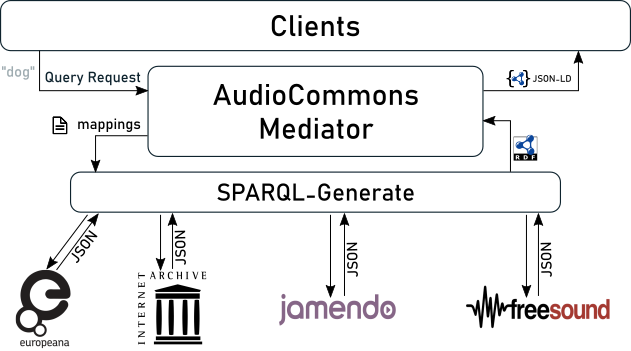
\includegraphics[width=0.9\textwidth]{audiocommons_schema.png}
\caption{Schema of the AudioCommons Mediator working logic.}
\label{fig:ac_schema}
\end{figure}

Fig.~\ref{fig:ac_schema}, instead, takes a different direction: the \textit{dog} request is given to a service called \texttt{SPARQL-Generate} \cite{lefranccois2017sparql, lefranccois2016flexible} together with a set of \textit{mappings}. Each mapping is specific for a content provider, and carries the needed information to correctly contact the provider and to interpret and parse the expected output.

In our setup, available on Github\footnote{\faGithub~\url{https://github.com/AudioCommons/semanticMediator}}, the mapping has to translate the outputs from Europeana, the Internet Archive, Freesound and Jamendo, which are given in JSON format, into a shared semantic RDF graph. This is the \textit{generate} phase. This procedure, of course, implies that
\begin{enumerate}
\item The mapping contains all the needed information to correctly contact the content provider;
\item The \texttt{SPARQL-Generate} request is made having prior knowledge of the AC Ontology, essential to correctly format the RDF graph;
\item The \texttt{SPARQL-Generate} request is made having prior knowledge of the schema used by the media provider to build its JSON output;
\item Adding a new provider to the mediator means simply adding a new mapping, resulting in a setup that is extremely flexible and extensible.
\end{enumerate}

The RDF graph eventually obtained from the \texttt{SPARQL-Generate} after querying the four providers is the actual result of the process. It can be stored in a knowledge base, like Blazegraph or Virtuoso, for further usage. Alternatively, it can be simply returned back to the original client.

A further development of this unification procedure is connected to particular queries that need a long time to be performed, like the one suggested by Xamb\'o et al.~\cite{xambo2018jam}. In the next Section \ref{sec:siot_sepa} we will introduce an additional tool that is one of the core instruments of this Thesis, i.e. the SEPA. By using the SEPA, as it will be shown, it will be possible to address the long-query problem with a fully semantic setup.

\section{SPARQL Event Processing Architecture}
\label{sec:siot_sepa}

This Section will introduce one of the core tools that allowed the realization of the work outlined in this Thesis, i.e., the SPARQL Event Processing Architecture (SEPA). As a complete discussion on the internal specific mechanism of SEPA is out of the scope of this report, we will make some references to the published research \cite{roffia2018dynamic}, and present a higher level explanation.

Some light examples will also be shown, although the real test bench application can be found in Section \ref{sec:swot_ontology}, where the SEPA will represent the core engine supporting of our vision of Semantic Web of Things agents.

\subsection{Origins}

The SPARQL Event Processing Architecture is the last step of a long path made of ideas and projects in which ARCES research center has been involved since approximately 2010. At the time the idea was expressed in the Smart-M3 platform \cite{honkola2010smart}, which had the intent of implementing a middleware architecture to support information sharing among devices and software. The challenge of data interoperability was addressed through a semantic approach: applications would agree on an ontological description of data, and use a shared semantic endpoint to store their information.

An additional requirement, in this middleware setup, is dynamicity. This is due to the fact that dealing with devices and software is not a static task, but rather is something that is subject to continuous change. As a matter of fact, while the Smart-M3 architecture started to be applied also to IoT, this aspect became even more relevant. 

Addressing dynamic data exchange, in this context, created over the time the concept of Publish-Subscribe: according to \cite{eugster2003many}, a few types of Publish-Subscribe can be outlined. Well known and frequently used protocols, like AMQP and MQTT belong to the \textit{topic based} methodology for which, in a broad view, the \textit{topic} is a tag that identifies a communication channel. A \textit{content based} approach, instead, will simultaneously define a tag for the channel and request some further conditions on the data exchanged (e.g., if the channel is tagged \texttt{Temperature}, we call for \texttt{Temperature>25} degrees). The \textit{type based}, eventually, tag the channel with the format of the data that is passing.

The Smart-M3 architecture, in such panorama, is positioned as we said including part of each of the three aforementioned ideas plus a semantic approach. The middleware was implemented in various flavors, keeping nevertheless the reference to its function as a \textit{Semantic Information Broker}. It is possible to cite some of the implementations, namely RedSib \cite{morandi2012redsib}, OSGi SIB \cite{manzaroli2010smart}, CuteSIB \cite{galov2015design}, PySIB \cite{viola2016modular}: they were largely exploited and evaluated \cite{Viola2016PerformanceES,viola2016m3}, implement approximately the same paradigm and the same (non standard) protocols to perform semantic data insertion/deletion and subscription.

SEPA starts from that point on. With the appearance of the concepts of Web of Things and Linked Data, the semantic middleware needed to be updated in order to be compliant to web standards. In the next Section this complete refactoring is explained.

\subsection{Architecture}

SEPA's working logic is rather simple. It is a semantic middleware for interoperability that has to
\begin{enumerate}
\item Store and retrieve semantic data upon request;
\item Add and delete semantic data;
\item Control the evolution of data dynamically and notify changes;
\end{enumerate}
\begin{figure}[t!]
\centering
\includegraphics[width=\textwidth]{sepa_internal_architecture.png}
\caption{SEPA internal setup, from \cite{roffia2018dynamic}.}
\label{fig:sepa_schema}
\end{figure}
The clients, in such context, will require their data to be safely kept: to do so, SEPA relies on external tools to store semantic information, like Blazegraph\footnote{\faLink~\url{https://www.blazegraph.com/}}, Fuseki\footnote{\faLink~\url{https://jena.apache.org/documentation/fuseki2/}} or Virtuoso\footnote{\faLink~\url{https://virtuoso.openlinksw.com/}}. These are RDF stores, that can be queried and updated by the means of SPARQL 1.1 Query and Update Language.

The event monitoring service is added by our architecture on top of the semantic storage. To better understand how such subscription engine works, consider Fig.~\ref{fig:sepa_schema}. In the figure we outline the various possible behaviors that we can expect from a client (i.e., the line on top of the schema). The box at the bottom, instead, represents the SPARQL endpoint, or equivalently an RDF store instance. 

Queries, as it is shown, pass almost in a transparent way through SEPA, with the only constraint that query and update requests cannot be executed out of order. Updates, on the other hand, are conceptually bound to the subscription engine, as their side effect is to generate notifications. They are both executed through HTTP POST.

Once an update is received, the actual triples to be added, and the ones to be removed, are matched to the list of subscriptions that are active. If the subscription SPARQL pattern corresponds to some of the triples in either way, then the notification is triggered, through Websocket. For a complete and precise description of every internal mechanism, please refer to \cite{roffia2018dynamic}.

Let us make a simple SEPA usage example, by calling back the \textit{actor genealogy} introduced in Section~\ref{sec:semantic_web}. Should we implement the algorithm proposed (available in Github\footnote{\faGithub~\url{https://github.com/fr4ncidir/HollywoodGenealogy}}), we could have a query approach like the following:
\begin{lstlisting}[language=bash]
$ python3 hollywoodgenealogy.py "Jack Nicholson" "Julia Roberts"
(0) :Jack_Nicholson starred with :George_Clooney in 
:Batman_(1989_film_series)
(1) :George_Clooney starred with :Julia_Roberts in :Ocean's_Eleven
\end{lstlisting}

Indeed, to stay up to date with this information, it is necessary to repeat the search, at least each time a new film starring either Jack Nicholson or Julia Roberts is released. SEPA subscription engine would avoid this query polling procedure: by making the subscriptions in Listings~\ref{listing:direct_query} and \ref{listing:indirect_query}, we can be notified if a film in which both the actors have a role is updated to DBpedia. Furthermore, as it can be seen, the SPARQL that identifies the subscription is the same that is posted for the simple query.
%\begin{multicols}{2}
\begin{lstlisting}[label={listing:direct_query}, caption={Subscription to new direct connections}]
SELECT ?film1 WHERE {
 ?film1 dbpo:starring dbpedia:Julia_Roberts,dbpedia:Jack_Nicholson.
}
\end{lstlisting}
%\columnbreak
\begin{minipage}{\linewidth}
\begin{lstlisting}[label={listing:indirect_query}, caption={Subscription to new one-step connections}]
SELECT ?film1 ?actor_1 ?film2 ?actor_1 WHERE {
  ?film1 dbpo:starring ?actor_1, dbpedia:Julia_Roberts.
  ?film2 dbpo:starring ?actor_1, dbpedia:Jack_Nicholson.
}
\end{lstlisting}
%\end{multicols}
\end{minipage}

A slightly more complex example was already mentioned in the previous Section while discussing the European project AudioCommons. The AC Mediator, in this case, was designed to dispatch uniformed versions of query results coming from various services. By introducing their research Xamb\'o et al.~\cite{xambo2018jam} suggested a further expansion of the AC Mediator including in the queries some characters that may require audio analysis and elaboration. This activity, clearly, can be time-consuming and may cause scalability problems.

A SEPA powered solution to this challenge can be implemented as follows. We already said that query results are transformed into RDF graphs and then inserted into an RDF knowledge base. Let us consider a SEPA engine, in this case, with an underlying Blazegraph triple store. With reference to Fig.~\ref{fig:ac_schema}, we can modify the schema to include \textit{long queries} as it is shown in Fig.~\ref{fig:ac_schema_long}. Clients, here, make the request to the AC Mediator, that in this case is aware of what are the services that need the SEPA approach. If the incoming query request is one of them, the Mediator will (i) generate an URI to identify within the RDF store a subgraph in which results will be available in the end; (ii) use such URI to immediately reply to the client. With this information, the client is able to subscribe to the results of the query, and to be notified as soon as they are available (see Listing~\ref{listing:ac_long_subscription}) without blocking. 
\begin{figure}
\centering
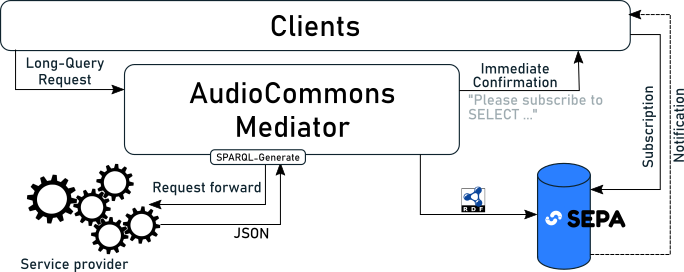
\includegraphics[width=\textwidth]{audiocommons_schema_sepa.png}
\caption{Schema of the AC Mediator working logic for long query services.}
\label{fig:ac_schema_long}
\end{figure}
\begin{minipage}{\linewidth}
\begin{lstlisting}[label=listing:ac_long_subscription,caption={Subscription example for the SEPA-enhanced AC Mediator.}]
SELECT * 
FROM <http://this_is_the_generated_uri>
WHERE {?a ?b ?c}
\end{lstlisting}
\end{minipage}

\subsection{Future}
As it was detailed, SEPA introduces a relevant dynamism to the semantic information. The IoT, in particular, will be the target of this in the prosecution of this Thesis, as by monitoring events we can follow the context evolution, and through semantics we can overcome the vertical silos fragmentation at information level.

However, SEPA presents various research opportunities for the future.

First of all, there is the need to study and enhance SEPA’s performances. SEPA, in fact, suffers of quick degradation of performances as the
number and complexity of subscriptions grows. Not to mention that the number of triples contained in the knowledge base has also a considerable impact on the subscription triggering engine. 

Secondly, following a technological trend of cloud distribution of services, a possible future direction is to work on a distributed SEPA, addressing a set of coherence and reliability issues that, to the best of the author's knowledge, have not yet been studied over linked data endpoints.

Eventually, RDF knowledge bases can be exploited with reasoning techniques. Their effect, in particular, is the modification of the knowledge base according to some rules. The SEPA architecture has not yet been tested with
reasoning, and therefore it could be interesting to see how SEPA and rule engines behave when used together in an application.
\clearpage

\chapter{Semantic Internet of Things}
\label{ch:iot}
\headletter{W}
ithin this Chapter a few facets of the Internet of Things will be discussed, highlighting in particular its integration with and within semantic technologies. Over the Sections some actual implemented ideas will explain which are the benefits of adding the semantic layer, both with a SEPA dynamic background, and without.

In addition to this, in Section~\ref{sec:iomust} we will completely present the first major contribution of this Thesis, i.e., the Internet of Musical Things ontology. Its main goal is to open the way to collaborative musical production, with connected musical devices. Although it may appear that we address a limited subset of the whole IoT, Section~\ref{sec:iomust} will give proof that the methodology is on the contrary general and open for further enhancements.


%In particular, some references will be made on the contents of Chapter~\ref{ch:background}. The references will be compared with the works available in literature in Section~\ref{sec:31_rw}, and in two research projects: Arrowhead and Habitat (Sections~\ref{sec:arrowhead}, \ref{sec:habitat}). During their life-cycle these two projects were involved in a process that is still going on at various levels, from academy to hobbyists and makers, to enhance the panorama of IoT with new opportunities, both for technology and for users. 
%
%In addition to this in Section~\ref{sec:iomust} a new paradigm of IoT will be explored: the IoT for music, aiming to  A full desciption will be provided, resulting in one of the major contributions of this Thesis.

\section{Semantic Interoperability}
\label{sec:21_rw}

Chapter~\ref{ch:background} gave a broad view of the IoT panorama. The addition of semantics, as we said, could represent a technique to overcome vertical fragmentation. As a matter of fact, interoperability was one of the leading ideas since the first appearances of the Semantic Web concept \cite{berners2001semantic}.

But what does \textit{interoperability} actually means? As we said in Section~\ref{sec:iot}, from a technical point of view the term interoperability implies that there should be, among the considered systems, the same ISO-OSI stack. Consequently, interoperability should allow systems to be aware of the existence of other systems regardless of how they internally work. Furthermore, a successful exchange of requests should also be possible, including failure robustness.

Discovery mechanisms, for this reason, represent the bigger difference among interoperable and non interoperable systems: they allow agent-awareness and, if implemented at higher level, also successful communication feedback. Literature is rich, in this sense, and over the time provided a plethora of examples, middlewares and projects, some of which have been already cited. They, however, often operate in a closed environment, and mostly assume that parallel projects, whenever interested in a collaboration, should be reprogrammed to be compliant with their view.

The Semantic Web overcomes this required parallelism at information level as shown in Fig.~\ref{fig:honeycomb}. As it can be seen, the Semantic Internet of Things keeps its specific implementations, assumptions and realizations (the ``\texttt{app}'' boxes). However, while the incompatibilities in previous IoT were either not treated, or case by case solved with complex elaboration, we here transform it in semantic subgraphs that can coexist.
\begin{figure}
\centering
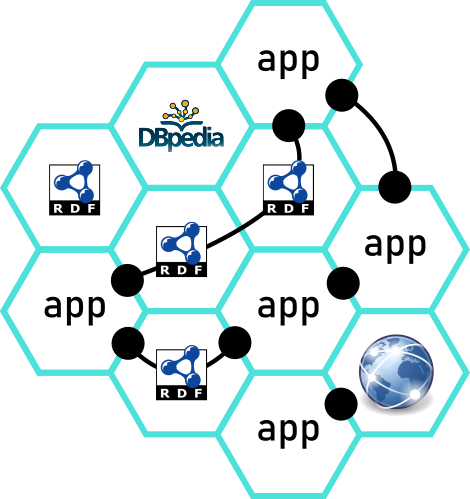
\includegraphics[scale=0.55]{honeycomb.png} 
\caption{Conceptual vision of the Semantic IoT. Local applications can directly communicate with each others, or with the Internet. Alternatively, they can share data through RDF formatting according to one or more ontologies.}
\label{fig:honeycomb}
\end{figure}

Consequently, interoperability is in this Section granted among collaborating systems relying on a continuous process of ontological inclusion. Such process was also targeted by previous research (e.g., \cite{halpin2010owl, calvanese2015ontology}). The Internet of Musical Things Ontology (see next Section) in this context provides a methodology to create such inclusion. The choice of a musical background, furthermore, is not limiting the suggested view: the core of the ontology, in other environments, is the common IoT universe (i.e. the \texttt{iot} namespace). The goal of Section~\ref{sec:iomust} is to setup an ontology by joining together other preexisting ontologies and taxonomies. Besides the innovative result materializing the IoMust in the Semantic Web panorama, one of the related outcomes is the interoperability achieved with IoMusT and any application made on top of the provided ontology components.

In Chapter~\ref{ch:semantic_wot}, in a different way, we will provide a broader view (but still semantically compatible with the present one), which includes also the web resources, unifying the Web and the IoT in the WoT over a semantic platform exploiting also SEPA.

\section{Internet of Musical Things}
\label{sec:iomust}
This Section takes inspiration from a recently submitted research paper: \faCopyright~~Turchet, L., Antoniazzi, F., Viola, F., Giunchiglia, F., \& Fazekas, G. (2019). The Internet of Musical Things Ontology. Submitted to~\textit{Journal of Web Semantics.}.

The Internet of Musical Things (IoMusT) is an emerging research area consisting of the extension of the Internet of Things paradigm to the musical domain. This field is positioned at the confluence of music technology, the Internet of Things, human-computer interaction, and artificial intelligence, and relates to the networks of computing devices embedded in physical objects (Musical Things) dedicated to the production and/or reception of musical content. Considering the computer science perspective, Turchet and colleagues \cite{turchet2018IoMusT} defined a Musical Thing as 
\begin{quote}
\textit{a computing device capable of sensing, acquiring, processing, or actuating, and exchanging data serving a musical purpose}
\end{quote} 
and defined the IoMusT as 
\begin{quote}
\textit{the ensemble of interfaces, protocols and representations of music-related information that enable services and applications serving a musical purpose based on interactions between humans and Musical Things or between Musical Things themselves, in physical and/or digital realms. Music-related information refers to data sensed and processed by a Musical Thing, and/or exchanged with a human or with another Musical Thing}
\end{quote}
  
Various kinds of Musical Things can be envisioned, which may be categorized according to the musical purpose they serve (e.g., to control, generate, or track responses to musical content). Examples of existing Musical Things are the ``smart musical instruments'', a new family of musical instruments encompassing sensors, actuators, wireless connectivity, and on-board processing \cite{turchet2019SMI}. These musical devices are able to directly exchange musically-relevant information with one another as well as communicate with a diverse network of external devices, such as smartphones, wearables, virtual reality headsets, or stage equipment. Instances of smart musical instruments include the Smart Caj\'{o}n reported in \cite{turchet_smartcajon_hit_2018} and the Sensus Smart Guitar developed by MIND Music Labs~\cite{turchet2017examples}. Another example of Musical Things are ``musical haptic wearables'' \cite{turchet_codesignMHW_2019}, a novel class of wearable devices embedding haptic stimulation, tracking of gestures and physiological parameters and wireless connectivity features. On the one hand, such devices were conceived to enhance communication between performers as well as between performers and audience members by leveraging the sense of touch in both co-located and remote settings. On the other hand, they were devised to enrich musical experiences of audiences of music performances by integrating haptic stimulations, as well as provide new capabilities for creative participation thanks to embedded sensor interfaces.  

Musical Things are connected by an infrastructure that enables multidirectional communication, both locally and remotely, between different stakeholders such as composers, performers, audience members, audio producers, live sound engineers, as well as music students and music teachers. The ecosystems that will form around Internet of Musical Things technologies are envisioned to support novel forms of interactions between such stakeholders by means of novel musical applications and services. This has the potential to revolutionize the way music is composed, performed, experienced, learned, and recorded. 

To accomplish the IoMusT vision, the Musical Things within an ecosystem need to dialog through a common language. A central unsolved issue within the IoMusT paradigm is how facilitating interoperability among heterogeneous Musical Things, which may serve radically different purposes (e.g., real-time analysis of musical content, generation and delivery of haptic, visual, or olfactory sensory layers additional to the musical content, delivery of content-recommendation services for music students). To date, interoperability across musical devices has mostly relied on protocols for the exchange of musical messages such as Musical Instrument Digital Interface (MIDI) or Open Sound Control (OSC) \cite{Wright2003OSC} and tools based on it (e.g., libmapper \cite{malloch2015distributed}). 

However, the existing musical protocols are not adequate to support interoperability across the wide heterogeneity of Musical Things, as they are typically not flexible, lack high resolution, not equipped with inference mechanisms, and do not support the integration with the Web. Semantic technologies, such as semantic web \cite{berners2001semantic} and knowledge representation \cite{sowa2000knowledge}, possess these features. For this reason, they have been recently envisioned as a solution to enable interoperability across heterogeneous Musical Things~\cite{turchet2018IoMusT}. Existing ontologies devised for the musical domain to date, such as the Music Ontology~\ontoref{music}, the Studio Ontology~\ontoref{studio} or the Audio Features Ontology~\ontoref{afo}, are insufficient to represent the wide knowledge base that the variety of the possible Musical Things entail. An ontology specific to the IoMusT scenario is currently missing. As a consequence, the use of semantic technologies in Internet of Musical Things contexts is limited to scenarios involving homogeneous Musical Things serving similar musical purposes or ad-hoc interactions designed for a specific, fixed scenario. 

The first effort towards the application of semantic technologies to the IoMusT context is reported in \cite{turchet2018sepa}. The authors proposed a semantically-enriched Internet of Musical Things architecture relying on a semantic audio server and edge computing techniques. Specifically, a SPARQL Event Processing Architecture \cite{roffia2018dynamic} was employed as an interoperability enabler allowing multiple Musical Things to cooperate, relying on a music-related ontology. A limitation of the developed architecture was the involvement of an ontology restricted to the representation of simple musical features, which prevented Musical Things dedicated to purposes other than music generation to join the ecosystem formed around the architecture.

Semantic technologies based on an ontology for the IoMusT can assist in managing, querying, and combining information characterizing an IoMusT ecosystem, including data about the music produced, the involved stakeholders, the utilized Musical Things and their application and services. This has the potential to spur the exploration of novel artistic avenues, such as performance and composition, for instance based on emergent properties of an IoMusT ecosystem \cite{ulieru2011emergent}. 

In this Section the ``Internet of Musical Things Ontology''~\ontoref{iomust} is exposed. The full design and evaluation process of the IoMusT Ontology is hereby given from the beginning to the current version, i.e., 1.0.0. The description of the IoMusT Ontology follows the MIRO (minimum information for the reporting of an ontology) guidelines~\cite{matentzoglu2018miro}. For reference, the paper reports the MIRO designations (e.g., E.9 for Ontology relationships), where the specific information item is provided. The ontology name (A.1) and its need (B.1) have been already introduced. The ontology is available on the web (see \ontoref{iomust}) (A.4) with license GPL3 (A.3).

\subsection{Methodology, audience, and scope}
This section describes the methodology adopted for the design and development of the IoMusT Ontology, as well as the audience of the ontology and its scope.

\subsubsection{\textsf{Methodology for ontology development}}
The ontology is developed and maintained by the authors and other members of the emerging IoMusT research community, which is currently composed by leading research institutes in sound music computing and Internet of Things (A.2 and C.2).

The design and development of the IoMusT Ontology was mostly inspired by the \textit{Methontology} methodological framework~\cite{fernandez1997methontology} (A.6). Such a framework is composed by six phases: i) the specification, i.e., the identification of the audience, scope, scenarios of use, and requirements; ii) the conceptualization of an informal model; iii) the formalization of the ontology namespaces, classes and properties; and iv) the integration of existing ontologies in a description and its reproduction in an OWL2 file \cite{motik2009owl}; v) the implementation of the ontology with an appropriate serialization language; vi) the maintenance of the ontology once implemented.

Moreover, the aforementioned framework identifies three tasks that are accomplished during the whole life of the ontology, which are orthogonal to the five phases: i) knowledge acquisition through research of related ontologies and models as well as gathering data from potential users), to inform multiple phases of the design process, mainly conceptualization and integration; ii) documentation of the process phases (internal) and the ontology specification (public); iii) the evaluation of the ontology before its release. 

Other works, like Uschold~\cite{uschold1996building} and more recently by De~Nicola et al.~\cite{de2016lightweight} suggest different methodologies for ontology engineering. These papers however include techniques that aim to formalize the setup from scratch of new ontologies. This is not the case in the current research, where the goal is to provide a new contribution based as much as possible on the integration of pre-existing contents.

\subsubsection{\textsf{Scope and audience}}
\label{ssec:audience_scope}
The role of the IoMusT Ontology is to offer a common data model enabling interoperability among heterogeneous Musical Things, which allows both people and virtual agents to seamlessly generate, explore, access, or transform music-related content produced within an IoMusT ecosystem. Therefore, the scope of the ontology (C.1) is represented by all ecosystems forming around existing or future IoMusT technologies.

The target audience of the ontology (B.3) is represented by all actors and stakeholders that are involved in such ecosystems, including performers, audience members, composers, studio producers, live sound engineers, and choreographers. 

\subsection{Related ontologies and data models}
\label{ssec:iomust_rw}
Before defining an ontology specific to the IoMusT domain we conducted a review of existing ontologies. The IoMusT vision is intrinsically multisensory and highly interdisciplinary \cite{turchet2018IoMusT}. This section describes ontologies and data models (B.2) that are related to such a vision. They have been gathered through the research of literature and online resources (D.1 and D.2) and evaluated as part of the design process (D.3).

\subsubsection{\textsf{Ontologies for the audio domain}}
Several ontologies have been proposed in recent years for the audio and music domains, in recognition of the complexity and broad ranging applications of such ontologies, and the fact that much of the information exchanged on the Web today is multimedia, of which music is a very substantial component, rather than text. The scope of such ontologies are wide ranging, starting from very focused areas of music production such as audio effects \cite{wilmering2013the}, to larger binding ontologies that target the description and retrieval of audio resources on the web in general \cite{ceriani2018audio}.

The Music Ontology (MO) \ontoref{music} \cite{raimond2007music, raimond2010spec} is a general purpose high-level ontology for the music domain that models the music value-chain from production to consumption. Therefore its focus is on editorial metadata, e.g. artist name and title associated with audio recordings, as well as the representation of major steps in the production of recorded music, from composition, through performance and recording, to release.

The Music Ontology does not deal with the nuances of technical workflows in music production. This is the area covered by the Studio Ontology \ontoref{studio} (SO) \cite{fazekas2011studio}. 

The Audio Features Ontology \ontoref{afo} (AFO) addresses another audio domain that requires detailed conceptualisations. Audio Features are descriptors that represent specific characteristics of sound signals. These may relate to measurable properties of the signal, such as bandwidth or spectral centroid, perceptual qualities like pitch and loudness, and musical characteristics such as notes, musical key and chords.

The Musical Instruments Ontology \cite{kolozali2011knowledge} is highly relevant to the domain of IoMusT. It provides an ontological model for encoding well known instrument classification systems, e.g. for grouping instruments into categories such as \textit{Idiophones} or \textit{Aerophones}, based on their sound production or excitation mechanism.

The Audio Commons Ontology (ACO) \ontoref{aco} \cite{ceriani2018audio} is an example of a higher level domain ontology that binds several audio related ontologies together. It was designed to facilitate the integration of audio content repositories on the Web as well as content consumption by software agents. 

\subsubsection{\textsf{Ontologies for sensors, actuators and connectivity}}
Among the ontologies designed for the IoT, two of the most diffuse are SSN (Semantic Sensor Network) and SOSA (Sensor, Observation, Sample, and Actuator) \ontoref{ssn, sosa}. Both SSN and SOSA adopt a complex approach to description of hardware, observation of physical entities and actuation. SSN~\cite{compton2011ssn} covers the majority of the SensorML standard\footnote{\faLink~\url{https://www.opengeospatial.org/standards/sensorml}} and has been designed to describe sensors and observations, as well as the deployment in which sensors are employed. SOSA~\cite{janowicz2018sosa} adopts a lightweight approach to describe sensors, actuators and the acts of observation and actuation. SOSA acts as a replacement of the Sensor-Stimulus-Observation (SSO) design pattern provided by SSN, that provides greater expressivity~\cite{haller2018sosa}.

At a higher level of abstraction, things in IoT can be represented according to the Web Thing model\footnote{\faLink~\url{https://www.w3.org/Submission/wot-model/}} proposed by the W3C. In this sense, devices are provided with the so-called thing description, a detailed profile reporting properties, events and actions exposed through its interface. A first attempt to semantically represent this model has been provided by Charpenay et al. in~\cite{charpenay2016introducing}, later on envisioned by Serena et al. in~\cite{serena2018discovery} for a discovery framework. The Web of Things ontology discussed by Charpenay et al. and Serena et al. has been employed by Viola et al.~\cite{viola2018playsound} to build a semantic Web of Things enviroment for recommendations in the audio domain. Eventually, Antoniazzi et al.~\mbox{\cite{antoniazzi2019building}} provided a semantic version of the Web of Things.

\subsection{Specification}
\label{ssec:specification}
The acquired knowledge was then analzed to identify a set of requirements that the ontology should satisfy \cite{siegemund2011towards}. The literature review led to a total of 15 scenarios (5 scenarios from \cite{turchet2018IoMusT}, 5 from \cite{turchet2019SMI}, and 5 defined by the authors or derived from recent experiments with users described in the literature). For each scenario we derived a set of requirements, and then applied a thematic analysis \cite{BraCla06} to reduced them. The resulting requirements are represented below as a list of example questions that the ontology should be able to support answering \cite{gruninger1995methodology}, and a list of formal requirements.


\subsubsection{\textsf{Competency questions}}
The following sample questions are meant to be asked with respect to an IoMusT ecosystem:
\begin{multicols}{2}
\begin{enumerate}
\item Which type of Musical Things are used by the local and remote performers during the live concert?
\item How many Musical Things used by the audience provide haptic feedback?
\item What smart instruments are controlling the smartphones used by the audience?
\item What is the mood of the music at a given time during the live performance?
\item How many audience members are actively participating to the music creation process thanks to their Musical Things?
\item Which kind of stage equipment is used at a given time during the concert?
\item Which gestural and biometric parameters are tracked from the audience during the live performance?
\item How many and which kind of networks are used during a performance?
\item Which pedagogical applications are available for a smart violin?
\item With which music content repository a smart ukulele can interact?
\item Which services are available for a smart guitar and what are their purposes?
\item What type of sensors and actuators compose a smart musical instrument or a musical haptic wearable?
\end{enumerate}
\end{multicols}

\subsubsection{\textsf{Formal requirements}}
The IoMusT Ontology should be able to:
\begin{multicols}{2}
\begin{enumerate}

\item represent the concept of Musical Things, including: 
	\begin{enumerate}[wide, labelindent=0pt]
	\item its type (e.g., musical instrument, wearable device, stage equipment);
	\item its characteristics including the number and type of inputs (e.g., sensors tracking movements or biometric parameters) and outputs (e.g., auditory, visual, haptic, olfactory);
	\item the type of person for which it is conceived (e.g., performer, audience member, live sound engineer, producer); 
	\item its function (e.g., a smart instrument used to produce musical content, a musical haptic wearable aiming at enriching the listeners' musical experience, an interface used by audience members for participatory purposes, a device used to infer the mood of audience members based on sensed quantities);
	\item its geographical position;
	\item the type of data that it generates (e.g., audio signal, text message);
	\end{enumerate}
	
\item represent the concept of connectivity, including: 
	\begin{enumerate}[wide, labelindent=0pt]
	\item the type of network involved (e.g., local network, remote network, Wi-Fi-based, millimeter waves-based);
	\item the attributes of the network (e.g., bandwidth, speed, synchronization mechanisms);
	\item the time taken by the network to deliver/receive a message to/from a certain Musical Thing;
	\end{enumerate}

\item represent the concept of application and service, including:
	\begin{enumerate}[wide, labelindent=0pt]
	\item its purpose (e.g., for music learning, performance, composition, studio production)
	\item its level of interactivity (e.g., interactive, non-interactive)
	\item its type (e.g., social network, online music content repository)
	\item its user (e.g., composer, performer, studio producer, educationalist, student, audience member)
	\end{enumerate}

\item describe attributes of the music (produced live) at a given time, including:
	\begin{enumerate}[wide, labelindent=0pt]
	\item low-level features (e.g., the density of notes);	
	\item high-level features (e.g., the mood)
	\end{enumerate}	
	
\item describe attributes of the ecosystems, including:
	\begin{enumerate}[wide, labelindent=0pt]
	\item the number and type of Musical Things present in the network at a given time and a given space;
	\item which Musical Things are interacting;
	\item the number and type of applications and services available within the ecosystem; 
	\item the number and type of networks used at a given time.
	\end{enumerate}	

\end{enumerate}
\end{multicols}

\subsection{Ontology description}
\label{ssec:description}
The Internet of Musical Things ontology (the IoMusT Ontology) has been developed incrementally. As a matter of fact, the task of developing ontologies is in general complex, and needs an approach that involves continuous refinement and check of concepts and relationships. This can be done in several ways, and may be performed iteratively as long as the expected match of the ontology with the real subject is achieved. 

Not surprisingly, the first step is to split the domain of interest in smaller parts if possible. For each of those smaller parts, secondly, iterations are needed to ensure that all relevant concepts are included. Sometimes this is done by surveying a pool of experts and/or future users of the ontology, to get their feedback. Clearly, this check helps designers to avoid wrong naming on resources, as well as to detect and correct contradictory assertions.

Then, the smaller parts have to be joined together to form the ontology. Again, the expressiveness of the complete work has to be checked, and in this paper this is provided by requirement analysis and evaluation. The question to be answered, here, is: \textit{is my ontology capable to describe my context? If so, is the description made with the precision needed?} This process also may be performed iteratively.

IoMusT Ontology is not an exception. On the contrary, it is very important to notice that the formalization of a vocabulary for Internet of Musical Things needs this feedback process to ensure a coherent representation of music-related entities with general-purpose contents. 

A bottom-up process was deployed for our case. In particular, jumping from wider to narrower concepts, the first idea to be discussed is indeed the connection that stands between the global interpretation of Internet of Things and how to decline it into the Internet of Musical Things. See also Fig.~\ref{fig:fig1}. Clearly, the former is larger than the latter, which should represent a specialization and rely on it. The usage of the IoMusT Ontology, as a consequence, should allow a transparent view of any Musical Thing context as an IoT system. There would be no point in ignoring this core aspect, because the core idea of ontology engineering is to provide a shared and interoperable way to collaborate between different fields of knowledge. Any design choice opposed to this view would have as a direct result the creation of another vertical silos within the IoT chaos \cite{broring2017enabling}.

In order to replicate in the ontology this necessary duality, this work will suggest the adoption of two new namespaces:
\begin{enumerate}
    \item \texttt{iot}, that will be used to connect concepts that belong to the broader view of generic devices;
    \item \texttt{iomust}, which is an extension of \texttt{iot} defined as \texttt{iot:musical}. Within this namespace are organized the concepts of music-related IoT;
\end{enumerate}

For the sake of clarity the prefixes are kept in a contracted form. To see their expanded version, please see the \hyperref[sec:ontology_list]{List of Ontologies}.

\subsubsection{\texttt{iot} \textsf{namespace}}

The first concept to be defined is the \textit{Thing} as it is intended in the acronym IoT. Liu et al.~\cite{liu2016comparison} survey and comment the spectrum of definitions that have been suggested in literature over the time. Among the surveyed entries, the one proposed by the IEEE is coherent with our requirement of generality: the thing 
\begin{quote}
\textit{is any physical object relevant from a user or application perspective}
\end{quote} 
meaning that we consider things as items exploiting, or being exploited by, other items. Therefore, from now on, the class \texttt{iot:Thing} has to be considered according to this definition. Notice that also regular everyday life objects may be \texttt{iot:Thing}s, like chairs, pillows, a scarf, a painting and, indeed, a musical instrument.

Clearly, this is a generic class that needs to be further specialized in subclasses. Again, a lot of help can come from the listings in \cite{liu2016comparison}, as \texttt{iot:Thing} is definitely a huge container. For instance, things can be wearable objects: so, the class \texttt{iot:WearableThing} can be defined to represent this category. Similarly, devices can also be \textit{smart}, so we call for \texttt{iot:SmartThing} class: smart things, e.g., a smartphone, a smart TV, include special technological features or artifacts that provide them with relevant added value over the basic version of the same object. 

Eventually, things can be connected to a communication network: they are, in this case, instances of the class \texttt{iot:ConnectedThing}. Notice that the aforementioned Studio Ontology \ontoref{studio} contains a rich environment of properties and classes related to connectivity (e.g., the \textit{Connectivity} and the \textit{Device} sub-ontologies). %Fully including it in the IoMusT Ontology is a task that goes beyond the scope of this paper, but still it is a future project, as it may be a direct answer to some competency question & requirements.

It would neither be reasonable, nor useful, to list here a hundred of possible subclasses. For this reason, in the present paper only a few will be defined, as the discussion requires them. It is important to notice that there is complete freedom to include new classes whenever needed, as this is precisely the kind of incremental approach for ontology engineering which was above aforementioned.

\subsubsection{\textsf{Musical things in the \texttt{iomust} namespace}}

IoMusT Ontology, as already said, aims to develop the \texttt{iot} namespace in its musical flavour. To do so, the reference to a vocabulary connected to music is essential. Our reference in this work was introduced in Section~\ref{ssec:iomust_rw}: it is the Music Ontology~\ontoref{music}, which will be mentioned as the \texttt{music} namespace. An important contribution of this namespace in IoMusT Ontology is its supporting role in creating the archetype of Musical Thing, i.e. the class \texttt{iomust:MusicalThing}. In the present work, our definition for this class is the following: the Musical Thing is \textit{a thing used to produce or enjoy music, with reference to its context}. As a consequence, IoMusT Ontology will consider that a smart loudspeaker, a CD by David Bowie belong to that class, as well as a smart violin located in a concert hall. The same smart violin, however, if stored for exposition in a museum, is no more an \texttt{iomust:MusicalThing} because it loses its musical production interest. 

The class \texttt{iomust:MusicalThing} is indeed less generic than its superclass \texttt{iot:Thing}, because it provides a light form of contextualization. Yet, however, we need more precise solutions to be even less abstract. All the items identified in the example above (the smart loudspeaker, the CD, the smart violin) would point to \texttt{iot:Thing} through the \texttt{rdf:type} predicate. Then, to include an explicit reference to music, and introduce the Internet of Musical Things namespace, the following rule applies:
\begin{rul}
\label{rule:musical_thing}
    If an \texttt{iot:Thing} instance is also connected through \texttt{rdf:type} to a class belonging to the Music Ontology, then it is also an instance of \texttt{iomust:MusicalThing}. 
\end{rul}
A typical application of Rule~\ref{rule:musical_thing} is the aforementioned smart violin:  consider Expression~\ref{listing:violin_1} as an example, where a simple triple representation is given of the implication expressed. Notice that Rule~\ref{rule:musical_thing} is not intended to be strictly reversible: during a concert, lights and smoke machines may be intended as Musical Things because of their essential contribution to the listening experience, and yet may not be included in one of the \texttt{music} namespace categories. 
\begin{multline}
\label{listing:violin_1}
\texttt{ns:SmartViolin a iot:Thing, music:Instrument} \\ \Rightarrow \texttt{ns:SmartViolin a iomust:MusicalThing}
\end{multline}

%\begin{lstlisting}[caption={Triple representation of Rule~\ref{rule:musical_thing}. Extended prefixes are available in Table~\ref{tab:prefixes}.}, label={listing:violin_1}, mathescape]
%ns:SmartViolin a iot:Thing, music:Instrument
%$\Rightarrow$
%ns:SmartViolin a iomust:MusicalThing
%\end{lstlisting}
The Generic Musical Thing definition is not enough to build the complete IoMusT. Here it follows a sequence of new classes to be introduced in the \texttt{iomust} environment, descending from the Musical Thing. Each of the classes here corresponds to a rule similar to Rule~\ref{rule:musical_thing} in the OWL.
\begin{description}[wide, labelindent=0pt]
\item[\texttt{iomust:SmartMusicalThing}] is a Musical Thing that is also an \texttt{iot:SmartThing};
\item[\texttt{iomust:SmartInstrument}] is a Musical Thing that is also a \texttt{music:Instrument};
\item[\texttt{iomust:WearableMusicalThing}] is a Musical Thing that is also an \texttt{iot:WearableThing};
\item[\texttt{iomust:StageEquipment}] is a collection of Musical Things serving as equipment. The definition of collection can be extracted from external ontologies designed \textit{ad hoc} for this, like \ontoref{collection}.
\end{description}

Table~\ref{tab:musical_thing_examples} contains some practical examples of usage for the \texttt{iot} and \texttt{iomust} namespace entities.

\begin{table*}[t]
    \centering \footnotesize
    \caption{Example of usage for \texttt{iot} and \texttt{iomust} namespaces. We here show how objects part of an Internet of (Musical) Things environment can be considered instances of the classes introduced in this research. Extended prefixes are available in the \hyperref[sec:ontology_list]{List of Ontologies}.}
    \label{tab:musical_thing_examples}
    \vspace{3mm}
    \begin{tabular}{r|c|c|c|c|c|c|c|c|c|}
     & \rotatebox{90}{\texttt{ns:Bob}} & \rotatebox{90}{\texttt{ns:Wardrobe}} & \rotatebox{90}{\texttt{ns:SmartCar}} & \rotatebox{90}{\texttt{ns:Violin}} & \rotatebox{90}{\texttt{ns:SmartViolin}} & \rotatebox{90}{\texttt{ns:TShirt}} & \rotatebox{90}{\texttt{ns:StageLight}} & \rotatebox{90}{\texttt{ns:VR\_HeadSet}} &
     \rotatebox{90}{\begin{tabular}{@{}c@{}}\texttt{ns:HeartBeatSensor} \\ for music experiment \end{tabular}} \\
     \hline
    \texttt{foaf:Person} & \faCheck  &  &  &  &  &  &  &  &\\ \hline
    \texttt{iot:Thing} &  &  \faCheck &  \faCheck & \faCheck  & \faCheck & \faCheck  & \faCheck  & \faCheck & \faCheck \\ \hline
    \texttt{iot:SmartThing} &  &  &  \faCheck &  &  \faCheck &  & \faCheck & \faCheck & \\ \hline
    \texttt{iot:ConnectedThing} &  &  &  &  &  \faCheck &  & \faCheck & \faCheck & \faCheck \\ \hline
    \texttt{iot:WearableThing} &  &  &  &  & & \faCheck &  &  \faCheck & \faCheck \\ \hline
    \texttt{music:Instrument} &  &   &  & \faCheck &  \faCheck &  &  &  & \\ \hline
    \texttt{iomust:MusicalThing} &  &   &  & \faCheck  &  \faCheck &  &  \faCheck &  & \faCheck \\ \hline
    \texttt{iomust:SmartMusicalThing} & &  &   &  &  \faCheck &  & \faCheck  &  & \\ \hline
    \texttt{iomust:SmartInstrument} &  &  &  &  &  \faCheck &  &  &  & \\ \hline
    \texttt{iomust:StageEquipment} item &  &  &  &  &  &  & \faCheck &  &  \\ \hline
    \texttt{iomust:WearableMusicalThing} &  &  &  &  &  &  &  &  & \faCheck\\ \hline
    \end{tabular}
\end{table*}

\subsubsection{\textsf{\texttt{iot} \& \texttt{iomust} sensing, actuating and interacting}}
So far the discussion on the IoMusT Ontology was conducted as a set of broad definitions for the baseline concepts. Here, instead, space is given to how the integration of other ontologies enables our vision of  the IoMusT from a lower level standpoint.

First of all it is necessary to describe the smart devices more in detail, and include additional information related to the electronic devices embedded in the \texttt{iot:Thing} (e.g., micro-controllers, sensors, actuators). The \texttt{iot:SmartThing} was previously introduced to this effect, though without any other specificity. Consequently, to provide greater precision on the actual available sensing and actuating units, other information is needed. Taking into  consideration Table~\ref{tab:musical_thing_examples} as an example, we have to provide a way to semantically distinguish between two instances of \texttt{iot:SmartThing}, like the smart violin, and the virtual reality headset, based on their setup. To achieve such goal, this work suggests the inclusion of an ontology already existing and well known in the panorama, namely, SOSA \ontoref{sosa}. The choice of SOSA has three main advantages that greatly benefit IoMusT Ontology: (i) SOSA is \textit{de facto} a light version of SSN, and therefore the IoMusT Ontology can be furtherly extended towards SSN integration very easily; (ii) SOSA is very simple, which is always a relevant factor when studying, building and integrating ontologies; (iii) SSN and SOSA, eventually, are a relatively recent W3C recommendation (the last draft dates back to 2017), which means that they are globally accepted as a reference.

The realization of this ontological alignment is made by including as a plug-in the concept of \texttt{sosa:Platform} in the IoMusT Ontology subgraph for the \texttt{iot:Thing} and its aforementioned subclasses. According to SOSA documentation, the \texttt{sosa:Platform} is an \textit{entity that hosts other entities, particularly Sensors, Actuators, Samplers, and other Platforms}, that is precisely the facet missing until now in the \texttt{iot} namespace. In 
%Listing~\ref{listing:sosa_example} 
Fig.~\ref{graph:sosa_example}
a few examples are provided to show how the connection can be made. As it can be seen, the smart guitar instance \texttt{ns:SmartGuitar} has also as \texttt{rdf:type} the \texttt{sosa:Platform} class. This additional type allows us to include references to the sensors and actuators on board, as well as the entity they measure. Further details on sensing and measurement description, extensively discussed in previous researches like \cite{rijgersberg2013ontology, narock2009using} and surveyed in \cite{wang2015survey}, are out of the scope of this paper. For the future, anyway, the possibility to integrate new ontologies still exists: for the ones exploiting SOSA and SSN, such process should be trivial.

\begin{figure*}[h!]
\begin{center}
\begin{tikzpicture}[->,>=stealth']

\node[state,draw=mauve!90,fill=mauve,text=white,align=center] (SMARTGUITAR) {
\begin{tabular}{l}
  \parbox{2.6cm}{\texttt{ns:SmartGuitar}}
   \end{tabular}
};
  
 % State: ACK with different content
 \node[state,  yshift=2.4cm, right of=SMARTGUITAR, node distance=3cm, anchor=center, draw=yellow!90,fill=yellow!90,align=center] (SGTYPES) {%
    \begin{tabular}{l} 
        \parbox{4.8cm}{\texttt{iot:Thing, sosa:Platform, iot:SmartThing, iomust:MusicalThing, music:Instrument, iomust:SmartInstrument, iomust:SmartMusicalThing;}}
    \end{tabular}
};
  
   % State: ACK with different content
\node[state, yshift=0cm, right of=SMARTGUITAR, node distance=6.5cm, anchor=center, draw=mauve!90,fill=mauve!90,align=center,text=white] (IMUSENSOR) {%
    \begin{tabular}{l}
        \parbox{2.2cm}{\texttt{ns:IMUSensor}}
    \end{tabular}
};
  
\node[state, yshift=-1.5cm, right of=SMARTGUITAR, node distance=5cm, anchor=center, draw=mauve!90,fill=mauve!90,align=center,text=white] (CONTACTMIC) {%
    \begin{tabular}{l} 
        \parbox{3.8cm}{\texttt{ns:ContactMicrophone}}
    \end{tabular}
};
  
\node[state, yshift=-3cm, right of=SMARTGUITAR, node distance=1cm, anchor=center, draw=mauve!90,fill=mauve!90,align=center,text=white] (LOUDSPEAKER) {%
    \begin{tabular}{l} 
        \parbox{2.6cm}{\texttt{ns:Loudspeaker}}
    \end{tabular}
};
  
\node[state, yshift=0cm, right of=IMUSENSOR, node distance=4cm, anchor=center, draw=yellow!90,fill=yellow!90,align=center] (SENSORS) {%
    \begin{tabular}{l}
        \parbox{2cm}{\texttt{sosa:Sensor}}
    \end{tabular}
};
  
\node[state, yshift=0cm, right of=LOUDSPEAKER, node distance=5cm, anchor=center, draw=yellow!90,fill=yellow!90,align=center] (ACTUATORS) {%
    \begin{tabular}{l}
        \parbox{2.4cm}{\texttt{sosa:Actuator}}
    \end{tabular}
};
  
\node[state, yshift=0cm, right of=SGTYPES, node distance=5.5cm, anchor=center, draw=mauve!90,fill=mauve!90,align=center,text=white] (IMUHOSTS) {%
    \begin{tabular}{l} 
        \parbox{3cm}{\texttt{ns:Acceleration, ns:Rotation, ns:Orientation}}
    \end{tabular}
};
  
\node[state, yshift=-1.3cm,  right of=IMUHOSTS, node distance=3.5cm, anchor=center, draw=yellow!90,fill=yellow!90,align=center] (OBSERVABLEPROPERTY) {%
    \begin{tabular}{l} 
        \parbox{4.4cm}{\texttt{sosa:ObservableProperty}}
    \end{tabular}
};
  
\node[state, yshift=0cm, right of=CONTACTMIC, node distance=6.7cm, anchor=center, draw=mauve!90,fill=mauve!90,align=center,text=white] (VIBRATION) {%
    \begin{tabular}{l}
        \parbox{2.2cm}{\texttt{ns:Vibration}}
    \end{tabular}
};
  
\node[state, yshift=-1cm,  right of=LOUDSPEAKER, node distance=4cm, anchor=center, draw=mauve!90,fill=mauve!90,align=center,text=white] (SOUND)  {%
    \begin{tabular}{l} 
        \parbox{1.4cm}{\texttt{ns:Sound}}
    \end{tabular}
};
  
\node[state, yshift=0cm, right of=SOUND, node distance=5cm, anchor=center, draw=yellow!90,fill=yellow!90,align=center] (ACTUATABLEPROPERTY) {%
    \begin{tabular}{l}
        \parbox{4.4cm}{\texttt{sosa:ActuatableProperty}}
    \end{tabular}
};
 
\path (SMARTGUITAR)     edge[bend left=30,draw=blue]  node[anchor=north,above]{\textcolor{blue}{\texttt{a~~}}}   (SGTYPES)
(SMARTGUITAR)   edge[anchor=south,draw=blue] node[]{\textcolor{blue}{\texttt{sosa:hosts}}}                      (IMUSENSOR)  
(SMARTGUITAR)   edge[bend right=10,draw=blue] node[anchor=south, below]{\textcolor{blue}{\texttt{sosa:hosts}}}  (LOUDSPEAKER)  
(SMARTGUITAR)   edge[bend right=20,draw=blue] node[anchor=south, above]{\textcolor{blue}{\texttt{sosa:hosts}}}  (CONTACTMIC)
(IMUSENSOR)     edge[draw=blue] node[anchor=north]{\textcolor{blue}{\texttt{a}}}                                (SENSORS)
(LOUDSPEAKER)   edge[draw=blue] node[anchor=north]{\textcolor{blue}{\texttt{a}}}                                (ACTUATORS)
(CONTACTMIC)    edge[draw=blue] node[anchor=north]{\textcolor{blue}{\texttt{a}}}                                (SENSORS)
(IMUSENSOR)     edge[draw=blue] node[]{\textcolor{blue}{\texttt{sosa:observes}}}       (IMUHOSTS)
(IMUHOSTS)     	edge[bend left=30,draw=blue] node[anchor=north]{\textcolor{blue}{\texttt{a}}}                                (OBSERVABLEPROPERTY)
(CONTACTMIC)    edge[draw=blue] node[anchor=north]{\textcolor{blue}{\texttt{sosa:observes}}}                    (VIBRATION)
(VIBRATION)     edge[bend right=30, draw=blue] node[anchor=north]{\textcolor{blue}{\texttt{~~a}}}                                (OBSERVABLEPROPERTY)
(LOUDSPEAKER)   edge[bend right=10, draw=blue] node[below]{\textcolor{blue}{\texttt{sosa:actsOnProperty~~~~~~~~~~~~}}}         (SOUND)
(SOUND)     	edge[draw=blue] node[anchor=north, below]{\textcolor{blue}{\texttt{a}}}                                (ACTUATABLEPROPERTY);   

\end{tikzpicture}
\end{center}
\caption{SOSA integration with the IoMusT Ontology. Extended prefixes are available in the \hyperref[sec:ontology_list]{List of Ontologies}. The color scheme is the same used in Prot\'eg\'e \cite{protege}.\\Legend:~~\textbf{\textcolor{yellow!90}{Classes}~~\textcolor{mauve!90}{Individuals}~~\textcolor{blue}{Object Properties}}.}
\label{graph:sosa_example}
\end{figure*}

Sensing and actuating are in general part of a greater intent of interactive IoT system design. Data collection, then, provides the tools to create a feedback to control actuation and, eventually, to show smart behavior. Interaction is an unavoidable part of this process and, consequently, it should also be represented in the ontology alongside with sensors and actuators. Once such semantic prototype is given, it is possible to distinguish the active resources from the environmental passive ones and an interaction is finally possible. Besides, if the semantic view is shared among various systems horizontally, a strong and effective interoperability is automatically achieved.

The study of entities interacting within their environment is a well established field in literature, leveraging the concepts of \textit{agent} (e.g., \cite{jennings1999agent, leitao2016smart, kravari2015survey} and many others) and \textit{semantic agent} (see, for instance, \cite{hendler2001agents, lin2010modeling}). 

Within the IoMusT Ontology, the agent is referred to as any entity, human, object or virtual, that is capable of triggering any kind of dynamic evolution in an environment populated by instances of \texttt{iot:Thing} class. Both \texttt{iot} and \texttt{iomust} namespaces do not include directly such content, as their focus is the device, regardless the interaction aspect. For this reason, and for the discussion above, the IoMusT Ontology needs to rely on external ontologies to properly provide a definition of agent. Similarly to what has been suggested in the previous paragraphs with SOSA, we suggest here to exploit well-known ontologies, namely \ontoref{foaf} and \ontoref{prov}. 

The former, once connected to the IoMusT Ontology, defines the \texttt{foaf:Agent} as \textit{person, group, software or physical artifact}, and \textit{things that do stuff}. The idea of agent suggested in the previous paragraph is clearly derived from FOAF, although its real utility, in our research, is its capability of including the human being class \texttt{foaf:Person} and relationships in the semantic environment. Agents, intended as physical and virtual devices, are described through the latter, PROV-O, where the agent is \textit{something that bears some form of responsibility for an activity taking place, for the existence of an entity, or for another agent's activity} \cite{lebo2013prov}. This idea, in particular, includes also entities running software, which belong to \texttt{prov:SoftwareAgent}. Listing~\ref{listing:foaf_example} shows an example of using FOAF and PROV-O, and introduces in the \texttt{iot} namespace the ownership property \texttt{iot:owns}. 
\begin{lstlisting}[caption={FOAF \& PROV-O integration with the IoMusT Ontology. Extended prefixes are available in Table~\ref{tab:prefixes}.}, label={listing:foaf_example}]
ns:cristina     a   		foaf:Agent, foaf:Person, 
                    		prov:Agent, prov:Person;
                foaf:name 	'Cristina';
                iot:owns  	ns:SmartGuitar.
\end{lstlisting}
Ownership and actual usage do not necessarily coincide: it may happen, for instance, that people use a tool belonging to someone else. Besides, ownership does not imply any sort of activity with the device. A setup for activities, part of the IoMusT Ontology, is available in Fig.~\ref{graph:activities}.

\begin{figure*}[!ht]
\begin{center}
\begin{tikzpicture}[->,>=stealth']

\node[state,draw=mauve!90,fill=mauve!90,text=white,align=center] (BOB) {
\begin{tabular}{l}
  \parbox{1.1cm}{\texttt{ns:bob}}
   \end{tabular}
};
  
 % State: ACK with different content
 \node[state,  yshift=2cm, right of=BOB, node distance=4cm, anchor=center, draw=yellow!90,fill=yellow!90,align=center] (BOBTYPES) {%
    \begin{tabular}{l} 
        \parbox{3cm}{\texttt{foaf:Agent, foaf:Person, 
                music:Performer, prov:Agent, prov:Person;}}
    \end{tabular}
};

 % State: ACK with different content
 \node[state,  yshift=2cm, node distance=0cm, anchor=center, draw=green!90,fill=green!90,align=center] (BOBNAME) {%
    \begin{tabular}{l} 
        \parbox{0.9cm}{\texttt{'Bob'}}
    \end{tabular}
};
  
   % State: ACK with different content
\node[state, yshift=-2cm, anchor=center, draw=mauve!90,fill=mauve!90,align=center,text=white] (CRISTINA) {%
    \begin{tabular}{l}
        \parbox{2.1cm}{\texttt{ns:cristina}}
    \end{tabular}
};
  
\node[state, right of=BOB, node distance=6.9cm, anchor=center, draw=mauve!90,fill=mauve!90,align=center,text=white] (APPLICATION) {%
    \begin{tabular}{l} 
        \parbox{3.8cm}{\texttt{ns:IomustApplication}}
    \end{tabular}
};

 \node[state, right of=BOBTYPES, node distance=6cm, anchor=center, draw=yellow!90,fill=yellow!90,align=center] (APPLICATIONTYPES) {%
    \begin{tabular}{l} 
        \parbox{6cm}{\texttt{iot:Application, prov:Activity,
        iomust:MusicalThingApplication;}}
    \end{tabular}
};

\node[state, yshift=-1cm ,draw=mauve!90,right of=APPLICATION, node distance=5cm, fill=mauve!90,text=white,align=center] (SMARTGUITAR) {
\begin{tabular}{l}
  \parbox{2.6cm}{\texttt{ns:SmartGuitar}}
   \end{tabular}
};

\node[state,yshift=-1cm, 
%draw=purple!90,
right of=CRISTINA, node distance=6.5cm, 
%fill=purple!90,
%text=white,
align=center] (EVENT) {
\begin{tabular}{l}
  \parbox{1.2cm}{\texttt{\_:event}}
   \end{tabular}
};

 \node[state,  yshift=-1.5cm, right of=CRISTINA, node distance=12cm, anchor=center, draw=yellow!90,fill=yellow!90,align=center] (EVENTTYPES) {%
    \begin{tabular}{l} 
        \parbox{3.4cm}{\texttt{event:Event, prov:Entity, music:Performance;}}
    \end{tabular}
};

\node[state,yshift=-3cm, 
%draw=purple!90,
right of=CRISTINA, node distance=6.5cm,
%fill=purple!90,
%text=white,
align=center] (EVENTTIME) {
\begin{tabular}{l}
  \parbox{2cm}{\texttt{\_:eventtime}}
   \end{tabular}
};

\node[state,yshift=0cm, 
draw=yellow!90,fill=yellow!90,align=center,
right of=EVENTTIME, node distance=5cm,
align=center] (EVENTTIMETYPE) {
\begin{tabular}{l}
  \parbox{3.2cm}{\texttt{timeline:Interval}}
   \end{tabular}
};

 \node[state,  yshift=-3cm, right of=BOB, node distance=1cm, anchor=center, draw=green!90,fill=green!90,align=center] (STARTTIME) {%
    \begin{tabular}{l} 
        \parbox{4.1cm}{\texttt{'2019-06-18T12:00:00Z'}}
    \end{tabular}
};

 \node[state,  yshift=-5cm, node distance=0cm, anchor=center, draw=green!90,fill=green!90,align=center] (DURATION) {%
    \begin{tabular}{l} 
        \parbox{1cm}{\texttt{'PT1H'}}
    \end{tabular}
};
 
\path (BOB)     edge[draw=blue]  node[anchor=south,above]{\textcolor{blue}{\texttt{a}}}   (BOBTYPES)
(BOB)     edge[draw=green]  node[anchor=south,above]{\textcolor{green}{\texttt{foaf:name}}}   (BOBNAME)
(BOB)   edge[draw=blue] node[]{\textcolor{blue}{\texttt{foaf:knows}}}                      (CRISTINA)  
(BOB)   edge[draw=blue] node[anchor=south, above]{\textcolor{blue}{\texttt{iot:isInvolvedIn}}}  (APPLICATION)  
(APPLICATION)   edge[draw=blue] node[anchor=south, above]{\textcolor{blue}{\texttt{a}}}  (APPLICATIONTYPES)
(SMARTGUITAR)     edge[bend right=10, draw=blue] node[anchor=west]{\textcolor{blue}{\texttt{iot:isInvolvedIn}}} (APPLICATION)
(APPLICATION)   edge[draw=blue] node[text width=2cm]{\textcolor{blue}{\texttt{iot:produces,\\ prov:generated}}}                                (EVENT)
(EVENT)   edge[draw=blue] node[anchor=south west, text width=2cm]{\textcolor{blue}{\texttt{a}}}                                (EVENTTYPES)
(EVENT)   edge[draw=blue] node[text width=2cm]{\textcolor{blue}{\texttt{event:agent}}}                                (BOB)
(EVENT)   edge[bend right=10, draw=blue] node[text width=2cm]{\textcolor{blue}{\texttt{event:factor}}}                                (SMARTGUITAR)
(EVENT)   edge[draw=blue] node[anchor=south,text width=2cm]{\textcolor{blue}{\texttt{event:time}}}                                (EVENTTIME)
(EVENTTIME)   edge[draw=blue] node[anchor=south]{\textcolor{blue}{\texttt{a}}}                                (EVENTTIMETYPE)
(EVENTTIME)   edge[bend left=20,draw=green] node[anchor=south,text width=2cm]{\textcolor{green}{\texttt{timeline:start}}}                                (STARTTIME)
(EVENTTIME)   edge[draw=green] node[anchor=north]{\textcolor{green}{\texttt{timeline:duration}}}                                (DURATION)
;   

\end{tikzpicture}
\end{center}
\caption{Activities in the IoMusT Ontology. Undefined resources can be found in previous Figures and Listings. The color scheme is the same used in Prot\'eg\'e \cite{protege}.\\Legend: \textbf{ \textcolor{yellow!90}{Classes}~~\textcolor{mauve!90}{Individuals}~~\textcolor{blue}{Object Properties}~~\textcolor{green!90}{Literals, Data Properties}~~\framebox{Blank Nodes}}.}
\label{graph:activities}
\end{figure*}

As it can be seen, Fig.~\ref{graph:activities} contains a rather complex subgraph. First of all, the application introduces the resource URI \texttt{ns:bob} as a music performer by exploiting the Music Ontology. FOAF ontology then provides the \texttt{foaf:knows} relationship with other people semantically represented.

After that, by using the \texttt{iot} namespace, we start setting up a semantic network to identify the ongoing process involving things and users. In this case the user  ``Bob'' is the subject for the predicate \texttt{iot:isInvolvedIn}, that targets a new resource URI with type \texttt{iot:Application}. This application class can be explained as the semantic endpoint tagging together all elements, items and agents involved in an activity. A similar description is given by PROV-O documentation for the \texttt{prov:Activity} class. Notice that also the device \texttt{ns:SmartGuitar} points to the same instance of \texttt{iot:Application} accordingly. In addition to this, in order to create the musical background for the IoMusT Ontology, a subclass of the \texttt{iot:Application} is suggested for specific IoMusT usage, as reported in Rule~\ref{rule:musical_application}.

\begin{rul}
\label{rule:musical_application}
    If an \texttt{iot:Application} instance is also connected through \texttt{iot:isInvolvedIn} to an instance of a class belonging to the Music Ontology, or to the \textit{iomust} namespace, then it is also an instance of \texttt{iomust:MusicalThingApplication}. 
\end{rul}

The application, indeed, is not only a matter of involving the participation of people and objects in an activity. The goal of the IoMusT Ontology is also to represent the application following its sequence of steps over time. Fig.~\ref{graph:activities} highlights how this is possible through the usage of the predicate \texttt{iot:produces}. The logic supporting this predicate refers to the application as timed sequence of events, where the \textit{event} is semantically represented by the Event \ontoref{event} ontology over the \texttt{event} namespace. As it is reported, the event is spawned as a blank node (it may appear on the go), and fully benefits of the predicates available: in a few triples we get full informations on the acting agents (e.g., \texttt{ns:bob}), the tools used (e.g., \texttt{ns:SmartGuitar}), and the timings by further addition of the Timeline \ontoref{timeline} ontology. Moreover, being the event a source of information, we declare it also as a \texttt{prov:Entity}, alongside with any other information that may be interesting for the user (e.g., the event is a \texttt{music:Performance}). Summarizing, Listing~\ref{listing:foaf_example} and Fig.~\ref{graph:activities} together refer that \texttt{ns:bob} performed some music playing \texttt{ns:cristina}'s smart guitar in a performance that lasted 1 hour.

\subsubsection{\textsf{Location of devices}}
Another relevant problem is location of entities in IoT and IoMusT environments. Such piece of information is extremely useful, for example in making spatial statistics on collected data. In order to provide the ontological tools to locate devices, a few considerations follow.

Currently, PROV-O ontology already has an object property devoted to location, namely \texttt{prov:atLocation}. The triple pattern, in such case, is represented in Listing~\ref{listing:location} (Example~1) and, as it can be seen, requires the location to be a semantic resource URI. For the example, a DBpedia resource was chosen. To address also situations in which more precision is required, a data property with range \texttt{xsd:string} has been added to the \texttt{iot} namespace, \texttt{iot:atLocation}, that is used in Example~2.

\begin{lstlisting}[caption={Location triples alternatives. Extended prefixes are available in Table~\ref{tab:prefixes}.}, label={listing:location}, mathescape]
ns:SmartPiano	a	iot:Thing, iot:SmartThing,
    			iomust:MusicalThing, music:Instrument,
    			iomust:SmartInstrument, sosa:Platform,
    			iomust:SmartMusicalThing, prov:Entity;
    
[Example 1]
    		prov:atLocation	dbpedia:London.
    
[Example 2]
    		iot:atLocation 	"51${}^\circ$30'49.3''N 0${}^\circ$05'59.9''W",
        			"GW72+F2, London",
        			"Paternoster Row, London, UK".
\end{lstlisting}

\subsection{Implementation and maintenance}
\label{ssec:implementation_maintenance}
The ontology development is accomplished in an online public git repository hosted on GitHub\footnote{\faGithub~\url{https://github.com/fr4ncidir/IoMusT}} (A.5). The issue tracking system offered by GitHub, will be used as communication channel for maintenance and future development of the ontology (C.3).

The IoMusT vision is structured around several subdomains and related fields, from interfaces for musical expression to the connectivity infrastructure \cite{turchet2018IoMusT}. The creation of an ontology encompassing all the possible facets of the IoMusT domain in all their complexity would be a very significant task that is beyond the scope of this work. For this reason, the IoMusT Ontology is an implementation-driven ontology that is evaluated and evolves during its use while developing applications. This means that the ontology will be growing depending on the appearance of new components around which IoMusT ecosystems are structured, such as novel Musical Things, connectivity infrastructures, or innovative application and services (F.1). On the technical level, the last version of the ontology will always be accessible at the IoMusT Ontology URI, while past versions will accessible using an URI scheme including the version ID (F.3). For backward compatibility's sake, all the defined concepts will remain in the ontology and keep their current meaning. In case at some point the ontology maintainers decide that a concept is ``not to be used any more'', it will be annotated as deprecated (F.2).

In its current version, the IoMusT Ontology describes the IoMusT in general terms. As a matter of fact, the work presented in this paper targets a system engineering view enriched with musical content. Consequently, the intent of this research is to provide tools for a global description and easy integration of a new and promising field of IoT. Such premises, as it appears in Section~\ref{ssec:description}, result in a description schema that overviews the IoT in its musical flavour and its higher level features, but does not give in the examples a taxonomy for the specific devices (i.e., there is no attempt at all to define any form of \textit{Guitar ontology, Violin ontology}, and so forth).

Indeed, looking towards the future, it is clear that any musical instrument-specific ontology together with the IoMusT Ontology would represent a set of shared and consistent axioms able to provide a complete semantic approach to internet-connected instruments. Extremely precise discovery over contexts described with a music-professional view may be enabled in this way.

Looking to Fig.~\ref{fig:fig1}, moreover, the forthcoming path is quite easily understandable. First of all, the inclusion of new lower level vocabularies-taxonomies-ontologies to describe as clearly and easily as possible the IoT. Secondly, the enhancement of \texttt{iomust} namespace leveraging both the core \texttt{iot} and the new music related ontologies that may appear in the panorama. Eventually, a continuous feedback by developers trying to make innovative and groundbreaking connections between distant fields. \textit{Is the IoMusT Ontology easy to use when it comes to coding? Was it possible to develop your project of connecting the IoMusT Ontology and the new Automotive ontology together?} Implementation and maintenance, in this situation, overlap almost completely.

\begin{figure}[h!]
\centering
\includegraphics[width=0.7\columnwidth]{onto_schema.png}
% svg file of the image at https://1drv.ms/u/s!Art91AXJe0n8gfFjjXFqwZ8dBZ1vMw
% open it with inkscape
\caption{The IoMusT Ontology is built up incrementally leveraging lower level concepts. It provides the base for other \textit{Domain Specific Ontologies} (DSO) and other Application Specific IoT ontologies (ASO).}
\label{fig:fig1}
\end{figure}

\subsection{Evaluation}
\label{ssec:iomust_evaluation}
The IoMusT Ontology was assessed by using formal methods as well as checking its fitness for our domain and purposes.


\subsubsection{\textsf{Metrics and Formal Validation}}

% \todo[inline]{LT: Here FV}

% \ 

Evaluating an ontology is always a matter of identifying the best trade-off between its expressiveness and the performance of applications based on its concepts (i.e., the effective usage). The former is the prevailing aspect in philosophical ontologies, while the latter is of course the most important when dealing with engineered ones.

Fern\'andez et al.~\cite{fernandez2009what} defined twelve metrics to measure the quality of an ontology that we hereby report. In the current paper, not all the metrics have been applied, and some of them required slight modifications to fit the scenario. The reason for this is that, of course, ontology engineering is often a matter of personal interpretation of the designer. Similarly to coding, where evaluation of different implementations and algorithms is made on complexity and performances, the metrics considered relevant for this paper are those belonging to the class of ``Knowledge coverage and popularity measures''. On the other hand, as IoMusT Ontology is built up as a compound of sub-vocabularies, global metrics are considered less relevant, an will not be included here. 

\begin{itemize}
    \item \textbf{Number of classes}: it consists of the number of classes in the analysed ontology. 
    \item \textbf{Number of properties}: this value represent the number of datatype and object properties in a given ontology. 
    \item \textbf{Number of individuals}: it is the number of individuals in the ontology.
    \item \textbf{Direct popularity}: this metric represents the number of ontologies importing the given ontology. Being a novel ontology, the popularity is of course equal to zero.
    \item \textbf{Inverse popularity}: the number of well established ontologies, classes and properties imported within the given ontology. It is a way to measure of interoperability with other works vs the novelty introduced, and is calculated on the most basic possible usage (i.e., the one provided in the OWL of the ontology). 
\end{itemize}

Values for this metric are reported in Table~\ref{tab:metrics}.

\begin{table}[h]
    \centering
        \caption{Evaluation of the IoMusT Ontology according to the ``Knowledge coverage and popularity measures'' proposed by Fernandez et al. \cite{fernandez2009what} as well as by University of Rostock in their Ontometrics Wiki\protect\footnotemark.}
    \label{tab:metrics}
    \begin{tabular}{lc||lc}
    \toprule
    \textbf{Metric} & \textbf{Value} & \textbf{Metric} & \textbf{Value}\\
    \midrule
        Number of classes & 21 & Inverse popularity: &  \\
        Number of properties & 15 & - \textit{Ontology imports} & 7\\
        - \textit{Datatype properties} & 4 & - \textit{Classes} & 29\% \\
        - \textit{Object properties} & 11 & - \textit{Properties} & 7\% \\
        Number of individuals & 0 & Schema metrics: &\\
        Direct popularity & 0 & - \textit{Inheritance richness} & 0.57 \\
        & & - \textit{Relationship richness} & 0.6 \\
%        Inverse popularity: &  \\
%        - \textit{Ontology imports} & 7 \\
%        - \textit{Classes} & 29\% \\
%        - \textit{Properties} & 7\% \\
    \bottomrule
    \end{tabular}
\end{table}

Based on our previous experience on developing ontologies, metrics belonging to the ``structural ontology measures'', have been replaced by an alternative set of metrics: 
\begin{itemize}
    \item \textbf{Minimum Musical Thing triple count}: the minimum number of triples needed to describe a Musical Thing. According to the previous examples available in Listings~\ref{listing:foaf_example}, \ref{listing:location} and Figg.~\ref{graph:sosa_example}, \ref{graph:activities}, a very simple Musical Thing can be described with less than 20 triples.
    \item \textbf{Maximum Musical Thing triple count}: this is the maximum number of triples that can be used to describe a Musical Thing. In our case this value is unlimited, depending on the complexity of the devices.
\end{itemize}
\footnotetext{\faLink~\url{https://ontometrics.informatik.uni-rostock.de/wiki/index.php/Schema_Metrics}}
Classes and properties have been provided with a textual description (\texttt{rdfs:comment}) in English (E.7). The ontology editor Prot{\'e}g{\'e} \cite{protege} and the Visual Notation for OWL Ontologies tool (VOWL) \cite{VOWLpaper} have been used to check the correctness of the ontology. The logical consistency has been checked by running (through Prot\'eg\'e) three reasoners, HermiT (version 1.3.8.413) \cite{shearer2008hermit}, Pellet (version 2.2.0) \cite{parsia2004pellet}, and FaCT++ (version 1.6.5) \cite{tsarkov2006fact++} and no inconsistencies have been found.

The evaluation of the ontology went on through the OntOlogy Pitfall Scanner! (OOPS!) online service \cite{poveda2014oops}. This service performs a set of checks to detect common pitfalls in ontology design (based on the existing literature). No major pitfalls have been detected in the IoMusT Ontology. Minor pitfalls have been identified due to: 1) the absence of labels defined through \texttt{rdfs:label}; 2) the absence of an inverse relationship; 3) the presence of URIs containing file extensions. As regards the first point, it is ascribable to a design choice: since the ontology (in our opinion) is already easy to read, the adoption of labels would be redundant. The last two points instead, depends on two of the imported ontologies (i.e., the Event and Timeline ontologies).

\subsubsection{\textsf{Evaluation for Requirements and Answer to Competency Questions}}
Metrics calculation is a good solution to obtain comparable evaluation of ontologies. However, not surprisingly numerical solutions do not take into account the actual topics treated. To address this facet, it is necessary to dive into the ontology, ask questions and evaluate the answers. 

We hereby suggest three sets of questions, which will be applied to the IoMusT Ontology:
\begin{enumerate}
    \item The academic community developed over the time some suggestions for ontology engineering. In particular one of the major Conferences for Semantic Web research, namely ISWC, defined in its website\footnote{\faLink~\url{http://iswc2018.semanticweb.org/call-for-resources-track-papers/\#}} a pool of guidelines.
    \item Miro evaluation \cite{matentzoglu2018miro}, that provides an organized list of standardized questions. The report\footnote{\faGithub~\url{https://github.com/fr4ncidir/IoMusT/blob/master/MIRO\%20report.md}} of their application to the IoMusT Ontology is available in the ontology's Github repository.
    \item Section's~\ref{ssec:specification} competency questions.
\end{enumerate}

Let us start with ISWC guideline analysis, which are also included partially in Miro report. Concerning the \textit{Impact} section, we can definitely say that the IoMusT Ontology fulfills the requests. The answers to the questions were largely discussed over the previous paragraphs of this work, although it is worth repeating that the IoMusT has a dual value, contributing to both the IoT and Music domains. \textit{Reusability}, then, is answered by the explanations given in Section~\ref{ssec:description}, and is maximized by plugging into the IoMusT Ontology well established ontologies like SOSA, FOAF and \mbox{PROV-O}. Eventually, \textit{Design \& Technical Quality} and \textit{Availability} are appropriately fulfilled by the concepts provided in Section~\ref{ssec:implementation_maintenance}.

Among all evaluations, anyway, the check for competency questions and requirements satisfaction is the most important, because it justifies the whole work. In particular, the 12 competency questions in Section~\ref{ssec:specification} are almost completely successfully handled. With the exception of question 4 and 10, the IoMusT Ontology provides all the tools to perform semantic discoveries as complex as needed. So, the ontology provides all the tools necessary to format SPARQL queries that would answer the questions. Question 4, by its side, refers to an aspect that should be treated with the AS ontologies of Fig.~\ref{fig:fig1}. Instead competency question 10 may be addressed by a complex discovery including also the concepts of the AudioCommons ontology \ontoref{aco}.

Concerning Formal Requirements (Section~\ref{ssec:specification}) the discussion is similar, as some points can be obtained by direct usage of IoMusT ontology as we described it, and some others need the inclusion of additional resources. For example, consider question 5: it is fully achievable by performing SPARQL discoveries as described in the previous paragraph. 

Competency question 4, on the contrary, refers to live attributes for music, which were not directly targeted here, as they are connected to music and the specific application, and not to devices. Questions 1 and 3 can be achieved by exploiting IoMusT ontology along with specific concepts in the AudioCommons Ontology, Studio Ontology, and Music Ontology. Question 2, then, refers to concepts available in the Studio/Connectivity ontologies.

\begin{table*}
\centering
\footnotesize
\caption{MIRO Report \cite{matentzoglu2018miro} of the IoMusT Ontology -- Part I of III}
\label{tab:iomust_miro1}
\begin{tabular}{p{.35\textwidth}p{.65\textwidth}}
\toprule
\multicolumn{2}{c}{\textbf{A. The basics}} \\
\midrule
\textbf{A.1 Ontology name} \textsc{must} &  Internet of Musical Things Ontology (IMTO), version 0.1 \\
\textbf{A.2 Ontology owner} \textsc{must}  & Francesco Antoniazzi \\
\textbf{A.3 Ontology license} \textsc{must}  & GNU General Public License v3.0 \\
\textbf{A.4 Ontology URL} \textsc{must} & \url{https://github.com/fr4ncidir/IoMusT/blob/master/iomust.owl} \\
\textbf{A.5 Ontology repository} \textsc{must}  & \url{https://github.com/fr4ncidir/IoMusT} \\
\textbf{A.6 Methodological framework} \textsc{must}  & The ontology defines the needed concepts to create a Musical Things IoT environment by introducing the namespaces \texttt{iot} and \texttt{iomust}, and connecting them to well known ontologies like \ontoref{sosa} and \ontoref{prov}. \\
\toprule 
\multicolumn{2}{c}{\textbf{B. Motivation}} \\  \midrule
\textbf{B.1 Need} \textsc{must} & The Internet of Musical Things is an unexplored field of IoT that at the moment lacks of semantic representation. \\
\textbf{B.2 Competition} \textsc{must} & At the moment, only with ontologies in IoT panorama. So far, no ontologies are available joining Music and IoT. \\
\textbf{B.3 Target audience} \textsc{must} & Developers of IoT applications applied to music. \\
\toprule
\multicolumn{2}{c}{\textbf{C. Scope, requirements, development community}} \\  \midrule
\textbf{C.1 Scope and coverage} \textsc{must}  & The ontology covers the concepts necessary to create a Musical Things IoT environment. The two namespaces identified in addition are extended, by plugging in references to other well known ontologies. The result is a complete vocabulary available to develop interoperable applications within and without the musical and artistic domain.
\\
\textbf{C.2 Development community} \textsc{must} & Advanced Research Center on Electronic Systems (ARCES) of the University of Bologna. Centre for Digital Music (C4DM), Queen Mary University of London. \\
\textbf{C.3 Communication} \textsc{must}  & \url{https://github.com/fr4ncidir/IoMusT/issues} \\
\midrule
\multicolumn{2}{c}{\textbf{D. Knowledge acquisition}} \\ \midrule
\textbf{D.1 Knowledge acquisition method} \textsc{must}  & Analysis of the available literature on Semantic Web, ontologies and IoT. In particular, how to represent music and musical instruments, devices and their components. Competency questions on the relevant domain.\\
\textbf{D.2 Source knowledge location} \textsc{should}  & Competency Questions \\
\textbf{D.3 Content Selection} \textsc{should}  & Things, Musical Things, Smart Things, Wearable Things: devices for IoT, applied to the collaborative production of musical content. \\
\toprule
\end{tabular}
\end{table*}

\begin{table*}
\centering
\footnotesize
\caption{MIRO Report \cite{matentzoglu2018miro} of the IoMusT Ontology -- Part II of III}
\label{tab:iomust_miro2}
\begin{tabular}{p{.35\textwidth}p{.65\textwidth}}
\toprule
\multicolumn{2}{c}{\textbf{E. Ontology content}} \\ \midrule
\textbf{E.1 Knowledge representation language} \textsc{must} & OWL 2 generated by Protégé v5.5.0beta; however, the ontology is at this stage only descriptive, and it uses a reduced subset of OWL 2 capabilities, being the Description Logic ALCRIF(D). \\
\textbf{E.2 Development environment} \textsc{optional} &  Prot\'eg\'e v5.5.0beta. \\
\textbf{E.3 Ontology metrics} \textsc{should} & Number of classes: 21; number of object properties: 11; number of data properties: 4; 0 individuals. \\
\textbf{E.4 Incorporation of other ontologies} \textsc{must} &  \ontoref{sosa, prov, music, event, timeline, foaf}\\
\textbf{E.5 Entity naming convention} \textsc{must} & Entities follows the CamelCase notation. Both datatype and object properties are named as verb senses with mixedCase notation. \\
\textbf{E.6 Identifier generation policy} \textsc{must} & Identifiers of the instances must be generated by the application. \\
\textbf{E.7 Identity metadata policy} \textsc{must} & All entities have an \texttt{rdfs:comment} natural language explanation. \\
\textbf{E.8 Upper ontology} \textsc{must}& See point E.4.\\
\textbf{E.9 Ontology relationships} \textsc{must}& 11 object properties; 4 datatype properties.  \\
\textbf{E.10 Axiom pattern} \textsc{must}& 158 axioms included (of which 68 logical axioms, 40 declaration axioms, 12 \texttt{SubClassOf}, 6 \texttt{EquivalentClass}, 1 \texttt{DisjointClass}, 6 hidden GCI, 5 \texttt{InverseObjectProperty}, 2 \texttt{FunctionalObjectProperty}, 1 Inverse Functional, 4 Asymmetric Object Properties, 4 Irreflexive, 11 ObjectPropertyDomain and Range, 3 Functional DataProperty, 4 DP domain and range, 50 annotation assertions). \\ 
\textbf{E.11 Deferencable URI} \textsc{optional} & It is possible to use deferencable URIs, but no assumption on this is made in the ontology. \\
\toprule
\multicolumn{2}{c}{\textbf{F. Managing change}} \\ \midrule
\textbf{F.1 Sustainability plan} \textsc{must} & Some research projects are being prepared to leverage the ontology. \\
\textbf{F.2 Entity deprecation strategy} \textsc{must}  & Deprecated classes will be labelled as obsolete with a proper annotation property. \\
\textbf{F.3 Versioning policy} \textsc{must} & The IoMusT ontology adopts sequence-based identifiers for its versions with a major number and a minor number, separated by a dot. A novel release featuring only small changes will cause a switch of the minor number, while relevant and/or structural changes affects also the major number.\\
\toprule
\end{tabular}
\end{table*}

\begin{table*}
\centering
\footnotesize
\caption{MIRO Report \cite{matentzoglu2018miro} of the IoMusT Ontology -- Part III of III}
\label{tab:iomust_miro3}
\begin{tabular}{p{.35\textwidth}p{.65\textwidth}}
\toprule
\multicolumn{2}{c}{\textbf{G. Quality assurance}} \\ \midrule
\textbf{G.1 Testing} \textsc{must}& Tests have been made by checking competency questions and formal requirements in the presentation paper. \\
\textbf{G.2 Evaluation} \textsc{must}  & Metrics, and discussions over IoMust ontology evaluation have been discussed in the presentation paper.\\
\textbf{G.3 Examples of use} \textsc{must} & At the moment, only theoretical examples of usage in the presentation paper. \\
\textbf{G.4 Institutional endorsement}  \textsc{optional} & None. \\
\textbf{G.5 Evidence of use} \textsc{must} &  The ontology is still new, but we plan to use it in forthcoming projects. \\
\toprule
& \\
& \\
\multicolumn{2}{c}{\Large IoMust ontology in \faGithub~~~\qrcode{https://fr4ncidir.github.io/IoMusT/}} \\
\centering 
\end{tabular}
\end{table*}
\clearpage

\chapter{Semantic Web of Things}
\label{ch:semantic_wot}
\headletter{P}
reviously the discussions outlined that various approaches are considered in literature to define Things \cite{liu2016comparison}. With reference to the views suggested in Section~\ref{sec:iomust} we designed the Internet of Musical Things ontology relying on IEEE's interpretation of thing definition. Such definition, by focusing on \textit{application perspective}, implies a specific description of the various layers building the application. 

For this reason we created the IoMusT ontology leveraging a layered setup (see Fig.~\ref{fig:fig1}) including sensing and actuating, location, agents as well as generic activities. However, while the single musical application was described (see Fig.~\ref{graph:activities}), a global view of systems interacting with other systems was missing.

Such global and inclusive interpretation of IoT is the subject of this Chapter, where the transition to Semantic Web of Things will be explored, and where we suggest some ideas that are currently scheduled for the future, and some of the topics of the next Chapter.

The contents of this Chapter are inspired from the main research carried by the author of this Thesis and his colleagues over the PhD duration, and recently published\footnote{~\faCopyright~2019 IEEE~~Reprinted, with permission, from Antoniazzi, F. \& Viola, F. (2019) Building the semantic web
of things through a dynamic ontology. IEEE Internet of Things Journal, early access}.

\section{W3C Web of Things vision}
We already mentioned important research on the WoT \cite{guinard2011internet, zeng2011web, raggett2015web}. The most complete idea and implementation guidelines of Web of Things, to the best of our knowledge, have been given over the last years by a working group created by the W3C\footnote{\faLink~\url{https://www.w3.org/WoT/WG/}}.

In particular, the working group realized a set of drafts that are (as for September 2019) now Candidate Recommendations. We will here go through two of them, namely the \textit{W3C WoT Architecture}\footnote{\faLink~\url{https://www.w3.org/TR/2019/CR-wot-architecture-20190516/}} and the \textit{W3C WoT Thing Description}\footnote{\faLink~\url{https://www.w3.org/TR/2019/CR-wot-thing-description-20190516/}}, that over their evolution represented a starting point for our work.

Let us consider, first of all, the W3C WoT Architecture. The draft is organized to provide a Web of Things vision of the future connected environments: therefore a complete report of possible use cases is given. All of them, except the thing-to-thing paradigm have in common the fact that the data retrieved by sensing units is consumed far beyond the limits of the local environment. That is, we imply that there is an information step similar to the one included in a fog computing \cite{bonomi2012fog} environment: data is locally collected as well as locally elaborated to get some higher level information to be sent into the Internet to consumers. The usages are unnumbered, and are already part of everyone's everyday life.

The implementation patterns, in this context, are also analyzed: the thing-to-thing paradigm is observed side by side with gateway mediated approaches. Gateway solutions in some cases have also access to the Web, providing the possibility to interact from outside the system, and in some others situations are limited to an internal function of communication enablers among different technologies. Another idea included is the \textit{digital twin}, i.e. the possibility to interact with a virtual representation of the device and not necessarily with the physical item directly. The twin concept is at the basis of the Thing Description as we intend in this Thesis (see Section \ref{ssec:semantic_web_things}), where a semantic responsive twin is provided through the capabilities of SEPA (see Section~\ref{sec:siot_sepa}).

Going further, a set of requirements are given for the Web of Things based on the aforementioned technologies. For instance it is stated that the usage of the standard protocols of the Web, and the realization of virtual environments accessible through a RESTful approach is an essential core feature of the WoT. Interoperability and scalability are an additional must, although they are subject to case-by-case development. In this work, we will suggest a semantic interoperability.

Devices, indeed, must also be discoverable. At application level this implies that we should have the possibility to describe devices, and that a uniform method should be provided. Things, moreover, exchange data with each other, with humans, with the cloud, in various formats. The description for discoverability should include the formatting information formalization, as there is no way to achieve interoperability if shared information meaning is not common among the actors.

W3C changed and adjusted the Thing Description logic several times since the creation of the Working Group. Consequently in this Thesis there may be some differences with the actual candidate recommendations available (September 2019). In next Section, in any case, we will clearly specify which is the draft that has to be considered as a reference. 

When considering the Thing Description explained by W3C versus the semantic solution outlined in this Thesis it is worth considering what follows. The Thing Description, as it is visible in the provided drafts, is given as a JSON-LD file containing the information formalized in a taxonomy identifying thing capabilities in a shared fashion. The goal of such taxonomy is not to grant a semantic vision of the Web of Things, but rather to assure as much as possible machine understanding of descriptions. Differently, by the means of SEPA's publish subscribe, we hereby not only give access to a common understanding of descriptions, but also the possibility to interact through that same platform, i.e., in an environment designed to be interoperable.

\section{A Dynamic Ontology for the Semantic Web of Things}
\label{sec:swot_ontology}
As it is reported in the previous Sections, the Web of Things has recently appeared as the latest evolution of the Internet of Things and, as the name suggests, requires that devices interoperate through the Internet using Web protocols and standards. Currently only a few theoretical approaches have been presented by researchers and industry, to fight the fragmentation of the IoT world through the adoption of semantics. This further evolution is known as Semantic Web of Things and relies on a WoT implementation crafted on the technologies proposed by the Semantic Web stack. This Section presents a working implementation of the Web of Things declined in its Semantic flavour through the adoption of a shared ontology for describing devices. In addition to that, the ontology includes patterns for dynamic interactions between devices, and therefore we define it as dynamic ontology.

This ontology, named SWOT \ontoref{swot}, realizes a high-level abstraction of the devices taking part in a smart application and of their capabilities leveraging the concept of Thing Description proposed for the WoT by Charpenay et al.\cite{charpenay2016introducing}. 

In addition to that, this Thesis also addresses one of the main limitations that apply to the SWoT: ontologies and semantic-formatted data are considered to be static, while any real context is continuously evolving dynamically. To do so, the ontology presented here offers the tools to build a static description of the \textit{things} along with a set of concepts that regulate the dynamic interaction. We include in the knowledge pattern a prototype of what the actual thing behavior looks like both when an actuation is triggered, or when a sensor is required to communicate its current measurement.

Moreover, through the presented ontology we suggest a solution to the problem of discoverability \cite{guinard2016building} of devices. Along with the main contribution we propose also a framework, named Cocktail, which is a practical realization of both the static and dynamic ontological concepts (see Sections \ref{sssec:static_interaction}). It is made for the fast and automatic prototyping of software agents, and will allow us to provide a proof of concept of how it is possible to build a SWoT environment and orchestrate it. The ontology, together with its applications and capabilities, will be evaluated.

The SWOT ontology can be employed with any of the available standard SPARQL endpoints. Nonetheless, due to the dynamic nature of IoT applications, and therefore of SWoT applications, the whole study considers and takes advantage of the SPARQL Processing Event Architecture (SEPA) \cite{roffia2016semantic,roffia2018dynamic} as reference architecture. SEPA aims to enhance triple stores with a publish-subscribe layer on top the SPARQL 1.1 protocol. SEPA clients, then, by using SPARQL 1.1 subscribe\footnote{\faLink~\url{http://mml.arces.unibo.it/TR/sparql11-subscribe.html}} and update languages can respectively subscribe to and publish semantic data. This means that with SEPA it is possible to easily create a semantic representation of the context and keep it coherent with the physical environment as time passes.

We consider that the usage of semantics to enable interactions within devices defines the concept of dynamic  ontology as it is intended in the title of this research.
In particular, the SWOT ontology includes the concepts devoted to a static representation of devices, as well as their interaction with other things, which is of course characterized by a high mutability. By binding our work to publish/subscribe semantic endpoints like SEPA, we allow the knowledge base to be constantly up to date with the context. The dynamic ontology not only describes the abstract context, but also permits following its real-time evolution.

Before going in the details of the presented work, we propose a summary of the contributions achieved through our approach:
\begin{enumerate}
    \item Representation of the W3C's Thing Description model (Charpenay et al. \cite{charpenay2016introducing}) through Semantic Web standards (i.e., OWL). The main outcome of this activity is an easy, high-level and general ontology for the formalization of Web Thing profiles;
    \item Such representation, carefully refined after a comparison with the ontology proposed by Serena et al. \cite{serena2018discovery}, was then extended to support the Semantic Web Thing Interaction (see Section~\ref{ssec:interaction_patterns}) in addition to discovery;
    \item Concerning the last point, as shown in Sections \ref{ssec:semantic_web_things} and \ref{ssec:cocktail_eval}, the discovery mechanism based on the proposed ontology is flexible and fully customizable (e.g., by further extending the semantic descriptions with other ontologies).
    \item Development of an intuitive framework (i.e. Cocktail see Section \ref{ssec:cocktail}) providing high-level APIs enabling an even easier approach to the adoption of the ontology;
    \item Formalization of a domain-agnostic methodology and a framework supporting the device interaction by means of any standard SPARQL endpoint. In particular, we suggest the adoption of SEPA which provides the ability to develop a responsive system based on its subscription mechanism.
\end{enumerate}

Head to Fig.~\ref{fig:full_ontology} for a full view of the SWOT ontology.

\subsection{Related Work}
In the past twenty years, several works have introduced and explained the Semantic Web view. Going back to 2001, Tim Berners-Lee et al. discussed in \cite{berners2001semantic} the driving ideas and concepts of a still prototypical Semantic Web through some practical examples. The paper's focus was to highlight in a few examples the situations in which the currently available Web is either insufficient, or insufficiently exploited. 

Following this research stream, Shadbolt et al. in \cite{shadbolt2006semantic} studied the meaning of the term \textit{ontology} in the Semantic Web. The concept of ontology seems to offer a (at least partial) solution, to the great information disorder that is an inner consequence of the Internet decentralization. Far from the philosophical meaning of the term, i.e., the absolute and unique reality of the being, an ontology is a set of relationships between some well-identified entities, listed in a machine understandable way (namely, the RDF format). The challenges foreseen in Shadbolt's paper, and that effectively we are facing nowadays, are the reuse of available ontologies to produce data \cite{uschold1998ontology, bontas2005case, pan2006semantic}, the alignment of ontologies exposing the same concepts \cite{karim2007providing}, and the effective exploration and visualization of the data graph \cite{antoniazzi2018rdf, bikakis2016exploration}.

All those concepts apply also to the IoT, whenever an attempt is made to semantically describe its contents. For instance, ontologies modeling the physical-digital interface are, among all, the \textit{Sensor, Observation, Sample, and Actuator} and the \textit{Semantic Sensor Network} \ontoref{sosa, ssn} ontologies. Although being largely documented, SSN and SOSA still offer a complex approach to description of hardware, observation of physical entities and actuation, that may be particularly cumbersome if the aim of the work is the formal semantic expression of any IoT service. For this reason, using an ISO-OSI stack metaphor, the ontology presented in this Thesis acts as upper ontology located at application level, while SOSA and SSN are at physical and data-link levels.

In addition to this aspect, IoT presents also another facet, which is the time-related evolution of its context \cite{rinne2013event}. The \textit{Time ontology}\footnote{\url{https://www.w3.org/TR/owl-time/}}, and the \textit{Event ontology} \ontoref{event} have been developed to this extent, in order to categorize both the flow of time and asynchronous behaviors in the RDF graph. Their design, however, was made for the static description \textit{a posteriori} of a sequence of events, while the SWOT ontology targets real-time awareness of context evolution.

Other works, e.g. OpenIoT \cite{soldatos2015openiot}, IoT-O  \cite{seydoux2016iot}, IoT-Lite \cite{bermudez2017iot}, either use one of the previously cited ontologies like SSN, either design a lower level description of devices almost at hardware level. This is something that in this research we want to avoid, to provide to the developer only high level interfaces.

Different works in literature propose IoT architectures enhanced with semantics. The following lines report an overview of these works, starting from those having semantics in a limited set of components and concluding with those oriented at a semantic description of things. 
Puiu et al. \cite{puiu2016citypulse} presented an IoT framework for smart cities named CityPulse. This framework adopts semantics in two of its components (i.e., namely Data wrapper and Data Federation). The first provides semantic annotations based on the Stream Annotation Ontology (SAO) and the Quality Ontology (QO) as well as on the information models developed on top of the above-mentioned SSN Ontology, PROV-O, and OWL-S. The second module is instead used to answer users' queries that are translated into RDF Stream Processing (RSP) requests. Then, the overall role of semantics in this framework is limited to discovery, data analytics, and interpretation of large-scale data. As in our case, semantics has been adopted to foster interoperability among heterogeneous entities. Moreover, CityPulse, is constrained to the domain of smart city applications.

The same domain is addressed by Kamilaris et al. in \cite{kamilaris2017web}. In this work, semantics is the glue among the IoT/WoT elements and is used to annotate sensory data streams. Annotation is achieved through an information model based, once again on \ontoref{ssn} and OWL-S and the adoption of ontologies like the above-mentioned SAO, the COmplex Event Ontology and \ontoref{prov} (just to name a few).

Kamilaris et al. also proposed Agri-IoT \cite{kamilaris2016agri} a semantic framework for IoT-based smart farming applications supporting multiple heterogeneous sensor data streams. The framework provides a complete semantic processing pipeline, offering a common framework for smart farming applications. It re-uses a set of components of the CityPulse framework \cite{puiu2016citypulse} as well as modules from FIWARE, ThingSpeak and OpenIoT.  Devices are handled by the device manager module borrowed from FIWARE IoT Backend that is based on NSGI-LD. In our work we adopt the Web Thing abstraction to describe devices in terms of properties, events and actions and we applied this model to a SEPA-based ecosystem. SEPA and NGSI-LD are not conflicting, as demonstrated by our research work \cite{viola2019fiware}.

All the ontologies mentioned in the previous lines, and many others available for research and usage in the World Wide Web, have the common goal of overcoming a fragmented world, where every solution cannot easily communicate with the one developed in the nearby office \cite{tommasini2016towards}. This well known nightmare of IoT researchers is analyzed in \cite{al2015toward}, for instance, listing the causes of fragmentation of IoT (e.g., the coexistance of resource constrained and rich devices in environments). Many researches suggest the usage of a gateway to solve this problem (e.g., \cite{zhu2010iot, datta2014iot}), while in \cite{zachariah2015internet} Zachariah et al. highlight the limitations of such kind of approach, though proposing, as for today's state of the art, a rather difficult to realize smartphones-as-a-gateway solution. 

Semantic Web was also included in this discussion: for instance, to foster the horizontal communication of vertical silos, Desai et al. propose a semantic approach, studied developing a protocol translation gateway \cite{desai2015semantic}. This idea of enhancing IoT by unification and translation at information level, rather than at lower protocols, is also followed by Gangemi et al. in \cite{gangemipattern}, where they propose the IoT Application Profile (IoT-AP) ontology with the aim of representing and modelling the knowledge in the Internet of Things. In \cite{wang2012comprehensive}, as well, an ontology is suggested and associated with the tasks of discovery and dynamic composition: this work differs from ours, as the ontology there is neither designed with the purpose of context evolution, nor targets the Semantic WoT, but the plain IoT.

The interest of the IoT community in what the Semantic Web has to offer is
also demonstrated by ontology repositories for IoT and smart cities (e.g., Ready4SmartCities, OpenSensingCity, LOV (Linked Open Vocabularies)~\cite{vandenbussche2017linked} and LOV4IoT~\cite{gyrard2016lov4iot})
and their impressive growth~\cite{Gyrard2018BuildingIA}. As an example, LOV, standing
at the analysis proposed by Gyrard et al.~\cite{Gyrard2018BuildingIA}, stepped from less than one hundred to more than five hundred ontologies in the period between March 2011 and June 2015 (and more than 650 are available as of December 2018). As already said, discovery and orchestration of resources are killer applications of semantics applied to the IoT. 

The problem of discovering available resources in a network (i.e., the \textit{discoverability problem}~\cite{guinard2016building}) is well known in research~\cite{Razzaque2016MiddlewareFI} and several solutions have been provided over the years. It can be also addressed through ad-hoc protocols (like the one proposed in~\cite{wu2016privacy}, focused on privacy requirements), protocol-specific tools (e.g., CoAP-based discovery was proposed by Djamaa et al. in~\cite{djamaa2018fetchiot} and Viola et al. in~\cite{viola2018cminor}, while XMPP-based solution is proposed in~\cite{waher2018internet}) and gateway-based approaches~\cite{cirani2014scalable}. Semantics in this scenario has been proposed in several research contributions~\cite{mayer2011extensible,Fredj2014EfficientSI,desai2015semantic,Ganzha2016SemanticTF,gao2014semantic}. Kamilaris et al. in \cite{kamilaris2016wots2e} presented WOT2SE, a search engine for the Web of Things based on web crawlers that scan Linked Data endpoints. In our work instead, we rely on a central broker, i.e. SEPA, where discovery can be made by means of SPARQL queries/subscriptions either directly or indirectly (e.g., through high-level tools like the WoT store \cite{sciullo2019wot}).

On the other hand, orchestration/choreography~\cite{dar2011adaptable} refers to the centralized/decentralized composition of services to perform complex tasks exploiting multiple elementary components. The creation of a seamless flow of information through IoT devices and services turns out to be a challenging task due to the: 1) heterogeneity of devices; 2) the heterogeneity of data; 3) the unpredictability of the availability of devices and information. Heterogeneity of shared information can be overcome only through an agreed understanding of its composition, while the latter issue can be addressed through an effective discovery mechanism. It is then clear how semantics may help the development of service composition functionalities in large-scale scenarios. In this sense it is important to keep track of the provenance of the information and, again, this can be achieved through a well established ontology, like \ontoref{prov}. Several approaches to orchestration/choreography have been proposed over the years. Tzortzis et al. \cite{Tzortzis2016ASA} present a semi-automatic approach to service composition. Viola et al. \cite{viola2018playsound} propose an example of orchestration of \textit{virtual things} applied to the Semantic Audio research area. Song et al.~\cite{song2010semantic} propose a middleware based on Semantic Web techonologies aimed at the automatic configuration of an heterogeneous network with service composition functionalities. In literature it is also common to find approaches based on large IoT frameworks and architectures supporting service composition like Arrowhead~\cite{delsing2017iot}, OpenIoT~\cite{jayaraman2015addressing} and IoT-A~\cite{bassi2013enabling}.

As highlighted by Barnaghi et al.~\mbox{\cite{barnaghi2012semantics}} the heterogeneity of devices makes interoperability a challenging problem, which prevents generic solutions  from  being  adopted on a global scale. Due to the key role of Semantic Web technologies in fostering interoperability in the Internet of Things, a new research area pivoting on them is born: the Semantic Web of Things (SWoT). 

Unfortunately, the application of semantic technologies to the IoT is not straigthforward due to the nature of IoT requirements (e.g., constrained devices, unreliable connections)~\cite{barnaghi2012semantics} and this motivates the birth of this new research area.

One of the first research works mentioning the Semantic Web of Things is the one by Pfisterer et al. in \cite{pfisterer2011spitfire}. The authors propose a service infrastructure to make information produced by sensors available to all the possible users through the Linked Open Data cloud, and not just to a single application. While we propose a high-level abstraction of sensors and actuators, Pfisterer et al. focus on the nature of sensors. In both cases tools for the automatic representation of information are provided: in SPITFIRE, knowledge about sensors is inferred and eventually confirmed by the user, while in Cocktail the developer is required to declare properties, events and actions. As regards the discovery mechanism, Pfisterer et al. declare that an  important  functionality is searching  for entities  with a  certain  state  at the time of the query. Due to the high dynamicity of IoT scenarios, SPARQL is not applicable and they developed a heuristic-based system. In our architecture, SEPA (through its subscription mechanism) allows using SPARQL to perform this task also in IoT scenarios.

Ruta et al. in \cite{ruta2012enabling} define the Semantic Web of Things as the adoption of Semantic Web technologies in Internet of Things application. That said, the purpose of their research is rather different from the work
disclosed in the present Thesis. In fact, Ruta et al. mostly focused on one of the common criticisms to the Semantic Web protocols: their efficiency. The formats adopted in the Semantic Web are generally considered too verbose to allow efficient data storage and management in IoT applications and this motivates their work on efficient compression methods. Despite the different topic, it is interesting to compare the system architectures: the project by Ruta et al. is based on layer named \textit{ubiquitous Knowledge Base} (u-KB), providing access to the information embedded into semantic-enhanced micro-devices. It is a fully-decentralized system, in contrast with SEPA, where the information is always available thanks to a central broker hosting data. In both the architectures, devices are fully decoupled, but SEPA hosting the knowledge base allows: 1) reducing the number of accesses to devices, imporant with constrained devices or when the network is not reliable; 2) hosting the whole knowledge base in a powerful node granting faster access and inference.

As mentioned in the Introduction, the W3C founded a Working and an Interest Group dedicated to the Web of Things, whose challenges are depicted by Ragget \cite{raggett2015web}. Among the various contributions proposed by these groups, it is worth mentioning again Charpenay et al. \cite{charpenay2016introducing}. Within their research, the authors describe a vocabulary specifically built for the WoT. Their main objective, with such vocabulary, is the alignment with the pre-existing W3C achievements on IoT semantic reordering. The cited work relies on the IRE (Identifier, Resource, Entity) ontological pattern, which states that Web resources may act as proxies for real world entities. From this work, we borrow the concept of Thing Description as \textit{Semantic resource formally describing a unique WoT Thing that a software agent can interact with.}, and the concepts of Property, Action and Event (the \textit{interaction patterns} of Web Things). For all those borrowed concepts, however, the SWOT ontology creates the semantic background that in W3C approach is limited to the JSON-LD availability for the Thing Description. In addition to that, we introduce the ontological view of real-time instances for actions and events. The framework proposed in Section \ref{ssec:cocktail} leverages these concepts to provide a practical implementation of all the tools needed to create a full environment.

Ontologies for the so-called (Semantic) Web of Things have been proposed also by other authors. For instance, Serena et al. in \cite{serena2018discovery} proposed an ontology for the discovery of devices in the Semantic Web of Things. With respect to this paper, again, our research goes beyond the pure discovery of devices, enabling the interaction through the semantic broker. The ontology by Serena et al. is also used by Noura et al. \cite{noura2018growth} that propose a framework for the goal-oriented description of web thing interactions. A framework for semantic interoperability in the Web of Things is presented also in \cite{wu2017towards} which combines an extension of the SSN ontology and machine learning techniques. No detail are provided regarding the way subscriptions can be defined.

\subsection{Semantic Web Things}
\label{ssec:semantic_web_things}
The core concept of SWoT ontology is the \texttt{swot:Thing} class representing Web Things. Any software, any real world item connected to the Internet with a semantic representation of its capabilities can be considered an instance of this class. In the next Sections the precise patterns that are used in the ontology to describe the Web Thing capabilities will be discussed.

Such definition of Semantic Web Thing is indeed unrelated to the technology realizing it. We might also argue that even the human body can be considered as a connected Web Thing in some situations: applications in healthcare \cite{antoniazzi2017web}, of course, but also research on wearable IoT for everyday life \cite{swan2012sensor}, \cite{gope2016bsn} and music \cite{turchet2017towards} are valid examples. 

The collection of Web Things acting and interacting in a semantic context will be referred to as the Semantic Web Thing Environment (SWTE). Querying the SWTE will eventually result in an inner context-awareness. In the next Sections, in fact, we will see that the evolution of the context is taken into account by the architecture, and therefore the actual physical environment is represented on-the-go in the stored RDF representation. So, in a very simplified example, we may need to be notified of any new device entering in our environment. This can be done with the subscription in Listing~\ref{listing:sparql_all_thing}. As outlined in the Introduction, this research exploits the SEPA subscription mechanism (whose description is out of the scope of this Thesis). As opposed to MQTT protocol\footnote{\faLink~\url{http://docs.oasis-open.org/mqtt/mqtt/v3.1.1/os/mqtt-v3.1.1-os.html}}, where notifications are topic-based and not specifically focused on RDF knowledge bases, SEPA natively allows SPARQL queries to differentially follow their subgraph over time.

\begin{lstlisting}[caption={SPARQL subscribe to list all Web Things available in the RDF store.},label=listing:sparql_all_thing]
SELECT * WHERE { ?thing rdf:type swot:Thing }
\end{lstlisting}

In a slightly more complex situation we may need to be notified of a temperature overcoming a threshold. This will be possible by subscribing to an event once, in Section~\ref{ssec:interaction_patterns}, the \textit{Interaction Patterns} will be explained. 

The whole  ontology, both in the static and dynamic description, is designed to support and easy respond to enquiries on the control of the dynamic evolution of the context, providing a SPARQL-based context awareness. Through the Cocktail framework, presented in Section~\ref{ssec:cocktail}, examples on how to code and use the controls and the ontological description of evolving SWTEs will be provided.

In the RDF representation, a Web Thing's URI can be a dereferenceable resource or, in any case, it should be an appropriately formatted address. A standard compliant Web of Things ecosystem would rely on HTTP(S) addresses over TCP/IP as URIs.

As already proposed by Guinard and Trifa~\cite{guinard2016building}, Web Things can be declared to act as proxies for other Web Things. This may be useful in case of constrained devices (see \cite{bormann2014terminology} for a complete definition of the term) that are not directly reachable at application level, and/or unable to declare themselves in the SWTE. The proxy Web Thing receives and forwards requests in the right format to the proxied Web Things.

Semantic Web Thing discovery is not limited to the SPARQL example provided in Listing \ref{listing:sparql_all_thing}. Exactly as in the IoT, the number of possible ways in which things can be described is almost unlimited. Even the same object, in two different environments, can be described in different ways leveraging, for instance, on other ontologies targeting other descriptive aspects. For this reason the Semantic Web Thing discovery is tightly connected to the semantic feature description of the object: the basic features of a Web Thing are contained in the \textit{thing description}, while an example including other ontologies is given in Section~\ref{ssec:cocktail_eval}. 

In the ontology, the \texttt{swot:Thing} is bound to the \texttt{swot:ThingDescription} through the predicate \texttt{swot:hasThingDescription}. While the former, as already said, is not necessarily a Web resource but must be unique for each Web Thing, the second should be. In particular, any HTTP GET to the thing description resource should respond with a full JSON-LD description of the features of the Web Thing (i.e., the interaction patterns: Actions, Properties and Events, as it is described in the next Sections). This is a useful feature, especially for devices that must be available both from inside the SWTE, and from outside (i.e., the World Wide Web).

To give an example on how to use this first ontology subset, consider Fig.~\ref{fig:swot_fig1}, where the colour code is defined and used in Prot\'{e}g\'{e} \cite{musen2015protege}. In the red box, that is only for suggestion and does not belong to the ontology presented in this work, we added a few straight-forward connections to other ontologies, like \ontoref{prov, dul, foaf}, proving that SWOT ontology integration with other ontologies is possible as well as its usage with DBpedia resources.

\begin{figure*}[h]
\centering
\vspace{10pt}
\includegraphics[width=\textwidth]{fig1.png}
\vspace{10pt}
\caption{\texttt{swot:Thing} and \texttt{swot:ThingDescription} partial ontology and a practical example of instances and some suggestions of extensibility with other ontologies.}
\label{fig:swot_fig1}
\end{figure*}

\subsection{Interaction Patterns: the PAE paradigm}
\label{ssec:interaction_patterns}
When an explanation is needed on \textit{what an object is?}, people often tend to answer to a different question, which is in fact \textit{what is it made for?}. This is in general a reasonable topic change, especially from the engineer's point of view, as the real matter of discussion are the possibilities that can be explored through the usage of the object.

IoT, WoT, and indeed SWoT, comply with this vision: users, both machines and humans, will be discovering the SWTE looking for Web Things because they want to use them in order to achieve something. There is, for this reason, the need of a semantic unified description of the capabilities of objects. Such description has to be both machine and human understandable, as we would like to enable people and AI to choose the right device \cite{hitzler2010reasonable}.

Within this Section, a full description of Semantic Web Thing interactive framework is provided, as explanation of the ontology. As already discussed, the ontology presented in this work borrows some concepts from other works, and extends them with an original contribution. For instance, Charpenay et al. in \cite{charpenay2016introducing}, on behalf of the considerable work of W3C Interest and Working group, introduced the thing description object, while Serena et al.\cite{serena2018discovery} defined the concepts of Property, Action and Event which in this Thesis we call the PAE paradigm. On the 5th April 2018 the W3C released the Thing Description Draft\footnote{\faLink~\url{https://www.w3.org/TR/2018/WD-wot-thing-description-20180405/}}, that leverages the two works aforementioned. Our research takes its origins in such draft.

\subsubsection{\textsf{Static Interaction}}
\label{sssec:static_interaction}
The \textit{static interaction} is the abstract description of a connected device feature: in our context the \textit{feature} is basically the need we have to fulfil when using the device. Properties, Actions and Events have been identified by W3C as the best way to represent that concept of feature:
\begin{enumerate}
    \item Properties address the need of storing, fixing and defining a device's current state: for example, a smart car's property may be the percentage of gas remaining in its reservoir;
    \item Actions are the active interactions with the world (i.e., the need to produce, sooner or later and in a finite amount of time, an effect on the environment): a smart car's action may  be  to  switch  on  the  radio;
    \item Events, which implement the inner asynchronous nature of any agent oriented environment (i.e., the need to be aware of changes in the environment): a  smart car's event may notify the driver that the rear seatbelt is detached, or call for help in case of accident;
\end{enumerate}

In the present Thesis these three entities are represented as the classes \texttt{swot:Property}, \texttt{swot:Action}, \texttt{swot:Event}, which are all subclasses of the \textit{interaction pattern} concept \texttt{swot:InteractionPattern}. In Fig.~\ref{fig:fig2} the ontology subgraph for the interaction pattern (IP) is shown: it can be noticed that all IPs have a friendly name, and they all can refer to one or more \texttt{wot:DataSchema} to format their data (see Section~\ref{ssec:dataschema_fieldschema}), which can be input data for Actions, output for Actions and Events, or property data for Properties. While for Properties the data is an essential part, and therefore the connection with the DataSchema is compulsory, this is not the case for Actions and Events. They both may produce some output, and Actions may need some input: the choice of including input or output is left to the specific needs of the Web Thing designer.

\begin{figure*}[h!]
\vspace{10pt}
\centering
\includegraphics[width=\textwidth]{fig2.png}
\vspace{10pt}
\caption{\texttt{swot:InteractionPattern} subset of the ontology. Actions, events and properties are interaction patterns, receiving inputs and giving outputs according to a data schema (see Section~\ref{ssec:dataschema_fieldschema})}
\label{fig:fig2}
\end{figure*}

The Property, in particular, is slightly different from Actions and Events, representing a current state of the device. We then semantically describe it with a friendly name (inherited from the \texttt{swot:InteractionPattern}), a stability and writability flag. The stability's \texttt{xsd:unsignedLong} value identifies in milliseconds the average time that the Property is expected to remain constant. The writability's \texttt{xsd:boolean} flag indicates if the Property is software-definable or not. If yes, it is possible that (i) an Action exists able to allow such software modification, or (ii) an external physical action is required to modify the value (e.g. a mechanical toggle position).

Actions and Events, on their side, apart from inherited object and data properties offer the dynamic interaction which will be treated in the next Subsection pointing to the \texttt{swot:Instance} concept (see Fig.~\ref{fig:fig3}). In addition to that, both actions and events can also refer to the \texttt{swot:Property} they may have effect on (i.e., through the \texttt{swot:forProperty} object property). 

\subsubsection{\textsf{Dynamic interaction: interaction pattern instances}}
The core discussion of this Subsection is how the dynamicity of interaction is achieved within the SWTE, through the usage of the ontology proposed. In fact, the semantic description of the interaction among Web Things plays a key role for the discussion of the contributions presented here. The evolution of a WoT environment cannot be observed through the immutable characters of the context. The ability to represent also the interactions among the agents is why we attributed the \textit{dynamic} adjective to the our ontology.

To render a mutable environment like the Web Thing Environment over a semantic platform, the latter has to be enriched with a subscription engine. Therefore, to handle such dynamic interaction, we will consider a RDF knowledge base on top of which we add a publish-subscribe architecture like the SEPA, proposed by Roffia et al.~\cite{roffia2016semantic}. SEPA has been designed to be communication-protocol agnostic. In this Thesis HTTP(S) protocols for query and update, plus WebSocket(S) for subscriptions will be considered. There would be, of course, no difference if other choices were made: for instance, a CoAP oriented SEPA  engine called C~minor is being developed for time-constrained musical applications in~\cite{viola2018cminor}.

Once the Semantic Web Thing Description has been given, we expect at run time two possible situations: (i) the request for the execution of an Action, which we call ActionInstance, and define through the \texttt{swot:ActionInstance} class; (ii) an Event notification, which we call EventInstance, and define in the \texttt{swot:EventInstance} class. They both are subclasses of \texttt{swot:Instance}. 

\begin{figure*}
\centering
\includegraphics[width=\textwidth]{fig3.png}
\caption{\texttt{swot:Instance} subset of the ontology, i.e., how the subgraph for an action request must be formatted, as well as how an Event notification is thrown.}
\label{fig:fig3}
\end{figure*}
See Fig.~\ref{fig:fig3} for the subset of ontology related to dynamic evolution of instances.

Let us first consider an Event instance. In Table~\ref{tab:event_instance} the triples that a Semantic Web Thing must insert in the RDF store to notify the occurrence of an Event with its output content can be observed. Among these triples there is the \texttt{xsd:dateTimeStamp} of occurrence, that is essential to keep a timeline for notifications, and the output of the notification itself. As it will be better explained in the last paragraph of this Section, the exchange of inputs and outputs is another of the sources of dynamicity in the Web of Things that requires the publish-subscribe mechanism.

\begin{table*}[t]
\centering
\footnotesize
\caption{\texttt{swot:EventInstance} triples to be inserted in the RDF store to trigger an event notification to all interested entities. Notice that the concept of data schema is explained in Section~\ref{ssec:dataschema_fieldschema}, while the triples needed for the definition of \texttt{swot:MyStringDataSchema} are available in the highlighted rows of Table~\ref{tab:basic_datatype}.}
\label{tab:event_instance}
\begin{tabular}{lll}
%\multicolumn{3}{l}{Prefixes available in the Web Thing environment: \texttt{rdf}, \texttt{xsd}, \texttt{swot}, \texttt{ns}, \texttt{ei}=\texttt{ns:MyEvent/instance/}} \\ \hline
\textbf{subject}           & \textbf{predicate}           & \textbf{object}           \\ \hline
\texttt{ns:MyEvent}       & \texttt{rdf:type}            & \texttt{swot:InteractionPattern, swot:Event}  \\ \hline
\texttt{ns:MyEvent}       & \texttt{swot:hasEventInstance}   & \texttt{ei:<uuid>} \\ \hline
\texttt{ei:<uuid>} & \texttt{rdf:type} & \texttt{swot:EventInstance}  \\ \hline
\texttt{ei:<uuid>} & \texttt{swot:occurredAt} & \texttt{"2018-12-06T17:00:00Z"\textasciicircum \textasciicircum xsd:dateTimeStamp}  \\ \hline
\texttt{ei:<uuid>}& \texttt{swot:hasOutputData} & \texttt{ei:<uuid>/outputdata}   \\ \hline
\texttt{ei:<uuid>/outputdata}& \texttt{swot:hasValue}  & \texttt{"This is an output"\textasciicircum \textasciicircum xsd:string} \\ \hline
\texttt{ei:<uuid>/outputdata} & \texttt{rdf:type} & \texttt{swot:Data}\\ \hline
\texttt{ei:<uuid>/outputdata} & \texttt{swot:hasDataSchema} & \texttt{swot:MyStringDataSchema}\\ \hline
\end{tabular}
\end{table*}

In Table~\ref{tab:action_instance}, on the other hand, are shown the triples that concern the instance type  \texttt{swot:ActionInstance}. Action instances are inserted into the RDF store by any entity requiring the execution of an action. Among them, the authorship of the request is shown by the \texttt{swot:requestedBy} predicate, and the timestamp of the request.

\begin{table*}[t]
\centering
\footnotesize
\caption{\texttt{swot:ActionInstance} triples to be inserted in the RDF store to trigger the action performace. Notice that the concept of data schema is explained in Section~\ref{ssec:dataschema_fieldschema}, while the triples needed for the definition of \texttt{swot:MyStringDataSchema} are available in the highlighted rows of Table~\ref{tab:basic_datatype}.}
\label{tab:action_instance}
\begin{tabular}{lll}
%\multicolumn{3}{l}{Prefixes available in the Web Thing environment: \texttt{rdf}, \texttt{xsd}, \texttt{swot}, \texttt{ns}, \texttt{ai}=\texttt{ns:MyAction/instance/}} \\ \hline
\textbf{subject}           & \textbf{predicate}           & \textbf{object}           \\ \hline
\texttt{ns:MyAction}       & \texttt{rdf:type}            & \texttt{swot:InteractionPattern, swot:Action}  \\ \hline
\texttt{ns:MyAction}       & \texttt{swot:hasActionInstance}   & \texttt{ai:<uuid>} \\ \hline
\texttt{ai:<uuid>} & \texttt{rdf:type} & \texttt{swot:ActionInstance}  \\ \hline
\texttt{ai:<uuid>} & \texttt{swot:hasRequestTimeStamp} & \texttt{"2018-12-06T17:00:00Z"\textasciicircum \textasciicircum xsd:dateTimeStamp}  \\ \hline
\texttt{ai:<uuid>}& \texttt{swot:requestedBy} & \texttt{ns:AnotherWebThing}   \\ \hline
\texttt{ai:<uuid>}& \texttt{swot:hasInputData} & \texttt{ai:<uuid>/inputdata}   \\ \hline
\texttt{ai:<uuid>/inputdata}& \texttt{rdf:type} & \texttt{swot:Data}   \\ \hline
\texttt{ai:<uuid>/inputdata}& \texttt{swot:hasValue}  & \texttt{"This is the input"\textasciicircum \textasciicircum xsd:string} \\ \hline
\texttt{ai:<uuid>/inputdata} & \texttt{wot:hasDataSchema} & \texttt{swot:MyStringDataSchema}\\ \hline
\end{tabular}
\end{table*}

The two examples available have either an input given, either an Output. As already discussed, actions can have both, or none of them. Events, on their side, can have an output or just be empty. What is interesting, here, is the timings with which those pieces of information are inserted into the knowledge base.

Let's consider first actions. A common definition for them, according to W3C WoT working group, is a kind of interaction taking a finite amount of time to reach an end. It is therefore reasonable to consider that the outputs of an action, if available, will be given \textit{after} that amount of time. So, while inputs need to be given immediately together with the action instance to trigger the execution, we definitely run into an asynchronous behavior whenever we expect an output as result of the execution.

Events, instead, are by definition asynchronous. So, when they happen, they should carry all the information they need (i.e., their output if they have one). A different reasoning has to be done concerning properties: they are, in fact, the reference for information specific to the Semantic Web Thing and therefore they exist because of the information itself. So they have no input nor output, but they just supply their property data.

The input or output resource, of course, needs to be filled out with actual information. Within the ontology inputs and outputs belong to the class \texttt{swot:Data} when given by user or retrieved from execution. In our vision, however, there is no sensible difference between \texttt{swot:Data} and the \ontoref{dul} class \texttt{dul:InformationObject} as the piece of information is here collected, citing DUL \texttt{rdfs:comment} of \texttt{dul:InformationObject}, \textit{independently of how it is concretely realized}.

Eventually, as it can be seen, all \texttt{swot:Data} instances refer to a \texttt{swot:DataSchema}. This is necessary, as an InteractionPattern might accept as input different formats, or release its output in different formats: connecting the information with the actual interpretation statement is therefore essential. For a complete tractation of the \texttt{swot:DataSchema} concept, see Section \ref{ssec:dataschema_fieldschema}.

\subsection{DataSchema and FieldSchema}
\label{ssec:dataschema_fieldschema}
As it was told in the previous Sections, \texttt{swot:Thing} is an abstraction for connected objects in a SWoT environment. Similarly to any object in the real world, the semantic Web~Thing instance needs several connections with the virtualized semantic enviroment. Those connections enable all the interactions that things may have in their own context. Hence, they are very important because they permit a dynamic flow of information from thing to thing, as well as from user to thing and \textit{vice versa}. Actions, then, will be able to receive information on how they are expected to perform their task: the \textit{parameters}. According to such information the performance may change dramatically: just consider the difference between asking a printer to make 2 or 200 copies of the same file! 

Similar interfaces, moreover, are needed when actions or events have to produce some kind of output. And eventually, as we already said, also properties may need one, as they store status information.

Formatting parameters is not a negligible problem. Furthermore, when discovering the available Web Things in a SWTE, it may be of great interest to query for Actions that require an input formatted in a specific way (e.g., a thermostat where the target temperature is expressed in celsius degrees in an XML file), or for Events that generate outputs with a particular syntax (e.g., a temperature sensor with output expressed in Fahrenheit degrees in a JSON file).

\begin{figure*}
\vspace{10pt}
\centering
\includegraphics[width=\textwidth]{fig4.png}
\vspace{10pt}
\caption{\texttt{swot:DataSchema} and \texttt{swot:FieldSchema} ontology subgraph, together with an example of a simple \texttt{xsd:string} datas chema inclusion.}
\label{fig:fig4}
\end{figure*}

Within the SWOT ontology this problem is addressed by the \texttt{swot:DataSchema} and the \texttt{swot:FieldSchema} classes. In Fig.~\ref{fig:fig4} are shown the relationships between these two classes and the ones introduced in the previous sections, as well as a simple example. 

To better understand the meaning and the usage of data schemas and field schemas, it is useful to distinguish the basic situations that can occur within a semantic Web Thing data interaction. All the following cases can happen either in inputs and outputs of any of the \texttt{swot:InteractionPattern} subtypes, i.e. actions, events and properties.

\begin{enumerate}
    \item The data exchanged (or stored, in the case of a property) is a basic data type, that fulfils the definition of any of the types in XML Schema\footnote{\faLink~\url{https://www.w3.org/TR/xmlschema-2/}}, like \texttt{xsd:integer}, \texttt{xsd:string};
    \item The data exchanged is a complex data type collecting in various ways a cluster of basic data types: this might be (but not limited to) the case of a JSON or an XML file; 
    \item The data exchanged is a resource: a text file, audio, video, and so on;
    \item The data exchanged is a Semantic graph formatted according to a specific ontology.
\end{enumerate}
The following Subsections will demonstrate their usage giving practical examples.

\subsubsection{\textsf{Basic and Complex datatype}}
In this Section the complex and basic datatypes are examined. Tables~\ref{tab:basic_datatype}~and~\ref{tab:complex_datatype} are provided to exemplify the meaning and the usage of \texttt{swot:DataSchema} and \texttt{swot:Field\-Schema} classes.

In particular, Table~\ref{tab:basic_datatype} (first example) reports the triples needed by an action requiring as input information a unique \texttt{xsd:integer}, and outputting the square root of that number as \texttt{xsd:double}.

\begin{table*}[t]
\centering
\footnotesize
\caption{Examples of basic datatypes. White lines refer to the first example. Grey lines have to be added to realize the second example discussed in Section~\ref{ssec:dataschema_fieldschema} (Basic and Complex datatype).}
\label{tab:basic_datatype}
\begin{tabular}{lll}
%\multicolumn{3}{l}{Prefixes available in the Web Thing environment: \texttt{rdf}, \texttt{xsd}, \texttt{swot}, \texttt{ns}} \\ \hline
\textbf{subject}           & \textbf{predicate}           & \textbf{object}           \\ \hline
\texttt{ns:MyAction}       & \texttt{rdf:type}            & \texttt{swot:InteractionPattern,}  \\ 
      &          & \texttt{swot:Action}  \\\hline
\texttt{ns:MyAction}       & \texttt{swot:hasDataSchema}   & \texttt{ns:MyIntDataSchema,} \\ 
  &   & \texttt{ns:MyDoubleDataSchema} \\\hline
\texttt{ns:MyAction}       & \texttt{swot:hasInputDataSchema} & \texttt{ns:MyIntDataSchema}  \\ \hline
\texttt{ns:MyAction}       & \texttt{swot:hasOutputDataSchema} & \texttt{ns:MyDoubleDataSchema}  \\ \hline
\texttt{ns:MyIntDataSchema}& \texttt{rdf:type}            & \texttt{swot:DataSchema}   \\ \hline
\texttt{ns:MyDoubleDataSchema} & \texttt{rdf:type}        & \texttt{swot:DataSchema}   \\ \hline
\texttt{ns:MyIntDataSchema}& \texttt{swot:hasFieldSchema}  & \texttt{\_:MyIntFieldSchemaBN} \\ \hline
\texttt{\_:MyIntFieldSchemaBN} & \texttt{rdf:type}        & \texttt{swot:FieldSchema, xsd:integer}\\ \hline
\texttt{ns:MyDoubleDataSchema} & \texttt{swot:hasFieldSchema}  & \texttt{\_:MyDoubleFieldSchemaBN} \\ \hline
\texttt{\_:MyDoubleFieldSchemaBN} & \texttt{rdf:type}     & \texttt{swot:FieldSchema, xsd:double}\\ \hline
\rowcolor{lightgray}
\texttt{ns:MyAction}       & \texttt{swot:hasDataSchema}   & \texttt{ns:MyStringDataSchema}   \\ \hline
\rowcolor{lightgray}
\texttt{ns:MyAction}       & \texttt{swot:hasInputDataSchema} & \texttt{ns:MyStringDataSchema} \\ \hline
\rowcolor{lightgray}
\texttt{ns:MyStringDataSchema} & \texttt{rdf:type}      & \texttt{swot:DataSchema}     \\ \hline
\rowcolor{lightgray}
\texttt{ns:MyStringDataSchema} & \texttt{swot:hasFieldSchema} & \texttt{\_:MyStringFieldSchemaBN} \\ \hline
\rowcolor{lightgray}
\texttt{\_:MyStringFieldSchemaBN} & \texttt{rdf:type}   & \texttt{swot:FieldSchema, xsd:string} \\ \hline
\end{tabular}
\end{table*}

In a smarter Web Thing, the same action might be able to read also an \texttt{xsd:string}, and parse it independently towards the integer. In that case, there would be no difference with the previous situation except that, as in Table~\ref{tab:basic_datatype} (second example), the grey-coloured entries are included.

In a smarter Web Thing, the same action might be able to read also an \texttt{xsd:string}, and parse it independently towards the integer. In that case, there would be no difference with the previous situation except that, as in Table~\ref{tab:basic_datatype} (second example), the grey-coloured entries are included.

The complex datatype is slightly more challenging and is represented in Table~\ref{tab:complex_datatype}. The Table contains the triples necessary for an action that requires an \texttt{xsd:string} as input, $\alpha$, and outputs a JSON object having an entry for every distinct character of $\alpha$, and value the number of times such character appears in $\alpha$.

\begin{table*}[t]
\centering
\footnotesize
\caption{Complex datatype triple description example. Notice that \texttt{ns:MyStringDataSchema} definition is not included in the Table, as it is already available in Table~\ref{tab:basic_datatype}, grey-coloured lines.}
\label{tab:complex_datatype}
\begin{tabular}{lll}
%\multicolumn{3}{l}{Prefixes available in the Web Thing environment: \texttt{rdf}, \texttt{xsd}, \texttt{swot}, \texttt{ns}} \\ \hline
\textbf{subject}           & \textbf{predicate}           & \textbf{object}           \\ \hline
\texttt{ns:MyAction}       & \texttt{rdf:type}            & \texttt{swot:InteractionPattern,}  \\
   &  & \texttt{swot:Action}  \\ \hline
\texttt{ns:MyAction}       & \texttt{swot:hasDataSchema}   & \texttt{ns:MyStringDataSchema} \\
      &    & \texttt{ns:MyComplexTypeDataSchema} \\ \hline
\texttt{ns:MyAction}       & \texttt{swot:hasInputDataSchema} & \texttt{ns:MyStringDataSchema}  \\ \hline
\texttt{ns:MyAction}       & \texttt{swot:hasOutputDataSchema} & \texttt{ns:MyComplexTypeDataSchema}  \\ \hline
\texttt{ns:MyComplexTypeDataSchema}& \texttt{rdf:type}            & \texttt{swot:DataSchema}   \\ \hline
\texttt{ns:MyComplexTypeDataSchema}& \texttt{swot:hasFieldSchema}  & \texttt{ns:MyJSONFieldSchema} \\ \hline
\texttt{ns:MyJSONFieldSchema} & \texttt{rdf:type}        & \texttt{swot:FieldSchema, xsd:Literal}\\ \hline
\end{tabular}
\end{table*}

The two examples provided come in help to explain the concepts of data schema and field schema. 

First of all, it is important to observe that an instance of \texttt{swot:DataSchema} should not be considered thing-specific. Therefore we expect that numerous actions, events and properties (no matter the Web Thing they belong to) share the same data schema, like is done for \texttt{ns:MyStringDataSchema}. This is an essential point, to guarantee interoperability as well as to reduce the amount of data in the knowledge base. Besides, it has to be highlighted that any \texttt{swot:DataSchema} should neither be bound to a role of fixed and immutable input or output: action~\textit{A} may need data schema~\textit{D} as input, while event~\textit{E} as output. The data schema must be a Web resource to be easily identified. As a matter of fact, it should be reachable from the Web, and should reply to requests with a JSON-LD describing the data format.

Secondly, having a closer look to the Tables, we can outline the usage of the entity \texttt{swot:FieldSchema}. As it can be seen, the field schema closely depends on the data schema. It is a semantic resource that acts similarly to a collection point for data formats. Field schemas can be provided in the SWTE as blank nodes and as resources, depending on the needs of the interaction pattern: in the basic data case, the  field schema is a blank node typed as an \texttt{xsd} resource. There should be no need for further format description and interpretation support, as \texttt{xsd} refers to a well-known standard. 

Inversely, in the complex data case, the field schema is a full resource typed as a generic \texttt{xsd:Literal}. The field schema resource URI, now, should be a reachable resource on the Web (i.e., a blank node here is not acceptable), containing all the needed information to interpret the literal entity. That is, in the case of Table~\ref{tab:complex_datatype}, we intend the resource to answer to an \texttt{HTTP GET} with a JSON Schema according to Listing~\ref{listing:complex_datatype_jsonschema}.

Multiple field schemas can be connected to a data schema, signifying that the interaction pattern is able to use (or expecting) data formatted in more than one way.

Once this answer reaches the client, there is a global understanding of how the data should be formatted and/or interpreted. Notice that a DataSchema may point to more than one FieldSchema, meaning that all of them will be given (if it is an ouput), or all of them are required (if it is an input).\\
\begin{minipage}{\linewidth}
\begin{lstlisting}[caption={JSON Schema expected in response to an \texttt{HTTP GET} to \texttt{ns:MyJSONFieldSchema} as in Table~\ref{tab:complex_datatype} referring to the complex datatype example in Section~\ref{ssec:dataschema_fieldschema}.}, label={listing:complex_datatype_jsonschema}]
Request:
GET MyJSONFieldSchema
Host: ns

Result:
200 OK
Content type: application/json+schema

{
  "definitions": {},
  "$schema": "http://json-schema.org/schema#",
  "$id": "ns:MyJSONFieldSchema",
  "type": "object",
  "title": "Char counter Action output",
  "patternProperties": {
    "^[a-z]$": {"type": "integer"}
  },
  "additionalProperties": false
}
\end{lstlisting}
\end{minipage}

\subsubsection{\textsf{Web Resource datatype}}

It is not rare for a device to need a file to perform an action: especially (but not limited to that case) if the device is virtual. While a generic and maybe small textual file can be treated as in the previous Subsection as an \texttt{xsd:Literal}, a more complex situation is here considered of actions, events and properties dealing with generic resources located on the Web.

The most important point, when the semantic Web Thing is parametrized with Web resources, is to define the semantic description in order to allow a correct usage of the given item. This task belongs to the data schema and the field schema. As a first example, let us consider Table~\ref{tab:resource_datatype}, containing the triples necessary for an action that is capable of playing an audio file by using a generic audio player (which will be referred to as \texttt{play}). In such case, the Web Thing's inner logic would be parameterized so that the parameter URI is interpreted as a link to music file. Once the resource URI is received, its usage is fully dependent on the device purpose. In general, we consider two possibilities: (i) the resource is downloaded and used (ii) the resource is not directly downloadable (i.e., a database access point, a streaming resource). Cocktail framework (see Section~ \ref{ssec:cocktail}) can implement such audio player in both ways, either if the logic is equivalent to
\begin{lstlisting}[language=bash]
$ download audioFile.mp3 from music_link
$ play audioFile.mp3
\end{lstlisting}
or to
\begin{lstlisting}[language=bash]
$ play music_link
\end{lstlisting} 

A second example of this same kind might be a database access Action. In this case, we consider the Action to expect as input an \texttt{xsd:string} containing the SQL query, and a \texttt{swot:ResourceURI}, Web address of the database. Consider Table~\ref{tab:db_resource_datatype} for the triples. Given those inputs, the software logic would probably be something similar to the command
\begin{lstlisting}
Request:
POST "SHOW DATABASES"
Host: <my_DB_resource_URI>
\end{lstlisting}

Of course, there is no difference in the case of an output resource: an upload is to be expected towards the resource address, or the creation of the server itself, responding to queries on that resource. This may also be a powerful solution, to be combined with a REST architecture.

\begin{table*}[t]
\centering
\footnotesize
\caption{Web resource datatype triple description example.}
\label{tab:resource_datatype}
\begin{tabular}{lll}
%\multicolumn{3}{l}{Prefixes available in the Web Thing environment: \texttt{rdf}, \texttt{xsd}, \texttt{swot}, \texttt{ns}} \\ \hline
\textbf{subject}           & \textbf{predicate}           & \textbf{object}           \\ \hline
\texttt{ns:MyAction}       & \texttt{rdf:type}            & \texttt{swot:InteractionPattern, swot:Action}  \\ \hline
\texttt{ns:MyAction}       & \texttt{swot:hasDataSchema}   & \texttt{ns:WebAudioDataSchema} \\ \hline
\texttt{ns:MyAction}       & \texttt{swot:hasInputDataSchema} & \texttt{ns:WebAudioDataSchema}  \\ \hline
\texttt{ns:WebAudioDataSchema}& \texttt{rdf:type}            & \texttt{swot:DataSchema}   \\ \hline
\texttt{ns:WebAudioDataSchema}& \texttt{swot:hasFieldSchema}  & \texttt{\_:MyAudioResourceBN} \\ \hline
\texttt{\_:MyAudioResourceBN} & \texttt{rdf:type}        & \texttt{swot:FieldSchema, swot:ResourceURI}\\ \hline
\end{tabular}
\end{table*}

\begin{table*}[t]
\centering
\footnotesize
\caption{Web resource datatype triple description for a database query \texttt{swot:Action} client. Notice that \texttt{ns:MyStringDataSchema} is not included, as it is already available in Table~\ref{tab:basic_datatype}.}
\label{tab:db_resource_datatype}
\begin{tabular}{lll}
%\multicolumn{3}{l}{Prefixes available in the Web Thing environment: \texttt{rdf}, \texttt{xsd}, \texttt{swot}, \texttt{ns}} \\ \hline
\textbf{subject}           & \textbf{predicate}           & \textbf{object}           \\ \hline
\texttt{ns:MyAction}       & \texttt{rdf:type}            & \texttt{swot:InteractionPattern, swot:Action}  \\ \hline
\texttt{ns:MyAction}       & \texttt{swot:hasDataSchema}   & \texttt{ns:DBAccessDataSchema,} \\
&  & \texttt{ns:MyStringDataSchema} \\ \hline
\texttt{ns:MyAction}       & \texttt{swot:hasInputDataSchema} & \texttt{ns:DBAccessDataSchema,}  \\
&  & \texttt{ns:MyStringDataSchema}  \\ \hline
\texttt{ns:DBAccessDataSchema}& \texttt{rdf:type}            & \texttt{swot:DataSchema}   \\ \hline
\texttt{ns:DBAccessDataSchema}& \texttt{swot:hasFieldSchema}  & \texttt{\_:MyDBResourceBN} \\ \hline
\texttt{\_:MyDBResourceBN} & \texttt{rdf:type}        & \texttt{swot:FieldSchema, swot:ResourceURI}\\ \hline
\end{tabular}
\end{table*}

\subsubsection{\textsf{Semantic Resource datatype}}

Eventually, we refer to the possible occurrence of a \texttt{swot:InteractionPattern} designed to produce or to consume a semantic graph. It is important to say that there is not such a big difference with the previous case exposing an action querying a database. In fact, as it is shown in Table~\ref{tab:graph_resource_datatype}, the difference is that the field schema is now given by a complete resource instead of a blank node, and of course it is not a \texttt{swot:ResourceURI} but a specialized \texttt{swot:OntologyURI}. With this data/field schema construction, the user can download or explore the ontology given by the field schema, and use the patterns there described either to format a triple graph, if it is an input graph, or to query the triple graph, if it is an output. The grey lines in Table~\ref{tab:graph_resource_datatype} include the triples to be added in order to perform an action request.
\begin{table*}[t]
\centering
\footnotesize
\caption{Graph resource datatype triple description.}
\label{tab:graph_resource_datatype}
\begin{tabular}{lll}
%\multicolumn{3}{l}{Prefixes available in the Web Thing environment: \texttt{rdf}, \texttt{xsd}, \texttt{swot}, \texttt{ns}, \texttt{myns2}=\texttt{ns:MyAction/instance/}} \\ \hline
\textbf{subject}           & \textbf{predicate}           & \textbf{object}           \\ \hline
\texttt{ns:MyAction}       & \texttt{rdf:type}            & \texttt{swot:InteractionPattern,}  \\
       &          & \texttt{swot:Action}  \\ \hline
\texttt{ns:MyAction}       & \texttt{swot:hasDataSchema}   & \texttt{ns:GraphAccessDataSchema} \\ \hline
\texttt{ns:MyAction}       & \texttt{swot:hasInputDataSchema} & \texttt{ns:GraphAccessDataSchema}  \\ \hline
\texttt{ns:GraphAccessDataSchema} & \texttt{rdf:type}            & \texttt{swot:DataSchema}   \\ \hline
\texttt{ns:GraphAccessDataSchema} & \texttt{swot:hasFieldSchema}  & \texttt{foaf:} \\ \hline
\texttt{foaf:} & \texttt{rdf:type}        & \texttt{swot:FieldSchema,}\\ 
&     & \texttt{swot:OntologyURI}\\ \hline

\rowcolor{lightgray}
\texttt{ns:MyAction}       & \texttt{swot:hasActionInstance}   & \texttt{ai:<uuid>}   \\ \hline
\rowcolor{lightgray}
\texttt{ai:<uuid>}       & \texttt{rdf:type} & \texttt{swot:ActionInstance} \\ \hline
\rowcolor{lightgray}
\texttt{ai:<uuid>} & \texttt{swot:hasRequestTimeStamp}      & \texttt{"2018-12-06T17:00:00Z"}     \\
\rowcolor{lightgray}
 &       & \texttt{\textasciicircum \textasciicircum xsd:dateTimeStamp}     \\ \hline
\rowcolor{lightgray}
\texttt{ai:<uuid>} & \texttt{swot:requestedBy} & \texttt{ns:AnotherWebThing2} \\ \hline
\rowcolor{lightgray}
\texttt{ai:<uuid>} & \texttt{swot:hasInputData}   & \texttt{ns:foafgraphResource} \\ \hline
\rowcolor{lightgray}
\texttt{ns:foafgraphResource} & \texttt{rdf:type}   & \texttt{swot:Data} \\ \hline
\rowcolor{lightgray}
\texttt{ns:foafgraphResource} & \texttt{swot:hasInputDataSchema}   & \texttt{ns:GraphAccessDataSchema} \\ \hline
\end{tabular}
\end{table*}

It might be useful, in other scenarios, to join the usage of the \texttt{swot:ResourceURI} with the \texttt{swot:OntologyURI}, for more complex situations. For instance, let us consider the same input DataSchema of Table \ref{tab:graph_resource_datatype}, and an action whose task is to perform a SPARQL query like:

\begin{lstlisting}
SELECT ?v1 ... ?vN 
WHERE { <some very complex query pattern> }
\end{lstlisting}

Let's consider, also in this case, that the FieldSchema is \texttt{foaf}. Then, the actual \texttt{swot:Data} parameter expected here is the Web location of a graph resource which we know is formatted according to \texttt{foaf}, so that the query will be able to be performed successfully. To make things more complex, let us add a line to the query:
\begin{lstlisting}
SELECT ?v1 ... ?vN 
FROM <graph_resource>
WHERE { <some very complex query pattern> }
\end{lstlisting}
If we include a \texttt{swot:ResourceURI} as second FieldSchema as we did for the case in Section~\ref{ssec:dataschema_fieldschema} (Web Resource datatype), it will be possible to give as a parameter also the \texttt{graph\_resource} variable.

\begin{figure*}[h]
\centering
\vspace{10pt}
\includegraphics[width=\textwidth]{swot_global.png}
\vspace{10pt}
\caption{Full view of the SWoT ontology. \texttt{swot:} prefix is omitted from the items shown.}
\label{fig:full_ontology}
\end{figure*}
\clearpage

\chapter[Semantic Driven Agent Programming]{Semantic Driven\\Agent Programming}
\label{ch:semantic_agent}
\headletter{T}
his Chapter reports the current status of a research that is still ongoing. Starting from the Semantic Web of Things Ontology presented in the previous Chapter, we hereby proceed studying how it would be possible to apply this semantic approach to address real problems.

To do so, Section~\ref{ssec:61_rw} provides some references to the origins of this research and to other relevant works on the subject. Section~\ref{ssec:cocktail}, then, develops a practical implementation for the ontological work available in Section~\ref{sec:swot_ontology}. The \textit{Cocktail} framework is presented, described in detail and realized. Eventually, in Section~\ref{ssec:app_examples} various examples inspired by real world needs are given. Once analyzed, we show our possible solutions with increasing complexity, by exploiting Cocktail and the Semantic Web of Things ontology alongside with other relevant methodologies.

The Chapter takes inspiration from the works published and submitted during the PhD\footnote{~\faCopyright~2019 IEEE~~Reprinted, with permission, from Antoniazzi, F. \& Viola, F. (2019) Building the semantic web
of things through a dynamic ontology. IEEE Internet of Things Journal, early access}.

\section{Related Works}
\label{ssec:61_rw}
Agent-oriented programming idea was originally introduced by Yoav~Shoham in 1993~\cite{shoham1993agent}. Within his exceptional work an extended view is proposed over object-oriented programming: agent-oriented programming interprets systems as a continuous collaboration and competition of computational entities. Such entities, i.e. the agents, are modeled as the result of complex mutual influences of \textit{beliefs}, \textit{decisions}, \textit{capabilities} and \textit{obligations}. Along with this work, similar theories can also be listed, like the Belief-Desire-Intention (BDI) by Georgeff et al.~\cite{georgeff1998belief}.

The belief, first of all, is related with the knowledge of the agent's relevant surrounding environment and entities. In literature this facet was later on intended as the context, and was declined in works focusing on the so called context-aware computing \cite{schilit1994context, dourish2001seeking}. Abowd et al. suggested in~\cite{abowd1999towards} a definition of context that is still up-to-date:
\begin{quote}
Context is any information that can be used to characterize the situation of an entity. An entity is a person, place, or object that is
considered relevant to the interaction between a user and an application, including the user and applications themselves.
\end{quote}
From this definition on, a plethora of works started to explore the subject. Just to name a few, Kofod-Petersen et al.~\cite{kofod2005using} used activity theory to connect contexts to task identification; Sezer et al.~\cite{sezer2018context} surveyed the relationships between context awareness, Internet of Things and Big Data. Baldauf et al.~\cite{baldauf2007survey}, among many others \cite{gu2004ontology, broens2004context, alirezaie2017ontology, cabrera20193lconont}, outlined the relevance of Semantic Web in this discussion introducing ontologies to realize applications.  

Decisions and capabilities, secondly, define the agent's potential influence over the context. The set of capabilities, on one hand, should contain description of what agents can do, regardless their local status. This is the reason why, recently, the concept of capability was declined in works on device discovery mechanisms both in academy (e.g., \cite{ccori2016device, ashraf2016device}) and in industry (e.g. \cite{zhou2017server}, and the already cited work within W3C WoT Working and Interest groups). 

Decisions, on the other hand, would outline the connection between the current context and the most relevant and applicable capability available, to maximize compliance with obligations. To achieve these results, indeed, current research leverages various Artificial Intelligence (AI) techniques that span from classic AI to machine learning \cite{ding2013intelligent, wanigasekara2016bandit}, as well as, in our case, to the usage of semantic information \cite{kovacs2016standards, ganzha2017semantic}.

Lastly, obligations: they are the constraints that agents must respect. Usually, the first idea of ``obligation'' presented to students is given by I.~Asimov's Three Laws of Robotics included in the well-known novel \textit{I,~Robot}. Although they have been source of prolific discussion (e.g., \cite{murphy2009beyond}) over the last decades because of their visionary relevance, it is clear that with the advent of IoT systems the concept of obligation was slightly redirected on a different level. Obligations can be related to constrained device environments \cite{bormann2014terminology}, minimize power, maximize security and privacy, and so on \cite{haroon2016constraints}, or related to the application business logic.

Both the works by Shoham and Georgeff were made before the pervasive electronics and connected IoT real revolution. Over the time, the exponential increase in the number of devices reached a bottleneck in system integration and in capability of interoperate \cite{al2015toward, hossain2015towards}. The context awareness, as discussed, would move to a context of contexts, to create systems of systems into an ``Agents of Things'' environment \cite{mzahm2013agents}. Consider also, in this field, the survey by Kotseruba et al. \cite{kotseruba201840}.

The Semantic Web revealed itself to be part of this discussion according to the view summarized in the previous Sections of this Thesis, and in particular our dynamic approach and exploitation of graph knowledge bases. With reference to the BDI model, the SWOT ontology will hereby be our tool to allow intelligent behavior of agents, through SEPA mediated semantics.

\section{SWOT agents framework and Evaluation}
\label{ssec:cocktail}

This Section contains the discussion over the SWOT ontology and its conceptualization into the Cocktail framework. To do so, the first Subsection will describe Cocktail and show how the ontology can be easily employed to build interoperable applications. Afterwards, an overall evaluation of the SWOT ontology will be provided, according to a set of literature metrics.

\subsection{Cocktail framework}
\label{ssec:cocktail_framework}
Once the SWOT ontology is given and both its static and dynamic parts have been addressed, we have the ingredients to setup a Semantic Web of Things environment. As already stated in the previous Sections, in our implementation the SEPA has been adopted to dispatch events and notifications to control the dynamic evolution of the SWTE. On the other hand, the Web Things will use instances of the static subset of the SWOT ontology to declare themselves and to discover their context. In a broader view, starting from here, the SEPA may act as a Semantic Cloud engine for a generalized Semantic Web of Things over the SWOT ontology.

To do so, the SEPA implementation available on Github\footnote{\faGithub~\url{https://github.com/arces-wot/SEPA}} will be used together with the baseline APIs developed for it\footnote{\faGithub~\url{https://github.com/arces-wot/SEPA-python3-APIs} (branch \texttt{dev-0.9.5})}. On top of them the Semantic WoT SEPA APIs are built as a complete framework named \textit{Cocktail}. The Cocktail framework is also freely available on Github\footnote{\faGithub~\url{https://github.com/fr4ncidir/SemanticWoT}} with its documentation and the explanation of the reasons behind its name. 

Cocktail contains high level functions and classes to:
\begin{enumerate}
    \item Declare the things, assign them a friendly name, an URI, and a thing description resource;
    \item Append to the thing description resource all the interaction patterns needed, i.e., actions, events, properties, with their friendly names, URIs, data as described in Section~\ref{ssec:interaction_patterns};
    \item Define, if needed, new data schemas;
    \item Query the SWTE for things, interaction patterns, and basic discovery mechanisms;
    \item Request the execution of an action, post its output and wait for it if necessary, together with all the needed timestamps;
    \item Throw, and wait for event notifications;
    \item Delete those instances.
\end{enumerate}

All these functions, indeed, share a common point. They perform specific requests to SEPA: either SPARQL Updates, or SPARQL Queries, or SPARQL Subscriptions. Cocktail uses SPARQL Updates to spawn new things, actions, events, properties and data schemas and their internal relationships; in addition to that, they are needed also to inject in the graph new action or event instances and output data. Those triples, once inserted in the knowledge base, will be captured by the SEPA subscriptions engine, that will trigger an action execution, or notify that an event has occurred or that an output is available. Eventually clients, humans or Web Things, will be allowed to perform SPARQL Queries looking for all kinds of information in the graph: e.g., we expect standard requests like \textit{``List all Web Things in the SWTE''} along with more complex ones, like \textit{``What interaction patterns give as output mp3 files?''} or \textit{``What Web Things have at least an action which is described through the Pizza Ontology?''} or also \textit{``How can I format my data so that a specific action can use it as input?''}

It is therefore clear that Cocktail is composed by two facets: the SPARQL code, that interacts with triples in the knowledge base; and the thing business logic, that takes care of performing the main tasks of the device, and the communication with SEPA. In our implementation, targeting a proof of concept rather than a full realization of the platform, Python3 has been adopted to address the thing business logic. Indeed, equivalent APIs will be developed for other languages in the future, to be used also in more constrained devices, like the Arduino family and so on. 

It is worth noticing that the SPARQL code remains the same in all those implementations. As already said, it is available in Cocktail repository, to be used within our Python3 setup or to be called directly from others services.

%All the classes in Cocktail offer a method \texttt{post}, with which the semantic description is updated to the SEPA engine on top of the knowledge base. Similarly, they also have a \texttt{delete} method, which is a way to remove the description from the graph storage. Additionally, there is another common method, the \texttt{discover}, that represents the core of discoverability in the SWTE. The default \texttt{discover} methods available in Cocktail classes refer to the basic mechanisms that mainly look in the knowledge base for all Things, all Actions, and so on. For the future, we consider that various semantic discovery queries will be developed, basing on the ontology presented in this paper and on all its possible interactions with other ontologies.

%Together with posting and discovering things, one of the most important aspects of Semantic WoT that Cocktail deals with is the request-response protocol we described in Section \ref{sec:interactions} when Actions and Events interact.

%For this reason, in the Cocktail framework the Actions have some methods that are bound to subscriptions. One of them, for instance, is the method that requests an Action performance, giving all the needed information on parameters. The WebThing, being notified by SEPA of the request, triggers accordingly its task to be performed, which is triggered when the SEPA notifies the request, can be given as a python script, and we can enable or disable its execution. The requesting entity, then, subscribes 

%Concerning Events, Cocktail embeds the SPARQL update with which Events can notify the occurrence of something. Third parties, then, need to be able to subscribe to those notifications, and get the output (if any).

\subsection{Cocktail: in-use analysis}
\label{ssec:cocktail_eval}
Cocktail's collection of SPARQL updates, queries and subscriptions on top of SEPA proves that a Semantic WoT implementation is achievable in an overall limited amount of lines of code.

Nevertheless, an evaluation is required, both of the framework's usability and of the ontology itself. Notice that an evaluation of the SEPA and its processing units is not within this paper's scope.

% \begin{lstlisting}[caption={Smart discovery for Web Things with an Action acting on temperature and requiring a $\psi$-formatted input}, label=listing:smart_discovery1, mathescape]
% SELECT ?thing ?action 
% WHERE {
%   ?thing rdf:type swot:Thing, sosa:Actuator;
%     sosa:actsOnProperty ns:Temperature;
%     swot:hasThingDescription/swot:hasAction
%       ?action .
%   ?action swot:hasInputDataSchema <$\psi$_uri>
% }
% \end{lstlisting}

% \begin{lstlisting}[caption={Smart discovery for Web Things that are \texttt{ns:Temperature} sensors triggering Events with $\lambda$-formatted output}, label=listing:smart_discovery2, mathescape]
% SELECT ?thing ?event 
% WHERE { 
%   ?thing  rdf:type swot:Thing, sosa:Sensor;
%     sosa:observes ns:Temperature;
%     swot:hasThingDescription/swot:hasEvent 
%       ?event.
%   ?event swot:hasOutputDataSchema <$\lambda$_uri> 
% }
% \end{lstlisting}

Let's start by analyzing the usage of the framework. To do so, the following small SWTE composed by 3 semantic Web Things (depicted in Fig.~\ref{fig:swte}) and a few additional triples has been developed:
\begin{description}
    \item[\texttt{ns:Thermostat}] is a smart thermostat also declared as a \texttt{sosa:Sensor} observing the special resource \texttt{ns:Temperature} (2 additional triples). This smart Web Thing has an action called \textit{ThresholdAction}, and an event called \textit{TemperatureEvent}. By calling the \textit{ThresholdAction}, the user can define $T_{low}$ and $T_{high}$, and therefore setup his/her desired temperature interval. The thermostat performs also a smart discovery: it looks for Web Things acting on \texttt{ns:Temperature}, and providing an action that requires some input formatted with a specific data schema $\psi$. The SPARQL code used for discovery is available in Listing \ref{listing:smart_discovery1}. If there are available actions of this kind, and the temperature $t\not\in [T_{low},T_{high}]$, the thermostat triggers \textit{ThresholdAction}. Every 5 seconds, also, the thermostat throws a \textit{TemperatureEvent} with the current temperature value (data schema $\lambda$).
    \item[\texttt{ns:HotCold}] is a smart air conditioner and heater. It is also typed as \texttt{sosa:Actuator} acting on resource \texttt{ns:Temperature} (2 additional triples). It has an action that can be triggered with input formatted according to dataschema $\psi$. The device performs a different smart discovery, available in Listing~\ref{listing:smart_discovery2}, searching for \texttt{ns:Temperature} sensors and subscribing to their temperature-change event formatted as $\lambda$ data schema. 
        \item[\texttt{ns:Clock}] is a smart clock with an action that, when requested, replies with the current timestamp (data schema $\xi$), and an action that replies with the current temperature (data schema $\lambda$). Also, \texttt{ns:Clock} is a \texttt{sosa:Sensor} observing \texttt{ns:Temperature} (2 additional triples). It's worth saying that this is a dummy device that proves the effectiveness of smart discoveries: Listing~\ref{listing:smart_discovery1} discovery will not match with \texttt{ns:Clock}, because it is not a \texttt{sosa:Actuator}, and Listing~\ref{listing:smart_discovery2} because there is no corresponding Event.
    
    %\todo{When you write the words "Action" or "DataSchema" you should use capital letters only if you really want to recall the ontology class. In that case, use \texttt{\textbackslash texttt}, it's better. Otherwise, don't use capital letters, as in the speech \textit{normal} words do not require them. -- Fabio}
    
    \item[Other triples] are related to the resource \texttt{ns:Temperature} and to the data schemas. In order to allow the more complex discovery methods previously cited, two \texttt{rdf:type} references are added to the temperature resource using the SOSA ontology,\\ \texttt{sosa:ActuatableProperty} and \texttt{sosa:ObservableProperty} (2 additional triples).
\end{description}

\begin{lstlisting}[caption={Smart discovery for Web Things with an Action acting on temperature and requiring a $\psi$-formatted input}, label=listing:smart_discovery1, mathescape]
SELECT ?thing ?action WHERE {
  ?thing rdf:type swot:Thing, sosa:Actuator;
    sosa:actsOnProperty ns:Temperature;
    swot:hasThingDescription/swot:hasAction ?action .
  ?action swot:hasInputDataSchema <$\psi$_uri>
}
\end{lstlisting}

\begin{lstlisting}[caption={Smart discovery for Web Things that are \texttt{ns:Temperature} sensors triggering Events with $\lambda$-formatted output}, label=listing:smart_discovery2, mathescape]
SELECT ?thing ?event WHERE { 
  ?thing  rdf:type swot:Thing, sosa:Sensor;
    sosa:observes ns:Temperature;
    swot:hasThingDescription/swot:hasEvent ?event.
  ?event swot:hasOutputDataSchema <$\lambda$_uri> 
}
\end{lstlisting}

\begin{figure}[h!]
    \centering
    \includegraphics[scale=0.7]{swte3.png}
    \caption{An example of Semantic Web Thing Environment}
    \label{fig:swte}
\end{figure}

As stated in Section~\ref{ssec:dataschema_fieldschema}, all the dataschemas $\psi, \lambda, \xi$ are considered to be already available in the SWTE. Given that, if we imagine that temperature is $t=3^{\circ}C$ and $T_{low}=18^{\circ}C$, what happens in this environment is that:
\begin{itemize}
    \item if the thermostat is declared first it will only notify the temperature event until the smart discovery is becomes effective. Once \texttt{ns:HotCold} is available, the thermostat is notified that an action formatted as requested is now present in the SWTE. The action is therefore immediately triggered, and will continue until a temperature event is notified so that $T_{low} \le t \le T_{high}$;
    \item if \texttt{ns:HotCold} is declared first, it will just start waiting normally for its action to be triggered. No temperature event from sensors is available, as \texttt{ns:Clock} generates temperature through an Action. Once, finally, the thermostat is available the Action is triggered upon its request and the temperature starts rising, until it reaches a level between the thresholds.
\end{itemize}
%\todo{Again, consider whether you should use Action, \texttt{Action} or action. I won't highlight all the occurrences :-) -- Fabio}

As it can be seen, Cocktail on its own is enough to build an environment in which semantic Web Things are totally independent, and basic environmental discoveries are available. \textit{Cocktail allowed to concentrate on the basic mechanisms of the SWTE}.

Cocktail alone, however, would have been insufficient to help the thermostat decide the best action to trigger. To make the decision, if the action in \texttt{ns:HotCold} or in \texttt{ns:Clock}, we need to introduce the 8 SOSA-related triples. Those additional triples allowed us to identify the Web Thing needed, the action to be requested and the events to which we have to subscribe. 

%\todo{Note that in the document you name devices both \textit{Web Things} and \textit{WebThings}. We should be consistent throughout the whole paper. -- Fabio}

This result, in particular, proves that our ontology is easily extensible, and that even a small addition to it can lead to interesting autonomous behaviours, by expanding context awareness.

% \todo{This sentence is a bit foggy. When you refer to \textit{interesting results} you should probably mention an example. -- Fabio}

The code realizing the SWTE is available in Cocktail's Github repository, and shows that the realization of the software modules is rather simple and based on a schema that can be summarized as following:

\begin{enumerate}
    \item Identification and description of interaction patterns;
    \item Posting to the SWTE the triples;
    \item Definition of actions' and events' behaviour;
    \item Device loop: business logic, and events' throwing;
    \item \textit{Optional} small Web server dedicated to JSON-LD thing description.
\end{enumerate}

%\fabio{\noindent Important related work:
%\begin{itemize}
    %\item 
%    \item \href{http://www.jsm.or.jp/ejam/Vol.8No.2/AA/AA117/AA117.pdf}{questo}
%    \item \href{https://pdfs.semanticscholar.org/8897/83092fa5ea6201339546a85c7d0b7483902b.pdf}{quest'altro}
%    \item \href{https://www.w3.org/community/owled/files/2016/11/OWLED-ORE-2016_paper_10.pdf}{quest'altro ancora}
%\end{itemize}}

\subsection{Evaluation}
\label{ssec:evaluation}
The task of evaluating an ontology is rather complex due to the fact that it has to be performed as a balance between \textit{expressiveness} and \textit{effective usage}. Although the ontology may address various abstraction levels, the target applications must be taken into account in order to distinguish pros and cons. Philosophical ontologies will be mostly evaluated by their expressiveness, while the engineered ones will need also a contact with real applications.

In this work, furthermore, the target is an even different concept, which is in fact a quite new situation in the panorama: the ontology has been defined as \textit{dynamic} to highlight the fact that it is built up of a descriptive and static part, and of a context-evolutionary part. While proceeding with an empirical evaluation of the work presented in this paper this factor, that has strong relevance in the realization of the whole application, will be taken into account.

Fern\'andez et al.~\cite{fernandez2009what} defined a set of 12 metrics to measure the quality of an ontology. In the current paper those metrics are partially adopted and partially re-arranged to be reasonably applied to the work. In fact, the authors believe that in this specific case, due to the small dimension of this SWOT ontology, not every metric among the ones suggested in origin would be completely appropriate. Keeping this in mind, the evaluation is hereby reported: 
\begin{itemize}
    \item \textbf{Number of classes}: the number of classes in the SWOT ontology. The overall value, for the ontology, is 14: among these, 10 are used for the static SWTE description, and the remaining 4 have a dynamic role;
    \item \textbf{Number of properties}: number of (datatype or object) properties in the ontology. The datatype properties are overall 9, 4 of which allow the static description, and 5 the dynamic one. The object properties, instead, are 9 static, 7 dynamic and 4 belonging to both the sets, 20 in total. Eventually, 20 more (inverse) properties can be added. Being redundant elements, they will not be considered from now on.
    
    %\todo{Remember, we should use capital letters when really needed\dots Probably \textit{object} and \textit{datatype} could be expressed with lowercase letters. -- Fabio}
    
    \item \textbf{Number of individuals}: number of individuals defined in the presented ontology. At present, the SWOT ontology does not include any individuals: however, as it has been already said, \texttt{swot:DataSchema} and the \texttt{swot:FieldSchema} instances are a kind of entity that may be considered similar to the concept of individual, since they should be available in the SWTE before the setup of things, and in general they should not be removed.
\end{itemize}

Those first three points have a considerable impact on the overall composition of a Cocktail-based SWTE because their values affect the complexity of the needed SPARQL enquiries. Being the ontology composition almost equally bipartite, with 27 entries belonging to the static description and 20 belonging to the dynamic evolution, in fact the SPARQL obtained for the complete Cocktail setup appears to be unexpectedly simple. 

Another metric that can help understanding the SWOT ontology capabilities is the number and the sequence of SPARQL interactions (Updates, Queries and Subscriptions) that are required to have a running Cocktail-based SWTE. The metric, similarly, outlines an evaluation of the computational resources necessary for a working SWTE setup, identifying the minimal requirements for a running Web Thing. To give an example, let's consider the same example of Subsection~\ref{ssec:cocktail_eval}, considering Web Things \textit{as is}, out of the general application logic:

%\todo{Advice: when you include a reference (nevermind if it's an internal one or to a bibliography entry) put before a tilde instead of the space character. It is the \textit{unbreakable} space of \LaTeX. In this way you make sure that the number will not be sent to a new line. -- Fabio}

\begin{description}
    \item[\texttt{ns:Thermostat}] requires 6 SPARQL updates to globally post the Web Thing (1), its Action (1) and Event plus its notifications (2). In addition to that, there is also the update for the additional background (1) and, eventually, the external Action request, that is also a SPARQL update. Concerning subscriptions, one permits to be notified of external requests towards the thermostat Action, and one is required for the smart discovery mechanism, as already described in the previous Subsection.
    \item[\texttt{ns:HotCold}] similarly requires 5 updates and 3 subscriptions.
    \item[\texttt{ns:Clock}] requires 4 updates and 2 subscriptions.
\end{description}
In the end, this 3-Web Thing SWTE requires 15 updates (some of which are performed into a loop according to the application logic), and to keep 7 subscriptions opened. Not to mention, moreover, the deletion of resources, once they are no more needed. Most the times (namely, the ones related to the dynamic part of the ontology), the deletion is embedded in the same SPARQL Update that performs triple addition. So, it has been already counted in the previous discussion. The deletion of static resources, on the contrary, is more rare, and we do not count it, as it has to be made on explicit request by the system maintainer.

Indeed, this is an interesting result, even though no graph level security and privacy mechanisms have yet been implemented. For now, by extrapolation from this example, one can notice that the SWOT ontology requires from the device the capability of dealing with $U$ updates, linearly increasing with the number of interaction patterns; and with $S$ subscriptions, whose minimum number increases also linearly on interaction patterns, and whose actual number depends on the application logic involved. In this performance evaluation, eventually, it is important to mention that a great impact is related to subscriptions. They imply, with the SEPA compliant Cocktail implementation, the capability of the device's hardware to keep a WebSocket opened over a long period of time, which is not always possible because of restricted computational or energetic constraints. A complementary solution would be the usage of queries instead, resulting in devices explicit request of the contents of the knowledge base at specific instants. This implementation is not available in Cocktail, but is possible and is scheduled for a future work.

%\todo{The linear dependency is quite easy to notice by reading the text, but a chart could help. -- Fabio -- I would avoid here a chart, as it is an extrapolation and strongly depends on application logic. -- Francesco}

\begin{itemize}
    \item \textbf{Maximum and minimum \textit{Web Thing triple count} $T$}: how many triples are needed to setup a Semantic Web Thing? As it has been already said, this calculation depends on the interaction patterns that the Web Thing has to implement. However, by parsing the SPARQL updates we get a total of
    \begin{equation}
T = 4+9A_{io}+7(A_i+A_o+E_o)+5(A_e+E_e)+13P_v+12P_e+f+C
        \label{eq:webthing_count}
    \end{equation}
    where 4 triples are dedicated to \texttt{swot:Thing} and \texttt{swot:ThingDescription}, 9 to a number $A_{io}$ of input-output Actions, 7 to input, output Actions and output Events, 5 to empty Actions and Events and 13 (or 12) to Properties. To be precise, $P_e$ is the number of Properties that have data formatted as \texttt{swot:ResourceURI} or \texttt{swot:OntologyURI}, and $P_v$ the ones that have data as a literal). A constant $f$ is related to \texttt{swot:forProperty} connections, and $C$ includes connections to third parties ontologies. Notice that $f$ cannot be greater that the number of Actions and Events times the number of Properties.
    
    Given this, concerning the static description of Web Things, it is possible to outline that 4 triples is the absolute minimum reachable for a special Web Thing without Interaction Patterns, and that Properties are the pattern that requires the greatest number of triples, due to the fact that they store also data. 
    
    %\todo{Here you talk about a minimum and a maximum, but then you provide only an equation to get \textit{T}. Even if it is absolutely clear that you obtain the minimum and the maximum by considering respectively 1 device and a maximum number $n$ of devices, I would state it explicitly. Also note that this sentence is quite inspiring to plot some charts\dots -- Fabio}
    
    \item \textbf{Triple count for interactions and $DvS$ ratio}: how many triples are inserted when a new action request is made, or when a new event notification is triggered? Similarly to Equation~\ref{eq:webthing_count}, it is possible to obtain the number of triples required for the dynamic control of event and action instances. Refer to Fig.~\ref{fig:fig5} to observe in each situation what are the requirements. 
    
    Fig.~\ref{fig:fig5} also introduces the \textit{dynamic vs static} ($DvS$) ratio (i.e., the triple count for static description over the triple count for dynamic interaction). $DvS$ depends on the kind of interaction pattern only and is bound to the Web Thing functionality within its context. It is therefore a metric that is obtainable only once its description according to Section~\ref{ssec:interaction_patterns} has been defined by the programmer. $DvS$ ratio can be applied to a real Web Thing with all its setup: the greater the ratio, the higher the Web Thing requirements in term of real-time interactions.
    \item \textbf{Data format influence on triple dimension}; as explained in Section~\ref{ssec:dataschema_fieldschema} the format of data exchange is of great importance. The complexity of the description of any SWoT device, however, does not depend on that of exchanged data, nor on its dimension or type. The possible alternatives have been fully described and exemplified in Tables~\ref{tab:event_instance}~and~\ref{tab:action_instance}, which show that the number of triples exchanged is the same. 
\end{itemize}

\begin{figure*}
    \vspace{10pt}
    \centering
    \includegraphics[width=\textwidth]{Immagine2.png}
    \vspace{10pt}
    \caption{Number of triples for every interaction pattern, and their $DvS$ ratio value maximum and minimum.}
    \label{fig:fig5}
\end{figure*}

%    \item \textbf{Maximum and minimum depth}: respectively the size of the longest and shortest branches in the ontology.
%    \item \textbf{Average depth}: average size of the branches of the given ontology.
%    \item \textbf{Depth variance}: variance of the size of the branches in the SWoT Ontology.
%    \item \textbf{Maximum, minimum and average breadths}: size of the largest/narrowest/average levels of the ontology here presented.
%    \item \textbf{Breadth variance}: variance of the size of the levels in the SWoT Oontology.  

In order to make a more complete evaluation of SWOT ontology, some additional considerations can be made thanks to the usage of online tools like PerfectO\footnote{\faLink~\url{http://perfectsemanticweb.appspot.com/?p=ontologyValidation}} and OOPS!\footnote{\faLink~\url{http://oops.linkeddata.es/}}. By performing a scan of SWOT ontology through the tools listed in those websites, we were able to make relevant enhancements to SWOT ontology.

OOPS! tool, however, provides only a formal check of the \texttt{.owl} file, while a global view is also needed. This kind of evaluation is possible by examining our work through a set of criteria globally accepted by the research community. As an example, the guidelines for submission to the well-known ISWC Conference\footnote{\faLink~\url{http://iswc2018.semanticweb.org/call-for-resources-track-papers/\#}} are very helpful. Most of the suggested points were largely covered in the previous Sections and/or in Tables~\ref{tab:miro1}, \ref{tab:miro2}, \ref{tab:miro3}. What has to be noticed globally is that SWOT ontology addresses a relevant topic of current research that targets a fusion of Semantic Web and IoT and provides tool for a working implementation. Moreover, it is documented and freely available on GitHub, GNU GPL licensed, but, as a work in progress, still not submitted to community registries like LOV.

\section{Next Steps}
\label{ssec:app_examples}
This Section will address the possibilities that Cocktail offers when the Semantic WoT Environment (see SWTE definition in Section \ref{ssec:semantic_web_things}) created is intended to work in collaboration with some AI mechanisms. A general idea has been already given in Section \ref{ssec:cocktail_eval}, although we will here discuss in more detail the opportunities and the setups. 

In addition to what has been introduced in the previous paragraphs, we will also refer to the ideas expressed in some research papers that have been published \cite{antoniazzi2017web, paolini2019fall, paolini2019anchorless} over the time at (or with the collaboration of) ARCES lab. 

While reading this Section please consider that some of the suggestions given are either pending research (as of October 2019), either planned for future studies and implementations. Although not yet complete, they deserve to be mentioned anyway because they participated as a global frame to the creation of this Thesis work.

\subsection{Cocktail example}
Let us now consider the setup described to explain Cocktail available in Fig.~\ref{fig:swte} and fully discussed in Section \ref{ssec:cocktail_eval}. As we said, by the means provided by SEPA our small application was using the SPARQL subscriptions to dynamically discover the environment and to call the right \texttt{swot:Action} at the right time, as well as to stop it when there was no more need. In order to autonomously respond to context variations, in particular, the heating unit needed to be informed of the availability of a thermostat capable of formatting its output in a convenient manner. \textit{Vice versa}, the thermostat needed to be aware of heating units close by (see Listings \ref{listing:smart_discovery1} and \ref{listing:smart_discovery2}).

In our case, additionally, the thermostat had to be aware of the requirements coming from the user in terms of expected temperature in the room. Even though that assumption might appear reasonable here, it is worth mentioning that in general this is not the case. It may not always be possible to have such a \textit{Master WebThing}, which we define here as a device containing all the preferences of the user regarding the politics of context control within his/her own domain. 

An IoT environment built up on a middleware setup is probably the easiest way to create the Master WebThing abstraction: all information passes through the central unit, and therefore can be forwarded to the context master for AI elaboration. Clearly, in this description, Cocktail framework and SEPA together offer this capability providing to the Master WebThing the same abstraction as an ordinary WebThing, including a discovery mechanism that is as flexible as SPARQL, as dynamic as publish-subscribe.

The main limit of the example is the way in which the user preference expression $T_{low} \le t \le T_{high}$ is given. As it is now, we have that the preference is hardcoded in the thermostat business logic. Even if Cocktail allows quite easily to add a new Action that modifies the two thresholds upon user request, this solution implies that every other device implementing this rule should be visited and updated in the same way.
\begin{figure*}
\centering
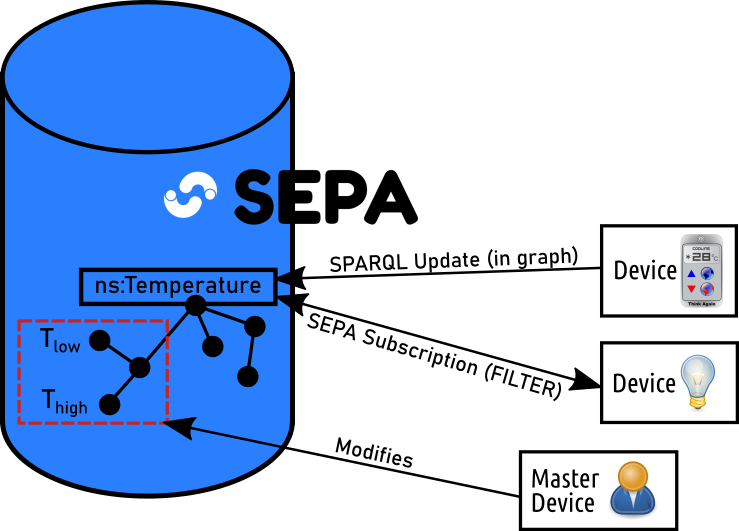
\includegraphics[width=0.7\textwidth]{preferences.png}
\caption{Suggestion for including in Cocktail the concept of \textit{Master Device}, i.e. a device dealing with the user's preferences on context control.}
\label{fig:preferences}
\end{figure*}

A possible alternative, that is currently a preliminary study work still pending implementation is shown in Fig. \ref{fig:preferences} and refers to the Master WebThing concept. First of all, we consider here that the added \texttt{ns:Temperature} resource might be in fact a separate RDF subgraph within SEPA. The temperature graph is required to follow the data schema/field schema concept (see Section \ref{ssec:dataschema_fieldschema}), being formatted in its own specific way. Consequently, any device updating the temperature would make a SPARQL Update similar to the one in Listing \ref{listing:temp_update_subgraph}.

\begin{lstlisting}[caption={SPARQL Update temperature subgraph. Refer to the previous Sections for any unexplained resource. Notice that this is currently (October 2019) an ongoing work and therefore it is not to be considered a final solution.}, label=listing:temp_update_subgraph]
WITH ns:Temperature
DELETE {ns:RoomTemperature swot:hasValue ?v}
INSERT {ns:RoomTemperature swot:hasValue "18.4"}
WHERE {
   ns:RoomTemperature a swot:Data;
   	swot:hasDataSchema ns:MyDoubleDataSchema.
}
\end{lstlisting}

The Master Device on the other hand would take care of the user preferences by modifying the appropriate part of the \texttt{ns:Temperature} subgraph. In our preliminary research we suggest to introduce a new \texttt{swot:Preference} resource type as shown in Listing \ref{listing:pref_update}, defining for the current example the lower and upper boundaries of acceptable temperatures.

Eventually, any device acting due to some temperature specific behaviors would subscribe to that same subgraph, filtering the results according to its own business logic as reported in Listing \ref{listing:pref_subscription}. In this way, each time the temperature falls out of the interval, SEPA triggers the relevant subscriptions based on that resource.

What is still missing in this approach is a complete theory concerning the relationships between different preferences. Are there preferences that are more or less important than others? What would be the effect of this preference ordering in the knowledge base? These are the main future directions for this research.\\
\begin{minipage}{\linewidth}
\begin{lstlisting}[caption={SPARQL Update to temperature preferences. Notice that this is currently (October 2019) an ongoing work and therefore it is not to be considered a final solution.}, label=listing:pref_update]
WITH ns:Temperature
DELETE {
   ns:user_preference ns:lower ?low;
    ns:upper ?high.}
INSERT {
   ns:user_preference ns:lower "18.2";
    ns:upper "28.0".}
WHERE {
   ns:user_preference a swot:Preference.
}
\end{lstlisting}
\end{minipage}
\begin{lstlisting}[caption={Suggested example for SPARQL device FILTER subscription. Notice that this is currently (October 2019) an ongoing work and therefore it is not to be considered a final solution.}, label=listing:pref_subscription]
SELECT ?current
FROM ns:Temperature
WHERE {
   ns:user_preference a swot:Preference;
    ns:lower ?low;
    ns:upper ?high.
   ns:RoomTemperature swot:hasValue ?current.
   FILTER(?current <= ?high)
   FILTER(?current >= ?low)	
}
\end{lstlisting}

Summarizing:
\begin{enumerate}
\item Nothing changes in the PAE interaction paradigm;
\item Target entities like \texttt{ns:Temperature} would be represented as \texttt{swot:Data} within a subgraph;
\item A Master WebThing, described in the same way as other WebThings, would be able to control the user's preferences \texttt{swot:Preference} and modify the target entities accordingly;
\item The devices using the target entities would apply their (autonomous behaviour) business logic based on \texttt{FILTER}ed subscriptions related to \texttt{swot:Preference} instances.
\end{enumerate}

Notice that we have formalized here a \textit{Semantic Belief-Desire-Intention behaviour} \cite{challenger2018development}: the beliefs are the aforementioned subgraphs like \texttt{ns:Temperature}; the desires are the \texttt{swot:Preference} definitions; the intentions are the notification triggers upon \texttt{FILTER}ed subscription.

\subsection{Habitat project example}
The Habitat project acted an essential role in the development of the Semantic Web of Things as intended in this Thesis. Its main contribution, as it will be clear in the next paragraphs, is related to the flexibility in thing description and easy extensibility required to the Habitat IoT-WoT environment. They both had relevant effects in the actual Cocktail implementation.

During the project the author and his colleagues were involved in the creation of an indoor localization IoT environment with the goal of monitoring people with mental impairments. The importance of such systems can be exemplified by a typical use case connected to one of the greatest problems that modern societies are facing, namely the care for people suffering Alzheimer's disease. 

Along with the cognitive decay due to the progression of the disease, it is indeed important to allow the patients to stay safely independent as much as possible so that no stress or technical malfunction could have negative effects on their everyday life. Keeping this in mind, the indoor monitoring provided by Habitat would act as a non invasive control of danger situations, like being close to the stairs, or the patient being almost out of the house without the caregiver supervision.

From a broader point of view indoor monitoring represents a functionality that has various possible applications. Given the versatility of the information retrieved, we have that smartphones apps, social networks, but also police and many others use such information to be more efficient and effective in their jobs of advertising, catching illegal activities and so on.

This is one of the main reasons why the a Semantic approach was preferred within Habitat to control the information flow. The variety of possible usages that can be done of localization information requires a shared and flexible solution for data description. As a consequence, Habitat project outlined on one hand the lower level setup (that are out of the topic of this thesis), i.e. (i) raw data measurements with radio frequency; (ii) fog computing approach retrieving medium-level information, like $(x,y,z)$ coordinates. 

On the other hand, it is important to mention that, on top of the information interoperability, a great achievement was the successful usage of a prototype of Cocktail over SEPA, realizing (iii) information aggregation; (iv) the handling of danger situations by calling the appropriate actuators.

Let us consider point (iv), that was largely addressed in the Sections describing and evaluating Cocktail. Within Habitat we considered two separate possible approaches:
\begin{itemize}
\item If-This-Then-That (IFTTT): the business logic of the IoT environment is realized performing the requests as a set of actions following predetermined conditions. 

\item Rule engines, like Drools \cite{proctor2011drools}: SEPA notifications, in this case, were transformed into events triggering rule evaluation in drools, and resulting eventually in decisions over the environment state.
\end{itemize}

While Habitat project reached its end, there is still the possibility to proceed with some further research in the future. For instance, as the SEPA middleware is common to all these implementations and Cocktail, a good plan would be to study the integration of the two aforementioned techniques within the \texttt{swot:Preference} concept introduced in the previous Section. 

\subsection{Future directions}
This short subsection will list a few possible ideas that could represent some future research directions connected to Cocktail, SEPA, and the applications that were mentioned in the Thesis. 

Indeed, over this Thesis presentation SEPA was largely used and represented an essential tool. The following future directions can be therefore outlined concerning this architecture:
\begin{enumerate}
    \item Study and enhance SEPA's performances. SEPA suffers of quick degradation of performances as the number and complexity of subscriptions grows. Not to mention, the number of triples contained in the knowledge base. This may be a good opportunity to study new algorithms and solutions;
    \item Study the feasibility and the methodology to realize a distributed SEPA, as a single endpoint would clearly not be enough to support the Big Data revolution;
    \item RDF knowledge bases can be exploited with reasoning techniques. Their effect is the modification of the knowledge base according to some rules that could have a huge impact on the whole architecture. Consider, for instance, the situation in which a triple \texttt{?subject-?predicate-?object} is enriched by a reasoner of the \textit{inverse} predicate.
    
A client could remove that inverse triple, because of its own application logic.

The rule effect, however, once aware that the triple is missing, would be to insert it back again and again: how would complex and unexpected behaviors like these interact with the publish-subscribe and with large applications like the SWoT and the IoMusT? The SEPA architecture has not yet been tested with reasoning, and therefore it could be interesting to see how they behave when used together in an application.
\end{enumerate}

Concerning Cocktail and the Semantic Web of Things, there is a need of research that include the implementation of new applications with this framework. A positive feedback of this process, moreover, would be the enhancement of the ontology itself whenever the users come across limits in the definitions or in usage. The framework, also, might be tested as a tool to realize the aforementioned Internet of Musical Things in a WoT flavour, as well as a benchmarking indicator for SEPA performances. Additionally, further research direction related to the semantic knowledge contained in the SWoT would be to extend the semantic context by using for instance DBpedia, and study how this can impact intelligent behaviours within the applications.

\begin{table*}
\centering
\footnotesize
\caption{MIRO Report \cite{matentzoglu2018miro} of the SWOT Ontology -- Part I of III}
\label{tab:miro1}
\begin{tabular}{p{.35\textwidth}p{.65\textwidth}}
\toprule
\multicolumn{2}{c}{\textbf{A. The basics}} \\
\midrule
\textbf{A.1 Ontology name} \textsc{must} & Semantic Web of Things Ontology (SWoT), version 0.1 \\
\textbf{A.2 Ontology owner} \textsc{must}  & Francesco Antoniazzi \\
\textbf{A.3 Ontology license} \textsc{must}  & GNU General Public License v3.0 \\
\textbf{A.4 Ontology URL} \textsc{must} & \url{https://github.com/fr4ncidir/SemanticWoT/blob/master/swot.owl} \\
\textbf{A.5 Ontology repository} \textsc{must}  & \url{https://github.com/fr4ncidir/SemanticWoT} \\
\textbf{A.6 Methodological framework} \textsc{must}  & The ontology is clearly divided into static and dynamic description. The former was developed taking into account previously available works on the Web Thing description made by W3C. An additional part was included, related to data formatting and parametrization. The dynamic part was also studied to be coherent and effective. A proof of concept was given by writing the SPARQL Updates and Queries/Subscriptions needed by the Cocktail framework. \\
\toprule 
\multicolumn{2}{c}{\textbf{B. Motivation}} \\  \midrule
\textbf{B.1 Need} \textsc{must} & The aim of the ontology is to permit the development of Semantic Web of Things applications focusing equally on discovery and accessibility of devices . In fact, as regards this last point, the ontology allows reading properties of Web Things as well as subscribing to their events or invoking their actions. \\
\textbf{B.2 Competition} \textsc{must} & Web of Things ontology~\cite{serena2018discovery} \\
\textbf{B.3 Target audience} \textsc{must} & Developers of Semantic Web of Things applications. \\
\toprule
\multicolumn{2}{c}{\textbf{C. Scope, requirements, development community}} \\  \midrule
\textbf{C.1 Scope and coverage} \textsc{must}  & The ontology defines all the concepts belonging to the Semantic Web of Things domain. The aim of the ontology is to provide a mean for a semantic-enriched interaction with Web Things. This allows developers to exploit semantics for more than just discovering devices. The ontology provides the definitions needed to model the Thing Description as well as the interaction patterns provided by every device.
\\
\textbf{C.2 Development community} \textsc{must} & Advanced Research Center on Electronic Systems (ARCES) of the University of Bologna  \\
\textbf{C.3 Communication} \textsc{must}  & \url{https://github.com/fr4ncidir/SemanticWoT/issues} \\
\midrule
\multicolumn{2}{c}{\textbf{D. Knowledge acquisition}} \\ \midrule
\textbf{D.1 Knowledge acquisition method} \textsc{must}  & Analysis of the literature about Web of Things and experiments carried out at the ARCES department of the University of Bologna in the context of the HABITAT Italian research project and at the Centre for Digital Music (C4DM) of the Queen Mary University of London (QMUL) in the AudioCommons European project. \\
\textbf{D.2 Source knowledge location} \textsc{should}  & -- \\
\textbf{D.3 Content Selection} \textsc{should}  & The main entities to be represented ontology have been selected according to the literature about Web of Things. In fact, the concepts of Web Thing, Property, Event and Action play a crucial role in the ontology. Moreover, to make the ontology suitable to control devices, some classes have been added to map the input and output data. \\
\toprule
\end{tabular}
\end{table*}

\begin{table*}
\centering
\footnotesize
\caption{MIRO Report \cite{matentzoglu2018miro} of the SWOT Ontology -- Part II of III}
\label{tab:miro2}
\begin{tabular}{p{.35\textwidth}p{.65\textwidth}}
\toprule
\multicolumn{2}{c}{\textbf{E. Ontology content}} \\ \midrule
\textbf{E.1 Knowledge representation language} \textsc{must} & OWL 2 generated by  Prot\'eg\'e v5.5.0beta; however, the ontology is at this stage only descriptive, and it uses a reduced subset of OWL 2 capabilities, being the Description Logic ALCRIF(D). \\
\textbf{E.2 Development environment} \textsc{optional} &  Prot\'eg\'e v5.5.0beta \\
\textbf{E.3 Ontology metrics} \textsc{should} & Number of classes: 14; number of object properties: 20; number of data properties: 9; 0 individuals. Application metrics: Web Thing triple count (Equation~\ref{eq:webthing_count}), $DvS$ contents ratio, Data format impact; \\
\textbf{E.4 Incorporation of other ontologies} \textsc{must} & The ontology is stand-alone. Examples are given on how \ontoref{dul, prov, sosa} can be included. See Table~\ref{tab:prefixes}. \\
\textbf{E.5 Entity naming convention} \textsc{must} & Entities follows the CamelCase notation. Both datatype and object properties are named as verb senses with mixedCase notation. \\
\textbf{E.6 Identifier generation policy} \textsc{must} & The SWoT ontology does not Identifiers of the instances must be generated by the application \\
\textbf{E.7 Identity metadata policy} \textsc{must} & All entities have an \texttt{rdfs:comment} natural language explanation. \\
\textbf{E.8 Upper ontology} \textsc{must}& No upper ontology is used in this work, to keep SWoT ontology as close as possible to real applications. A suggestion is given on how to include references to \ontoref{dul} in Fig.~\ref{fig:fig1}.\\
\textbf{E.9 Ontology relationships} \textsc{must}& 20 object properties (plus 20 inverse properties); 9 datatype properties.  \\
\textbf{E.10 Axiom pattern} \textsc{must}& The ontology is not yet to be used with reasoners, but rahter oriented at a clear and operactional definition of the concepts in the Semantic Web of Things. 316 axioms included (of which 175 logical axioms, 7 \texttt{SubClassOf}, 4 \texttt{DisjointClass}, 23 \texttt{SubObjectPropertyOf}, 20 \texttt{InverseProperty}, 5 \texttt{DisjointObjectProperty}, 4 \texttt{FunctionalObjectProperty}, 2 \texttt{IrreflexiveObjectProperty}, 4 \texttt{SubDataPropertyOf}, 8 \texttt{FunctionalDataProperty}, 77 \texttt{AnnotationAssertion}) \\ 
\textbf{E.11 Deferencable URI} \textsc{optional} & Some of the entities of the ontology have been conceived to be reachable from the Web. For instance, thing descriptions, data schemas and field schemas. This is a best practice to be followed, to expand interoperability towards future uses. \\
\toprule
\multicolumn{2}{c}{\textbf{F. Managing change}} \\ \midrule
\textbf{F.1 Sustainability plan} \textsc{must} & The SWoT Ontology will be adopted in wide research projects (as already done with Habitat and AudioCommons). Feedbacks collected during these activities will guide the future development of the ontology. \\
\textbf{F.2 Entity deprecation strategy} \textsc{must}  & No class will be deleted from the ontology. Deprecated classes will be labelled as obsolete with a proper annotation property. \\
\textbf{F.3 Versioning policy} \textsc{must} & The SWOT Ontology adopts sequence-based identifiers for its versions with a major number and a minor number, separated by a dot. A novel release featuring only small changes will cause a switch of the minor number, while relevant and/or structural changes affects also the major number.\\
\toprule
\end{tabular}
\end{table*}

\begin{table*}
\centering
\footnotesize
\caption{MIRO Report \cite{matentzoglu2018miro} of the SWOT Ontology -- Part III of III}
\label{tab:miro3}
\begin{tabular}{p{.35\textwidth}p{.65\textwidth}}
\toprule
\multicolumn{2}{c}{\textbf{G. Quality assurance}} \\ \midrule
\textbf{G.1 Testing} \textsc{must}& The tests for SWoT ontology are closely bound to the ones for the Cocktail framework. A first successful test is the realization itself of all Cocktail's SPARQL enquiries. Secondly, the \texttt{unittest}s available in the repository, allowing to check their consistency by direct usage. \\
\textbf{G.2 Evaluation} \textsc{must}  & Some of the metrics reported in \cite{fernandez2009what} have been used to evaluate the SWOT Ontology. In particular the number of classes, properties and individuals have been measured. Moreover, the maximum and minimum Web Thing triple count, the triple dimension of dynamic interactions and the data format influence on triple dimension have been defined to deal with the dynamic aspect of the ontology.\\
\textbf{G.3 Examples of use} \textsc{must} & An example of the ontology is reported in~\cite{viola2018playsound}. Other examples are available on the GitHub repository: \url{https://github.com/fr4ncidir/SemanticWoT/tree/master/SWTE\_example} \\
\textbf{G.4 Institutional endorsement}  \textsc{optional} & None. \\
\textbf{G.5 Evidence of use} \textsc{must} & Evidences of use are provided by~\cite{viola2018playsound} and~\cite{antoniazzi2017web}. \\
\toprule
& \\
& \\
\multicolumn{2}{c}{\Large SWOT ontology, and Cocktail framework in \faGithub~~~\qrcode{https://fr4ncidir.github.io/SemanticWoT/}} \\
\centering 
\end{tabular}
\end{table*}

%\begin{center}
%\Large \faGithub~~~~\qrcode{https://fr4ncidir.github.io/SemanticWoT/}
%\end{center}
\clearpage

\chapter*{Conclusion}
\addcontentsline{toc}{chapter}{Conclusion}  
\headletter{A}
cross the Chapters of this Thesis a variety of topics were discussed. First of all, we introduced the great Internet of Things revolution, that created in the last twenty years an outstanding opportunity for industry and academy to reach exceptional results. The IoT is now part of everyday life, and its effects on society can only increase in the next years.

A large discussion was then presented reporting the greatest drawback of IoT, i.e., its fragmentation. Also known as ``vertical silos'' fragmentation, this IoT design nightmare is substantially hindering the development of integrated systems due to the difficulty of sharing resource and data among entities that were developed at different time, with different goals, and by different programmers. The various abstraction layers that compose IoT applications need a common way to interact safely and effectively.

The term \textit{interaction}, in this Thesis, is usually intended as \textit{sharing information}. The Semantic Web stack was designed to provide the suitable tools capable of realizing this shared data community. That is, systems would use and design internally their own proprietary data representation, but still agree on a common way to intend resources and relationships on a higher interactive level. Consequently, the Semantic Web could represent a powerful tool to fight IoT fragmentation.

Keeping this idea in mind, we presented some applications related to the Semantic Web: a study on how to visualize it, for diagnostic and didactic purposes; an integration of multiple information sources, within the AudioCommons European project; the SPARQL Event Protocol Architecture, that is the core of the work pursued in the PhD.

The effort of creating a common playground for a fully interoperable IoT through Semantic technologies and protocols led us also to the design and the evaluation of the Internet of Musical Things Ontology. This is a major contribution of the Thesis, as we provide a large description of a shared vocabulary in an innovative and previously mostly unexplored field of the IoT. For the future, we expect to further extend step-by-step the ontology to integrate further IoT application domains in the same description.

Eventually, the Thesis outlines the possibility to realize an implementation of the Web of Things in a semantic fashion. By exploiting the SEPA, in particular, the work here presented shows that the semantic representation of information is capable to keep up with the dynamic evolution of an IoT environment. Consequently, a study is provided on how the Things and their active and passive interactions could be ontologically represented. 

We designed and evaluated, therefore, the Semantic Web of Things Ontology and a framework that realizes the interaction mechanisms over our SEPA architecture. Both the framework and the ontology are an important contribution within the Thesis, and are freely available on Github. This work also led to a publication on the Journal with the highest Impact Factor in the IoT research field (IEEE IoT Journal). Their usage is expected to provide interesting results in future research, for instance by extending the Internet of Musical Things towards the Semantic Web Of Musical Things, as well as enhancing the descriptive capabilities with reasoning mechanisms, or integrating the context with the knowledge of semantic endpoints like DBpedia.

\newpage
\vspace*{\fill}
\begin{center}
\begin{tabular}{p{.3\textwidth}p{.7\textwidth}}
\toprule
\multicolumn{2}{c}{\Large \textbf{Summary of Achievements and Main Contributions I of II}} \\
\midrule
\textbf{IoMusT ontology} & The author of this Thesis realized the ontology engineering work for the IoMusT journal publication (still under revision as for \today). That is, the various sub-components of the ontology were studied to realize the overall integration and functionalities (Section~\ref{ssec:description}). The evaluation part (Section~\ref{ssec:iomust_evaluation}) is also an achievement of the work pursued by the author in this Thesis, given the fact that there is not a standard evaluation mechanism for ontologies. Not to mention, the full \texttt{.owl} file realization through Protégé, and the provided online documentation. \\
& \\
\textbf{SWOT ontology} & The contribution of the author of this Thesis in the SWOT ontology spans over all the steps described in the previous Chapters~\ref{ch:semantic_wot} and \ref{ch:semantic_agent}. In particular, the complete analysis of the work made by the W3C, including the Thing Description conceptualization and the data representation were refactored keeping in mind the SEPA. The ontology, its \texttt{.owl} description, its documentation and the paper published at IEEE IoT Journal \cite{antoniazzi2019building} are the main achievements to be reported here.\\
& \\
\textbf{Cocktail framework} & The author implemented and currently maintains the Cocktail framework presented in the Chapter~\ref{ch:semantic_wot} and available freely on GitHub. Cocktail is a Python3 framework SEPA compatible enabling an easy realization of Semantic WoT environments as described in \cite{antoniazzi2019building}. \\
\bottomrule
\end{tabular}
\end{center}
\vspace*{\fill}
\newpage
\vspace*{\fill}
\begin{center}
\begin{tabular}{p{.3\textwidth}p{.7\textwidth}}
\toprule
\multicolumn{2}{c}{\Large \textbf{Summary of Achievements and Main Contributions II of II}} \\
\midrule
\textbf{Habitat Project} & From mid-2016 until late-2017 the author was involved in the Habitat project: on top of semantic technologies and the SEPA, we realized a radio frequency 2D indoor localization monitoring unit, followed later on by a 3D evolution of the same device. They are both fully integrated in a smart healthcare IoT application environment \cite{borelli2019habitat}. \\
& \\
\textbf{AudioCommons Project} & As explained in the previous Section~\ref{ssec:audiocommons}, the author was involved in the Internet Archive integration within the AudioCommons Mediator. The main achievement, here, was the study performed on the integration among different services addressed with semantic technologies. \\
& \\
\textbf{Visualization of \mbox{Semantic} Knowledge Bases} & Working with ontologies both at teaching level and at a research level outlined over the time in ARCES research group the need for tools that would help us in explaining the contents of ontologies and Knowledge Bases. The achievements reached in this field by the author are in one hand a survey over the tools already available \cite{antoniazzi2018rdf} and, in the other hand, the collaboration in the realization of another tool specific for teaching purposes, named Tarsier \cite{viola2018interactive}. This work was helpful to study and prepare the SWOT ontology and the IoMusT ontology.\\
\bottomrule
\end{tabular}
\end{center}
\vspace*{\fill}


\makeatletter
\chapter*{List of Ontologies \& Prefixes}
\label{sec:ontology_list}
\addcontentsline{toc}{chapter}{List of Ontologies \& Prefixes}
\small
\begin{enumerate}
\itemsep15pt
\renewcommand{\labelenumi}{\textbf{\theenumi}}
\item[\texttt{foaf}~-~] The \textit{Friend of a friend} ontology is a basic ontology used to describe links between people. \\
Developed by \hfill FOAF project, RDF and Semantic Web community \\
Available at \hfill \url{http://xmlns.com/foaf/spec/} \\
SPARQL prefix \hfill \texttt{http://xmlns.com/foaf/0.1/} \\
Reference \hfill \url{http://www.foaf-project.org/}

\item[\texttt{prov}~-~] The \textit{Provenance of Information} ontology is a basic ontology used to describe how agents exchange information . \\
Developed by \hfill W3C \\
Available at \hfill \url{https://www.w3.org/TR/prov-o/} \\
SPARQL prefix \hfill \texttt{http://www.w3.org/ns/prov\#}

\item[\texttt{ssn}, \texttt{sosa}~-~] The \textit{Semantic Sensor Network} ontology, and its core \textit{Sensor, Observation, Sample, and Actuator} ontology, are the basic approach to represent semantically sensors and actuators in their environment. \\
Developed by \hfill W3C \\
Available at \hfill \url{https://www.w3.org/TR/vocab-ssn/} \\
SPARQL prefixes \hfill \texttt{http://www.w3.org/ns/ssn/} \\
\null \hfill \texttt{http://www.w3.org/ns/sosa/}

\item[\texttt{event}~-~] The \textit{Event} ontology deals with sequences of events, providing the tools to identify actors and relationships among them. \\
Developed by \hfill Centre for Digital Music, Queen Mary University of London \\
Available at \hfill \url{http://motools.sourceforge.net/event/event.html} \\
SPARQL prefix \hfill \texttt{
http://purl.org/NET/c4dm/event.owl\#}

\item[\texttt{timeline}~-~] The \textit{Timeline} ontology is an ontology used to annotate any kind of time-related resource. \\
Developed by \hfill Centre for Digital Music, Queen Mary University of London \\
Available at \hfill \url{http://motools.sourceforge.net/timeline/timeline.html} \\
SPARQL prefix \hfill \texttt{http://purl.org/NET/c4dm/timeline.owl\#}

\item[\texttt{mo}, \texttt{music}~-~] The \textit{Music} ontology is a modelization that provides a common vocabulary to address all kind of music-related information. \\
Developed by \hfill     Yves Raimond, Thomas Gängler, Frédérick Giasson,\\
\null \hfill Kurt Jacobson, George Fazekas, Simon Reinhardt, Alexandre Passant \\
Available at \hfill \url{http://musicontology.com/}\\
SPARQL prefix \hfill \texttt{http://purl.org/ontology/mo/}\\
Reference \hfill \cite{raimond2007music, raimond2010spec}

\item[\texttt{studio}~-~] The \textit{Studio} ontology, compared to the Music ontology, models the music production activity in a recording studio environment. \\
Developed by \hfill Centre for Digital Music, Queen Mary University of London \\
Available at \hfill  \url{http://isophonics.net/content/studio-ontology}\\
SPARQL prefix \hfill \textit{not available}\\
Reference \hfill \cite{fazekas2011studio}

\item[\texttt{afo}~-~] The \textit{Audio Features} ontology describes the features of audio signals, and exploits the Event and the Timeline ontologies. \\
Developed by \hfill Centre for Digital Music, Queen Mary University of London \\
Available at \hfill  \url{http://motools.sourceforge.net/doc/audio_features.html}\\
SPARQL prefix \hfill \textit{not available}\\
Reference \hfill \cite{allik2016ontology}

\item[\texttt{dul}~-~] The \textit{DOLCE+DnS Ultralite} (DUL) ontology, with reference to the website, aims to provide a collection of upper-level concepts, to foster alignment among ontologies and semantic setups. \\
Developed by \hfill Aldo Gangemi, Nicola Guarino, Claudio Masolo\\
\null \hfill Alessandro Oltramari, Luc Schneider \\
Available at \faLevelDown \hfill \null \\
\null \hfill \url{http://ontologydesignpatterns.org/wiki/Ontology:DOLCE\%2BDnS_Ultralite} \\
SPARQL prefix \hfill \texttt{http://www.ontologydesignpatterns.org/ont/dul/DUL.owl} \\
Reference \hfill \cite{gangemi2002sweetening}

\item[\texttt{swot}~-~] The \textit{Semantic Web of Things} ontology is a work that organizes a new vision of the Web of Things, compatible with semantic technologies, to overcome the fragmentation of IoT. \\
Developed by \hfill Francesco Antoniazzi, Fabio Viola \\
Available at \hfill \url{https://w3id.org/swot\#}\\
SPARQL prefix \hfill \null \texttt{http://www.semanticweb.org/unibo/antoniazzi/2019/0/swot} \\
Reference \hfill \cite{antoniazzi2019building}

\item[\texttt{iot}, \texttt{iomust}~-~] The \textit{Internet of Musical Things} ontology aims to provide the instruments to define an IoT environment for music. It is fully described in Section~\ref{sec:iomust}. \\
Developed by \hfill Francesco Antoniazzi \\
Available at \hfill \url{https://w3id.org/iomust\#}\\
SPARQL prefix\faLevelDown \hfill \null \\
\null \hfill \texttt{http://www.semanticweb.org/iot/ontologies/2019/5/internet\_of\_things} \\
Reference \hfill \textit{under review}

\item[\texttt{collection}~-~] The \textit{Collection} ontology is used to define a common vocabulary to represent collections, lists, bags of items, and their relationships.\\
Developed by \hfill Paolo Ciccarese, Silvio Peroni \\
Available at \hfill \url{https://code.google.com/archive/p/collections-ontology/}\\
SPARQL prefix \hfill \texttt{http://purl.org/co\#}\\
Reference \hfill \cite{ciccarese2014collections}

\item[\texttt{dc}~-~] The \textit{Dublin Core} ontology was defined to describe metadata. It contains, for instance, the authorship relation, and is commonly used to describe even meta information on ontologies. \\
Developed by \hfill The Dublin Core Metadata Initiative (DCMI) \\
Available at \hfill \url{https://www.dublincore.org/specifications/dublin-core/} \\
SPARQL prefix \hfill \texttt{http://purl.org/dc/elements/1.1/} \\
\null \hfill \texttt{http://purl.org/dc/terms/} \\
Reference \hfill \cite{weibel2000dublin}, \\
\null \hfill \url{https://www.dublincore.org/specifications/dublin-core/dcmi-terms/2012-06-14/?v=terms}

\item[\texttt{aco}~-~] The \textit{Audio Commons} Ontology provides main concepts and properties for describing audio content, both musical and non-musical, on the Semantic Web. \\
Developed by \hfill George Fazekas, Miguel Ceriani \\
Available at \hfill \url{http://www.audiocommons.org/ac-ontology/aco.html} \\
SPARQL prefix \hfill \texttt{https://w3id.org/ac-ontology/aco\#} \\
Reference \hfill \cite{ceriani2018audio} \\
\end{enumerate}

\vspace*{1.5cm}
\begin{table}[!h]
\centering \footnotesize
\caption{Expanded SPARQL prefixes}
\label{tab:prefixes}
\begin{tabular}{ll}
\textbf{Prefix}    &   \textbf{URI}    \\ \hline
\texttt{rdf:}    &   \texttt{http://www.w3.org/1999/02/22-rdf-syntax-ns\#} \\ \hline
\texttt{rdfs:}   &   \texttt{http://www.w3.org/2000/01/rdf-schema\#}\\ \hline
\texttt{owl:}    &   \texttt{http://www.w3.org/2002/07/owl\#} \\ \hline
\texttt{iot:}   &   \texttt{http://www.semanticweb.org/iot/ontologies/2019/5/internet\_of\_things/}\\ \hline  
\texttt{iomust:}    &  \texttt{http://www.semanticweb.org/iot/ontologies/2019/5/internet\_of\_things/iomust/} \\ \hline
\texttt{mo, music:}    &   \texttt{http://purl.org/ontology/mo/}\\ \hline
\texttt{prov:}   &   \texttt{http://www.w3.org/ns/prov\#} \\ \hline
\texttt{sosa:}   &  \texttt{http://www.w3.org/ns/sosa/} \\ \hline
\texttt{co:}   &  \texttt{http://purl.org/co\#} \\ \hline
\texttt{foaf:}   &  \texttt{http://xmlns.com/foaf/0.1/} \\ \hline
\texttt{event:}   &  \texttt{http://purl.org/NET/c4dm/event.owl\#} \\ \hline
\texttt{timeline:}   &  \texttt{http://purl.org/NET/c4dm/timeline.owl\#} \\ \hline
\texttt{dbpedia:} &  \texttt{http://dbpedia.org/resource/} \\ \hline
\texttt{dbpo:} & \texttt{http://dbpedia.org/ontology/} \\ \hline
\texttt{ns:} &  \textit{whatever personal valid namespace} \\ \hline
\end{tabular}
\end{table}

\addcontentsline{toc}{chapter}{List of Figures}
\listoffigures
\addcontentsline{toc}{chapter}{List of Tables}
\listoftables
\newpage

\addcontentsline{toc}{chapter}{Bibliography}
\bibliographystyle{IEEEtran}
\begin{multicols}{2}
\footnotesize
\bibliography{biblio}
\end{multicols}

%\chapter*{Thanks}
%\addcontentsline{toc}{chapter}{Thanks} 
%\input{thankyou.tex}

%\input{Relazione.tex}

\end{document}  